\documentclass
[a4paper,14pt,russian]{article}
\usepackage{extsizes}
\usepackage{cmap}     
\usepackage{mathtext}                       % для кодировки шрифтов в pdf
\usepackage{multirow}
\usepackage[T1, T2A, TS1]{fontenc}
\usepackage{paratype}
\usepackage[utf8]{inputenc}                  % для кодировки текста в UTF8
\usepackage[russian]{babel}
%\usepackage{pscyr}
\usepackage{textcomp}                            % красивые шрифты для кириллицы
\usepackage{url}
%\usepackage[linktoc=all]{hyperref}
\urlstyle{rm} 
%\renewcommand{\rmdefault}{ftm}               % Times New Roman
\usepackage{alltt} % вставка исходынх кодов
% --- отступы по ГОСТу
\usepackage{geometry}
\geometry{left=2.1cm}
\geometry{right=1cm}
\geometry{top=2cm}
\geometry{bottom=2cm}

\usepackage{graphicx}                        % для вставки изображения
\graphicspath{{pics/}}                       % директория с изображениями (иначе не будет проставлять номера в ссылках)

\usepackage{amssymb,amsfonts,amsmath,amsthm} % математические дополнения от АМС
\usepackage{indentfirst}                     % отделять первую строку раздела абзацным отступом тоже
\usepackage[usenames,dvipsnames]{color}      % названия цветов 
\usepackage{ulem}                            % подчеркивания
\usepackage{array}
%для списка литературы
\usepackage{etoolbox}

% --- полуторный интервал между строками
\usepackage{setspace}
\onehalfspacing

\setcounter{tocdepth}{3}                     % глубина просмотра уровней разделов для формирования оглавления
\setcounter{secnumdepth}{3}                  % глубина просмотра уровней разделов для их нумерации в оглавлении

\parindent=15mm                              % абзацный отступ
\renewcommand{\labelitemi}{--}               % задание маркера для первого уровня ненумерованных списков (тире)
\renewcommand*\labelenumi{\theenumi.}        % задание вида первого уровня нумерованных списков (цифра со скобкой)
\renewcommand{\labelenumii}{\arabic{enumi}.\arabic{enumii}.}

\setcounter{secnumdepth}{5}	%нумерация  subsubsub - параграфа
%\renewcommand\contentsname{Оглавление}


\makeatletter
\renewcommand{\@biblabel}[1]{#1.} % Заменяем библиографию с квадратных скобок на точку:
\patchcmd{\thebibliography}{\section*{\refname}}{}{}{}

% делаем перенос после параграфа
\renewcommand\paragraph{%
   \@startsection{paragraph}{4}{0mm}%
      {-\baselineskip}%
      {.5\baselineskip}%
      {\normalfont\normalsize\bfseries}}
  
% убираем вылеты за поля 
\sloppy
\righthyphenmin=2

\usepackage{float}

%изменение подписей к рисункам на "Рисунок 1 - название" и "Таблица 1 - название
\usepackage[singlelinecheck=false]{caption}
\DeclareCaptionLabelSeparator{defffis}{ -- }
\captionsetup[figure]{justification=centering,labelsep=defffis}
\captionsetup[table]{justification=raggedright, labelsep=defffis}
\addto\captionsrussian{\def\figurename{Рисунок}}

% делаем горизонтальную ориентацию
\usepackage{afterpage}
\usepackage{pdflscape}

%убиираем висячие строки
\clubpenalty=10000
\widowpenalty=10000


\renewcommand\appendixname{Приложение}
\makeatletter
\def\redeflsection{\def\l@section{\@dottedtocline{1}{1.5em}{7.8em}}}
\renewcommand\appendix{\par
\setcounter{section}{0}%
\setcounter{subsection}{0}%
\def\@chapapp{\appendixname}%
\addtocontents{toc}{\protect\redeflsection}
%\def\thesection{\appendixname\hspace{0.2cm}\@arabic\c@section}}
\def\thesection{\appendixname\hspace{0.2cm}\@Alph\c@section}}
\makeatother

%-----------------------------------------------------------------------------------------------------------------------



\begin{document}
\newpage 
~
\newpage
~
\renewcommand{\arraystretch}{1.4} %% increase table rowspacing   
\newpage
\section*{Реферат}
Данная расчетно-пояснительная записка содержит 165 страниц, 47 иллюстраций, 29 таблиц, 2 приложения, 20 использованных источников.


 
\newpage
                          		                         
\tableofcontents                         

\newpage
\section*{Нормативные ссылки}
\addcontentsline{toc}{section}{Нормативные ссылки}
В дипломном проекте использованы следующие стандарты:

ГОСТ 19.001-77. <<Единая система программной документации. Общие положения>>;

ГОСТ 19.105-78. <<Единая система программной документации. Общие требования к программным документам>>;

ГОСТ 19.106-78. <<Единая система программной документации. Требования к программным документам, выполненным печатным способом>>;

ГОСТ 34.602-89 <<Техническое задание на создание автоматизированной системы>>

ГОСТ 9327. <<Бумага и изделия из бумаги. Потребительские форматы>>;

ГОСТ 1.5. <<Государственная система стандартизации РФ. Общие требования к построению, изложению, оформлению и содержанию стандартов>>;

ГОСТ 2.105. <<Единая система конструкторской документации. Общие требования к текстовым документам>>;

ГОСТ 6.38. <<Унифицированные системы документации. Система организационно-распорядительной документации. Требования к оформлению документов>>;

ГОСТ 7.1. <<Система стандартов по информации, библиотечному и издательскому делу. Сведения об источниках>>;

ГОСТ 7.12. <<Система стандартов по информации, библиотечному и издательскому делу. Реферат и аннотация. Общие требования>>;

ГОСТ 7.32-2001. <<Система стандартов по информации, библиотечному и издательскому делу. Отчет о научно-исследовательской работе. Структура и правила оформления>>;

СанПиН 2.2.2/2.4.1340-03 <<Гигиенические требования к персональным электронно-вычислительным машинам и организации работы>>.

\newpage
\section*{Определения, обозначения и сокращения}
\addcontentsline{toc}{section}{Определения, обозначения и сокращения}

В расчетно-пояснительной записке использованы следующие Определения, обозначения и сокращения:

API - интерфейс программирования приложений. набор готовых классов, процедур, функций, структур и констант, предоставляемых приложением (библиотекой, сервисом) для использования во внешних программных продуктах.

Android -  операционная система для смартфонов, планшетных компьютеров, электронных книг, цифровых проигрывателей, наручных часов, игровых приставок, нетбуков, смартбуков, очков Google и других устройств. Основана на ядре Linux и собственной реализации Java от Google.

C++ - компилируемый статически типизированный язык программирования общего назначения.

GPS - Global Positioning System.  Спутниковая система навигации, обеспечивающая измерение расстояния, времени и определяющая местоположение во всемирной системе координат. 

Java -  объектно-ориентированный язык программирования, разработанный компанией Sun Microsystems.

MATLAB -  пакет прикладных программ для решения задач технических вычислений и одноимённый язык программирования, используемый в этом пакете.

SDK - комплект средств разработки, который позволяет специалистам по программному обеспечению создавать приложения для определенного пакета программ, программного обеспечения базовых средств разработки, аппаратной платформы, компьютерной системы, игровых консолей, операционных систем и прочих платформ.

SLAM - Simultaneous Location and Mapping. Метод, используемый роботами и автономными транспортными средствами для построения карты в неизвестном пространстве или для обновления карты в заранее известном пространстве с одновременным контролем текущего местоположения и пройденного пути.

ИИУ - инерционное измерительное устройство. Устройство включающее в себя датчики линейного ускорения (акселерометры) и угловой скорости (гироскопы или пары акселерометров, измеряющих центробежное ускорение).  
 
СЛАУ - система линейных алгебраических уравнений.
Дрейф нуля - самопроизвольное изменение выходного сигнала со временем при неизменном или даже отсутствующем входном сигнале.

ГЛОНАСС - глобальная навигационная спутниковая система. советская и российская спутниковая система навигации, разработана по заказу Министерства обороны СССР.

Одомтерия - использование данных о движении приводов, для оценки перемещения. Так же термин применяется для любого метода оценки перемещения.

ПЗС - прибор с зарядовой связью, специализированная аналоговая интегральная микросхема, состоящая из светочувствительных фотодиодов, выполненная на основе кремния.

Фреймворк - структура программной системы; программное обеспечение, облегчающее разработку и объединение разных компонентов большого программного проекта. 

\newpage

\section{Конструкторская часть}

\subsection{Разработка технического задания}
\subsubsection{Постановка задачи проектирования}

Целью разработки подсистемы автономного определения перемещения объекта является предоставления удобного с точки зрения интеграции компонента для встраивания во многие бытовые автономные автоматические системы,  в то же время дешевого и не требующего специализированных устройств для своей работы.

\subsubsection{Описание предметной области}
\paragraph{Естественно-языковое описание процесса.}

В ходе создания подвижных автономных систем возникает задача определения текущего местоположения объекта в пространстве.

Для этого можно использовать различные методы, основанные на глобальном позиционировании в географической системе координат с использованием позиционирования по спутникам (GPS, ГЛОНАСС), или методы, основанные на определении перемещения от стартовой позиции. При этом у данных методов разные сферы применения. Так, например, при позиционировании внутри помещения использование спутниковых систем позиционирвоания становиться невозможным по причине слабого сигнала или его полного отсутсвтвия, а так же из-за недостаточной точности в рамках навигации внутри интерьера помещения. Так же не стоит забывать про акутальность систем навигации в космической отрасли, где использование спутников является невозможным впринципе. 
Вторую группу методов принято называть методами одометрии, которые могут быть основаны на:
\begin{itemize}
\item на вращении колес;
\item использовании инерциальных измерительных приборов;
\item компьютерном зрении.
\end{itemize}

Каждый из них обладает своими плюсами и минусами \cite{odometryMethods}, но развитие вычислительной техники и алгоритмов компьютерного зрения дало мощный толчок к более широкому применению визуальной одометрии. Данный подход позволяет получать один видеоряд через видеокамеру и на его основе получать разные сведения об окружающей среде. Тем не менее он не лишен недостатков. Для борьбы с ними применяется комбинация нескольких методов одомтерии. 

Одним из вариантов сомещения методов является использование метода визуальной одометрии и инерционных измерительных устройств. 

При таком гибридном методе данные с видеокамеры и данные с инерционных измерительных устройств обрабатываются параллельно и независимо. В результате получаются два независимых рассчитынных положения носителя, после чего они сопоставляются, и из них выбираются наиболее правдоподобные. 

Таким образом, в процессе функционирования спроектированного модуля визуальной одометрии происходит следующий бесконечный процесс. 
На вход модуля непрерывно подается видео поток и данные об угловых скоростях и ускорении объекта относительно трех взаимноперпендикулярных осей. Эти данные обрабатываются параллельно в соответствующих модулях, на выходе каждого из которых получаем смещение объекта относительно предыдущего положения и его поворот. Далее эти данные совмещаются и выбираются наиболее правдоподобные, которые затем прибавляются к положению и углу поворота, высчитанным на предыдущей итерации. 


\paragraph{Графическое представление процесса}
Графическое представление процесса процесса представлено на рисунке~\ref{pic:predmetOblast}.

\begin{figure}[!htb]
\center{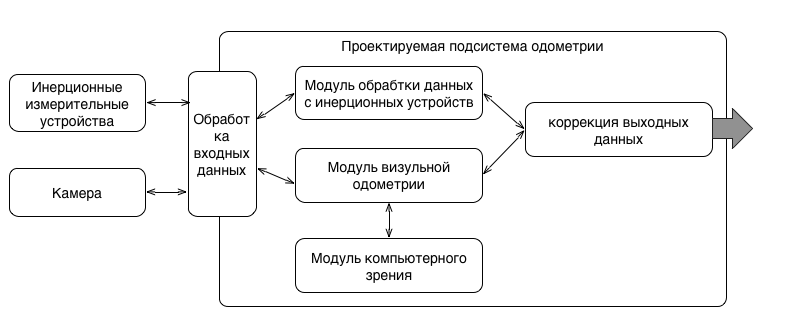
\includegraphics[width=0.8\linewidth]{pics/predmetOblast.png}}
\caption{Графическое представление процесса.}
\label{pic:predmetOblast}
\end{figure}

\paragraph{Вычисление оптического потока.}

\textbf{Оптический поток} — это изображение видимого движения объектов, поверхностей или краев сцены, получаемое в результате перемещения наблюдателя (глаз или камеры) относительно сцены\cite{wikiOpticalFlow}.

Существует несколько подходов к определению смещений между двумя соседними кадрами. Например, можно для каждого небольшого фрагмента (скажем, 8 на 8 пикселей) одного кадра найти наиболее похожий фрагмент на следующем кадре. В этом случае разность координат исходного и найденного фрагментов даст нам смещение. Основная сложность тут состоит в том, как быстро отыскать нужный фрагмент, не перебирая весь кадр пиксель за пикселем. Различные реализации этого подхода так или иначе решают проблему вычислительной сложности. Некоторые настолько успешно, что применяются, например, в распространенных стандартах сжатия видео. Платой за скорость естественно является качество. Мы же рассмотрим другой подход, который позволяет получить смещения не для фрагментов, а для каждого отдельного пикселя, и применяется тогда, когда скорость не столь критична. Именно с ним в литературе часто связывают термин “оптический поток”.

Данный подход часто называют дифференциальным, поскольку в его основе лежит вычисление частных производных по горизонтальному и вертикальному направлениям изображения. Как мы увидим далее, одних только производных недостаточно чтобы определить смещения. Именно поэтому на базе одной простой идеи появилось великое множество методов, каждый из которых использует какую-нибудь свою математическую пляску с бубном, чтобы достичь цели. Сконцентрируемся на методе Лукаса-Канаде (Lucas-Kanade), предложенном в 81 году Брюсом Лукасом и Такео Канаде. Данный метод является наименее ресурсоемким  \cite{habrOpticalFlowAbout} при этом обеспечивает приемлемое качество вычисления оптического потока. 

С математической точки зрения данный алгоритм можно описать следующим образом.
Пусть даны два изображения $F1$ и $F2$, и нам требуется найти смещение точки с координотой $x$. Рассматривая два последовательных изображения можно сказать:
$$ f_2(x) = f_1 (x-d)$$
Обратите внимание, что $f_1$ и $f_2$ при желании можно записать и в общем виде: $f_1(x) = I (x, y, t)$ ; $f_2(x) = I (x, y, t+1)$.

Свяжем известные значения со смещением d. Для этого запишем разложение в ряд Тейлора для $ f_1 (x-d)$:
$$  f_1 (x-d) =f_1(x) + df_1'(x) + O(d^2f_1'') $$
Предположим, что $ f_1 (x-d)$ достаточно хорошо аппроксимируется первой производной. Сделав это предположение, отбросим всё что после первой производной:
$$  f_1 (x-d) =f_1(x) + df_1'(x) $$

Смещение $d$ — это наша искомая величина, поэтому необходимо преобразовать $ f_1 (x-d)$ . Как мы условились ранее, $ f_2(x) = f_1 (x-d) $, поэтому просто перепишем:
$$ f_2(x)= f_1(x) - df_1'(x) $$
Отсюда следует:
$$ d = \frac{f_1(x)-f_2(x)}{f_1'(x)} $$

Следует отметить, что выше был рассмотрен одномерный случай и были сделаны несколько грубых допущений. Но описание алгоритма Лукаса-Канаде для двумерного случая только усложняет математические выводы и понимание сути. 

Для снижения погрешности вызванной отбрасыванием старших производных смещение для каждой пары кадров (назовём их $F_i$ и $F_{i+1}$) можно вычислять итеративно. В литературе это называется искажением (warping). На практике это означает, что, вычислив смещения на первой итерации, мы перемещаем каждый пиксель кадра $F_{i+1}$ в противоположную сторону так, чтобы это смещение компенсировать. На следующей итерации вместо исходного кадра $F_{i+1}$ мы будем использовать его искаженный вариант $F_{i+1}^1$. И так далее, пока на очередной итерации все полученные смещения не окажутся меньше заданного порогового значения. Итоговое смещение для каждого конкретного пикселя мы получаем как сумму его смещений на всех итерациях \cite{habrOpticalFlowTheory}.

Так же следует отметить, что данный алгоритм плохо работает на однотонных изображениях. Данный недостаток является самым критичным. 

\paragraph{Одометрия с использованием инерциальных измерительных устройств}
Навигационные решения надлежащего качества могут быть получены именно в результате взаимодействия или последующей совместной обработки данных от двух  источников - визуальной одометрии и инерциальной системы.  

В наиболее общей форме можно определить инерциальную систему как ортогональную триаду гироскопов и акселерометров, выполняющих непосредственные геопространственные измерения и вычислительный блок, осуществляющий алгоритмические преобразования данных непосредственных измерений.

Следует отметить, что гироскоп любого типа позволяет определять ориентацию в геодезическом пространстве в любой момент времени независимости от местоположения, скорости и других параметров носителя. Точность поставляемых гироскопом данных во всех случаях подвержена деградации («ухода») с течением времени. Величина «ухода» значительна и может составлять до нескольких градусов в час \cite{laserLocation}.

Акселерометры предназначены для измерения линейных ускорений. В равной степени они пригодны для измерений сил, так как согласно ньютоновской механике сила и ускорение есть разные проявления одного и того же физического явления.

В общем случае в системах навигации следует определять следующие показатели:
\begin{itemize}
\item \textbf{Рыскание} — угловые движения летательного аппарата, судна, автомобиля относительно вертикальной оси (см. также вертикальная ось самолёта), а также небольшие изменения курса вправо или влево, свойственные судну \cite{wikiRiskanie};
\item \textbf{Крен} — поворот объекта (судна, самолёта, фундамента) вокруг его продольной оси \cite{wikiKren};
\item \textbf{Тангаж} — угловое движение летательного аппарата или судна относительно главной (горизонтальной) поперечной оси инерции \cite{wikiTangazh}.

\end{itemize}
С учетом сделанных замечаний рассмотрим основные процедуры, выполняемые в навигационном комплексе на базисном уровне.

\textit{\textbf{Вычисление крена и тангажа посредством акселерометров}}

Обладая чувствительностью к земной гравитации, акселерометры обеспечивают измерение долговременных значений крена и тангажа по схеме, изображенной на рисунке~\ref{pic:tangazh}. Рассмотрим акселерометр, рабочая ось которого совпадает со строительной осью $oX$ носителя.

\begin{figure}[!htb]
\center{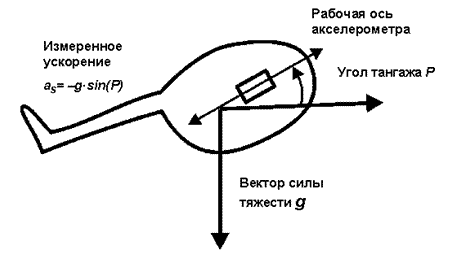
\includegraphics[width=0.6\linewidth]{pics/tangazh.png}}
\caption{Измерения величин крена и тангажа посредством акселерометров.}
\label{pic:tangazh}
\end{figure}

Полагая ускорение носителя равным нулю, мы можем вычислить угол тангажа как:
$$P = \arcsin (-a_s/g)$$

Аналогично вычисляется угол крена. Таким образом, два из трех углов, определяющих угловую ориентацию, могут быть определены только за счет использования акселерометров. Это совершенно очевидный результат, принимая во внимание то обстоятельство, что углы крена и тангажа по изначально определены по отношению к вертикали, которая в нашем случае соответствует вектору тяжести. Однако, здесь следует признать, что описанный метод не может быть использован на практике сам по себе, так как в описанной схеме существенно состояние покоя, в котором должна находиться система. Если это условие не соблюдается, то совершенно очевидно, что отсутствует принципиальная возможность выделить вектор ускорения свободного падения из суммы всех ускорений, которую испытывает система.

\textit{\textbf{Вычисление изменений ориентации с использованием гироскопов}}

Как отмечено выше, в конструкции навигационного комплекса используются оптические гироскопы, обладающие чувствительностью к изменениям ориентации т.е. к величине угловой скорости. Интегрирование (численное суммирование) значений, измеренных гироскопами, обеспечивает определение кратковременных угловых перемещений в физическом пространстве.

Для корректного расчета угла поворота должны быть учтены
внутренние ошибки гироскопа – дрейф, ошибка масштабного коэффициента, случайный шум.

При этом внутренние ошибки  гироскопа полностью смешаны с истинными значениями и не могут быть отделены от них на базисном информационном уровне. В процессе дальнейшей обработки эта смесь подвергается интегрированию, в результате чего возникает ошибочное угловое смещение, которое, таким образом, приобретает долговременный характер (рис. ~\ref{pic:acell}). Точная оценка величины ошибочного углового смещения и его устранение осуществляется при генерации навигационного решения на последующем навигационном уровне.

\begin{figure}[!htb]
\center{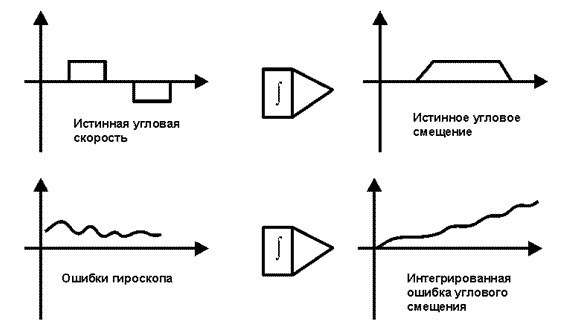
\includegraphics[width=0.6\linewidth]{pics/acelerometr.png}}
\caption{Схема определения углового смещения.}
\label{pic:acell}
\end{figure}

\textit{\textbf{Определение координат пространственного положения с помощью акселерометров.}}

Наличие акселерометров позволяет определять величины линейных ускорений, которые испытывает система. Положим, что ориентация системы в физическом пространстве определена точно с помощью методов, описанных выше. Тогда имеется возможность выделить вектор силы гравитации среди всей суммы векторов сил, приложенных к системе и, следовательно, оценить величину ускорения. Численное интегрирование ускорения позволяет перейти к скорости, а повторное интегрирование к перемещению. Таким образом, с учетом представленных выше замечаний и правилах перехода из физического пространства в географическое, появляется принципиальная возможность оценить геодезические координаты системы в любой момент времени.

\paragraph{Корректировка выходных данных}

\paragraph{Анализ функций, подлежащих автоматизации}

\subsubsection{Выбор критериев качества}
Выделим основные критерии, по которым следует оценивать разрабатываемую подсистему.
\begin{itemize}
\item \textbf{Необходимость в специальном оборудовании} - исходя из задачи, предполагается использование проектируемого модуля в низкобюджетных системах. В связи с этим необходимо обеспечить корректную работу подсистемы с неспециальным оборудованием таким, как бытовые камеры. 
\item \textbf{Стоимость необходимого оборудования} – исходя из предыдущего пункта, следует обеспечивать поддержку наиболее дешевого оборудования. 
\item \textbf{Сложность интеграции} – в современном мире наличия многих конкурентов и налогов одним из ключевых факторов при выборе между ними является простота использования продукта. В связи с этим необходимо снизить время, необходимое на интеграцию с разрабатываемой подсистемой, путем предоставления удобного в использовании API.
\item \textbf{Точность} - данный критерия является важным для задач определения положения в пространстве априори, так как при низкой точности использование систем данного рода становится бесмысленным. Тем не менее в рамках многих задач обеспечение чрезмерно высокой точности является избыточным.
\item \textbf{Возможность свободного использования} – нередко разработчики программных или аппаратных продуктов накладыают ограничение в виде разного рода лицензий распространения, которые ограничивают пользователей в распространении и использовании своих продуктов. В связи с этим важным явлется свободность использования продукта в любых целях, не  противоречящих законодательству стран, где проихсходит его использование.
\end{itemize}

\subsubsection{Анализ аналогов и прототипов}


\paragraph{Сравнительный анализ}

Для сравнения представленных вариантов воспользуемся методом взвешенной суммы. Данный метод позволяет объединить ряд критериев сравнения в один интегральный показатель, по которому затем выбирается наилучший вариант, соответствующий максимальному значению этого интегрального показателя. Метод взвешенной суммы можно представить следующим образом: 
$$ Y = \max_{j \ni m} \displaystyle\sum_{i=1}^{n} \alpha_i \cdot K_{ij},$$
где $\sum_{i=1}^{n} \alpha_i = 1$

По этому критерию проводится сравнение $j (j = 1, 2, …, m)$ вариантов по $i (i = 1, 2, …, n)$ показателям, где:

$n$ – количество показателей сравнения;

$m$ – количество вариантов сравнения.

$K_{ij}$ – нормированный коэффициент соответствия $i$-ого параметра $j$-ого варианта эталонному значению, т.е. для $j$-ого варианта:
$$ K_{ij} = \frac{\max_{j} X_{ij}} {X_{ij}}, $$
$$ 0 < K_{ij} < 1 $$
Соответствие систем-аналогов выбранным критериям качества представлено в Таблице

\subsubsection{Перечень задач, подлежащих решению в процессе разработки}

Исходя из приведенного выше первичного анализа предметной области можно сформировать список задач, подлежащих решению.

Необходимо решить следующие задачи:

\begin{enumerate}
\item разработка структуры и архитектуры подсистемы системы; 
\item разработка требований к формату и структуре передаваемых данных;
\item разработка алгоритмов обработки информации;
\item выбор и обоснование КТС, необходимого для реализации системы;
\item разработка графа диалога и набора экранных форм;
\item оценка предполагаемого качества функционирования системы;
\item организационно-экономическое обоснование разработки;
\item рекомендации по охране труда.
\end{enumerate}





\subsection{Проектирование подсистемы}
\subsubsection{Разработка структуры подсистемы}
\paragraph{Определение состава компонентов}

Исходя из анализа функций структурно в подсистеме можно выделить следующие основные части:
\begin{itemize}
\item \textbf{модуль обработки входных данных} (преобразует входные данные в удобоваримый вариант для последующей обработки);
\item \textbf{модуль компьютерного зрения }(позволяет обрабатывать изображения и производить их анализ для построения визуальной одометрии);
\item \textbf{модуль визуальной одометрии} (высчитывает перемещение и угол поворота камеры на основе последовательности изображений);
\item \textbf{модуль обработки данных с инерционных приборов} (производит математическую обработку показаний датчиков и на ее основе вычисляет перемещение объекта);
\item \textbf{модуль сопоставления  и вывода данных} (сравнивает показания двух предыдущих модулей и на их основе выводит наиболее правдоподобное положение объекта).
\end{itemize}

\paragraph{Определение структуры компонентов}
Согласно общепринятой терминалогии система состоит из подсистем, а те в свою очередь из модулей. Таким образом разрабатываемая подсистема состоит из следующих модулей:

\begin{itemize}
\item обработки входных данных;
\item обработки выходных данных;
\item визульной одометрии;
\item компьютерного зрения;
\item настроек;
\item одометрии на основе инерционных устройств.
\end{itemize}

Графически архитектура подсистемы представлена на рисунке~\ref{pic:acrhitec}.

\begin{figure}[!htb]
\center{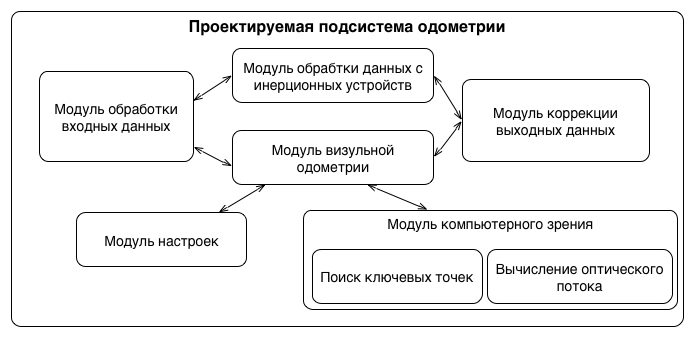
\includegraphics[width=0.8\linewidth]{pics/achitecture.png}}
\caption{Структура компонентов.}
\label{pic:acrhitec}
\end{figure}

\textbf{Назначение модулей}

\begin{itemize}
\item \textbf{Модуль обработки входных данных} - нормализует входные данные и аккумулирует их, в случае слишком высокой частоты их поступления.
\item \textbf{Модуль обработки выходных данных} - сравниевает данные, полученные независимо в модуле визуальной одометрии и в модуле обработки данных с ИИУ, и принимает решение об их корректности на основе определенных сигнальных показателей (см. пункт~\ref{item:outputCorrect}).
\item \textbf{Модуль визуальной одометрии} – вычисляет перемещения на основе видеоряда. Для обработки видео использует модуль компьютерного зрения. 
\item \textbf{Модуль компьютерного зрения} – реализует стандартные алгоритмы компютеного зрения, такие как вычисление оптического потока, поиск опорных точек на изображении, трансформация и измениние изображений.
\item \textbf{Модуль одометрии на основе инерционных устроств} – производит расчеты перемещения обхекта на основе полученных данныз с гироскопов и акселерометров.
\item \textbf{Модуль настроек} - содержит в себе данные об используемом оборудовании и его характеристиках. Эти данные используются в модулях одометрии. 
\end{itemize}

\paragraph{Описание процессов}
В ходе работы всей подсистемы протекает множество процессов по обработке и преобразованию информации. Выделим ключевые из них.

\textbf{Визуальная одометрия.}

В данной работе делается упор на создание визуальной одометрии на основе одной бытовой камеры и относительно слабых вычислительных устройств. Такое решение требует соблюдения двух условий, которые приемлемы при создании большинства современных мобильных роботов:
\begin{enumerate}
\item перемещение происходит по земле или другой горизонтальной плоскости;
\item камера жестко закреплена относительно самого носителя.
\end{enumerate}

При соблюдении этих условий работу визуальной одометрии можно описать в 8 шагов\cite{visaulOdometryMy}.
\begin{enumerate}
\item Исправление изображения для исключения искажения линз.
\item Вычисление оптического потока для кадра.
\item Проверка полученных векторов смещения, исключение движущихся в кадре объектов, исключение ошибочных векторов.
\item Разделение всего оптического потока на две части: «наземную» и «небесную».
\item В «небесной» части перейти к цилиндрической системе координат и высчитать угол поворота относительно двух последних кадров, определяя тем самым угол поворота $\theta$.
\item В «наземной» части выделить векторы $(u,v)$ из оптического потока  и вычислить перемещение в плоскости x-y , получив вектор $(x, y)$.
\item Прибавить $(x, y, \theta)$ к изначальному положению объекта $(X, Y, \Theta)$, получив новое положение объекта.
\item Перейти к шагу 1 для следующего кадра. Периодически обновлять ключевые точки.
\end{enumerate}
	
В общем виде процесс вычисления оптического потока представлен на рисунке~\ref{pic:visOdometryProc}.

\begin{figure}[!htb]
\center{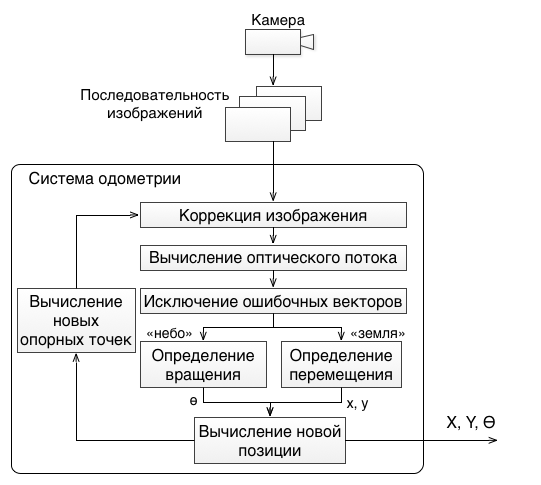
\includegraphics[width=0.8\linewidth]{pics/visualOdometryProcess.png}}
\caption{Графическое представление процесса визуальной одометрии}
\label{pic:visOdometryProc}
\end{figure}

\textbf{Обработка данных с инерционных измерительных устроств.}

Обработка данных с инерционных устройств представляет собой несколько операций интегрирования полученных данных. 
Рассмотрим переход от ускорений к перемещению.

Пусть на выходе акселерометра снимаются ускорения $Z_a$, $Y_a$ и $Z_a$, которые показывают ускрения по осям $X$, $Y$, $Z$.

Как мы знаем из курса физики, $ \int_a^b a(t)dt = V(t)+C $.
В то же время $ \int_a^b V(t)dt = S(t)+C $. Таким образом получаем:
$$
\iint_a^b a(t)dt = \int_a^b V(t) + C_v = S(t) + C_v \cdot t + C_s 
$$.

Так как $С_s$ в нашем случае, это начальное положение носителя, то его мы принимаем = 0. Отсюда получаем формулу:
$$
\iint_a^b a(t)dt = \int_a^b V(t) + C_v = S(t) + C_v \cdot t .
$$

Однако все упрощается, если период замеров настолько мал, что ускорение можно считать равномерным. Тогда формулы преобретают следующий вид:
$$ V_t = V_{t-1} + a_t \cdot t$$
$$ S_t = S_{t-1} + V_t \cdot t $$

Графически это можно выразить тремя графиками (рис.~\ref{pic:integral}): показывающими рассчитанное значения пермещения и сокрости в зависимости от времени. 

\begin{figure}[!htb]
\center{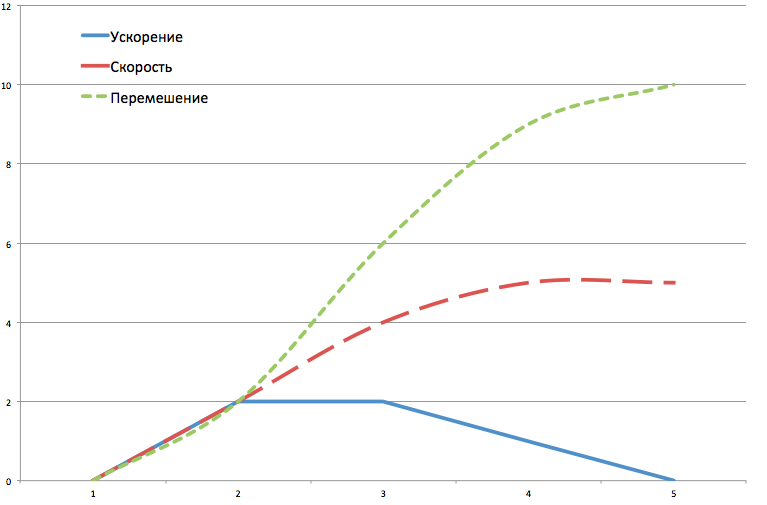
\includegraphics[width=0.8\linewidth]{pics/integrals.png}}
\caption{Пример интегрирования ускорения для получения перемещения}
\label{pic:integral}
\end{figure}


Производя подобные математические вычисления для координат $X$ и 
$Y$ получаем перемещения по этим координатам. Причем мы можем опускать финальную константу интегрирования, так как нам необходимо определить не пройденный путь от начала движения, а именно путь, пройденный за последнний временной отрезок. 

Аналогично обрабатываются данные с акселерометров, с одинм лишь отличием - акселерометры могут предоставлять сразу угловую скорость, что позволяет производить лишь одно интегрирование.


\paragraph{Математическое обеспечение}\label{math}

В рамках данной работы многие процессы основываются на фундаментальных исследованиях в области компьютерного зрения и обработки изображений. Далее рассматриваются основные из них.

\textbf{Поиск ключевых точек}

Есть много видов местных ключевых точек, которые можно отслеживать. Для начала стоит рассмотреть что из себя представляет ключевая точка сама по себе (ключевая особенность изображения). Очевидно, что если мы выбираем точку на большой однотонной стене, то будет не легко найти, что же точку в следующем кадре из видео.

Если все точки на стене могут быть одинаковыми или даже очень похожи, то у нас будет мало шансов отслеживания этой точки в последующих кадрах. С другой стороны, если мы выберем точку, которая является уникальной, то у нас будут довольно хорошие шансы снова найти эту точку. На практике, точка или черта, которая мы выбираем в качестве клюевой должны быть уникальным или почти уникальны, и должна быть параметризуемой таким образом, чтобы ее можно было отличить от других точек на изображении.

Возвращаясь к нашей аналогии с большой пустой стеной, мы могли бы попытаться искать точки, которые имеют некоторые значительные изменения в окрестности, например, большую производную. На практике оказывается, что этого не достаточно. Точка, в которой большое значение производной, может находиться на какой-то линии, но все точки на этой линии будут иметь такую же или близкую производную.

Однако, если высокие значения производные наблюдаются в двух ортогональных направлениях, то можно надеяться, что эта точка будет уникальной. По этой причине, такие особенности на изображении называются углами. Очевидно, углы - не края - это точки, которые содержат достаточно информации, чтобы ее нашли на последующих кадрах.

Определение углов опирается на матрице производных второго порядка 
$(\partial^2 x, \partial^2 y, \partial x \partial y)$ интенсивностей изображения. Эта терминология происходит от матрицы Гессе вокруг точки, которая определяется в двух измерениях следующим образом:

$$ 
H(p) = 
\begin{bmatrix} 
	\frac{\partial^2 I}{\partial x^2} & \frac{\partial^2 I}{\partial x \partial y}  \\ 
 	 \frac{\partial^2 I}{\partial x \partial y} & \frac{\partial^2 I}{\partial y^2} 
\end{bmatrix}
$$

Такие углы, по определению Харриса, места на изображении, где автокорреляционная матрица вторых производных имеет два больших собственных значения. По сути, это означает, что есть текстуры или грани , идущие, по крайней мере, в двух отдельных направлениях, сосредоточенные вокруг такой точки, так же, как реальные углы имеют по крайней мере два ребра, сходящихся в точку. Использование вторых производных позволяет точно определить особенности, потому что они не отвечают единым градиентами(так как при первой производной равной константе, вторая будет равна нулю). Это определение имеет дополнительное преимущество, в том, что когда мы рассматриваем только собственных значений автокорреляционной матрицы, мы рассматриваем величины, инвариантные также к вращению, что является важным, потому что объекты, которые мы отслеживаем могут вращаться, а также перемещаться. Следует также отметить, что эти два собственных значения делают больше, чем просто определяют, является ли точка перспективной для обслеживания - они также обеспечивают идентифицирующую роль для точки.

В используемом в данной работе пакете компьютерного зрения используется функция  $cvGoodFeaturesToTrack()$.
\begin{verbatim}
void cvGoodFeaturesToTrack(
        const CvArr* image,
        CvArr* eigImage, CvArr* tempImage,
        CvPoint2D32f* corners,
        int* cornerCount,
        double qualityLevel,
        double minDistance,
        const CvArr* mask=NULL,
        int blockSize=3,
        int useHarris=0,
        double k=0.04 
);
\end{verbatim}
Эта функция вычисляет воторые производные для точек и их собственные значения. Результатом работы функции является список точек, которые являются хорошими кандидатами для ключевых точек.

\textbf{Оптический поток}

Задача вычисления оптического потока можно сформулировать следующим образом: оценить движение между двумя кадрами не имея никакой информации о происходящем, кроме самих кадров\cite{OpenCVBook}. 

Вычисля оптический поток, мы можем связать для каждого пикселя определить некий ветктор смешения, которые будут показывать куда переместился пиксель между предыдущим кадром и текущим кадром. Такой  подход обычно называют плотным оптическим потоком, который определяет перемещение каждого пикселя. Метод Хорн-Шунка (Horn-Schunck) вычисляет именно такой оптический поток. В его основе лежит один, казалось бы, простой принцип - просто пытаться найти наиболее похожий пиксель на следующем кадре в пределах какого-то окна вокруг исходного пикселя.

На практике расчет плотного оптического потока затруднителен. Рассмотрим движение белого листа бумаги. Многие из белых пикселей в предыдущем кадре просто остаются белыми на следующих. Изменения будут лишь на границах листа, и то, только вокруг гарниц перпендикулярных движению. В результате необходимо прибегать к различным математическим приемам, что сказывается на увеличении ресурсоемкости операции в целом. 

Это приводит нас к альтернативному варианту, выборочный оптического потока. Алгоритмы такого рода опираются на некоторые средства определения заранее подмножество точек, которые должны быть отслежены. Если эти точки имеют определенные свойства, такие как свойства ключевых особенностей, обсуждаемые ранее, тогда отслеживая будет относительно точным и надежными. Для многих практических случаев, вычислительная стоимость выборочного оптичкского потока намного меньше, чем у плотного оптического потока, поэтому последнему отводится только академический интерес.

Рассмотрим наиболее популярный метод вычисления выборочного оптического потока - метод Лукаса-Канаде (Lucas-Kanade). Этот метод также имеет реализацию, которая работает с пирамидами изображений, что позволяет нам отслеживать быстрые движения. В данной работе используется именно он, так как он обладает наиболее низкой вычислительной сложностью. 

{\large \textit{\textbf{Метод Лукаса-Канаде}}}
\label{label:lucas-kanade-math}
Метод (алгоритм) Лукаса - Канаде (ЛК) создавался в 1981 году и первоначально задумывался для вычисления плотного оптического потока. Тем не менее, Алгоритм работал и с любым количеством точек для отлеживания, что позволило использовать его в столь важных выборочных оптических потоках. 

Алгоритм ЛК может быть применен для определнного числа точек, потому что он опирается только на локальной информации о точке, которая является производной в некотором маленьком окне вокруг каждой из ключевых точек. Недостатком использования небольших локальных окон в ЛК является то, что большие смещения могут перемещать точки за пределы таких локального окон, что приведет к невозможности их нахождения. Эта проблема привела к разработке "пирамидальной" версии алгоритма, которая составляет пирамиду из нескольких копий изображения разного размера, после чего вычисляет оптический поток, начиная с самого высокого уровня в пирамиде изображений, постепенно опускаясь по уровням для более высокой точности. 

\begin{figure}[!htb]
\center{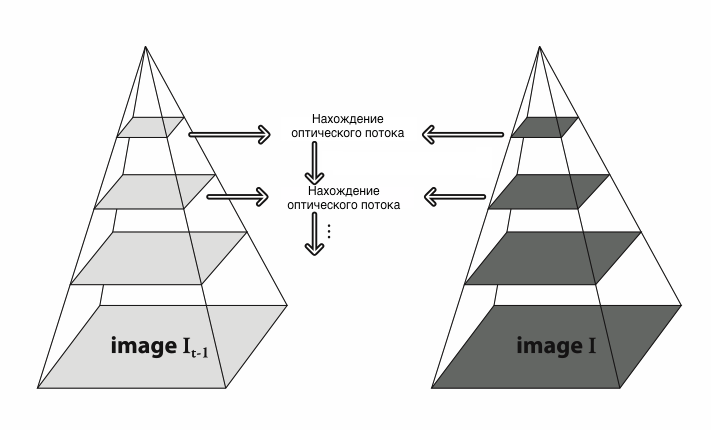
\includegraphics[width=0.8\linewidth]{pics/pyrLK.png}}
\caption{Графическое представление работы "пирамидальной" версии алгоритма ЛК}
\label{pic:pyrLK}
\end{figure}

\textbf{Принцип работы алгоритма}

Основная идея алгоритма ЛК основывается на трех предположениях. 
\begin{enumerate}
\item \textit{Яркость постояна.} Предполагается, что пиксель не меняет внешний вид, переходя от кадра к кадру. Для изображений в градациях серого (для случая с цветными изображениями есть более строгое допущение, но оно сводится к этому) это означает, что яркость пикселя не меняется, при его отслеживании от кадра к кадру. 
\item \textit{Малые сдвиги}. Изображение двигается медленно во времени. На практике это означает, что объект от кадра к кадру сдвигается незанчительно.
\item \textit{Пространственная когерентность.} Соседние точки в кадре принадлежат к одной и той же поверхности и имеют аналогичные смещения.
\end{enumerate}

Из первого допущения следует:
$$
f(x, t) \equiv I(x(t), t) = I(x(t+dt), t + dt)
$$

Отсюда следует, что интенсивность отслеживаиваемых пикселей не измененяется с течением времени:
$$
\frac{\partial f(x)}{\partial t} = 0
$$

Второе предположение, по существу, означает, что движения от кадра к кадру крайне малы. Другими словами, мы можем рассматривать это изменение как аппроксимацию производной от интенсивности по времени. Чтобы понять последствия этого предположения, рассмотрим сначала случай одного пространственного измерения.
Запишем уравнение яркости $F(x,t)$ с учетом зависимости $x$ от $t$ и применим правило частного дифференцирования:
$$
\underbrace{\frac{\partial I }{\partial x} \Bigr|_t}_{I_x} 
\underbrace{\left( \frac{\partial x }{\partial t} \right)}_{V} + 
\underbrace{\frac{\partial I }{\partial t} \Bigr|_{x(t)}}_{I_t} =
 0,
$$

где $I_x$ является пространственной производной по первому изображению, $I_t$ это производная между изображениями в течение долгого времени, и $V$ -скорость, которую мы ищем. Таким образом, мы приходим к простому уравнению для скорости оптического потока в простой одномерной случае:

$$ V = \frac{I_t}{I_x} $$

Рассмотрим стандартную задачу в одномерном случае. На рисунке~\ref{pic:OptFlow1D} представлена ее графическая иллюстрация. Кривая $I(x, t)$ изображает некую грань, слева от которой значения интенсивности высоки, а справа - низкие. Необходимо определить как сдвинулась это грань на следующем кадре. 

\begin{figure}[!htb]
\center{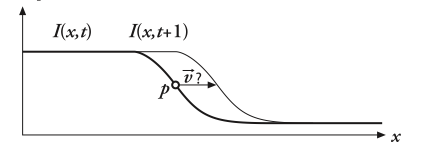
\includegraphics[width=0.8\linewidth]{pics/optFlow1D.png}}
\caption{Графическое представление задачи нахождения оптического потока в одномерном случае.}
\label{pic:OptFlow1D}
\end{figure}

На рисунке~\ref{pic:OptFlow1DSolve} показано как можно решить такую задачу. При учете двух первых предположений  получим следующее:
$$
I_x = \frac{\partial I}{\partial x} \Bigr|_t \; и \;
I_t = \frac{\partial I}{\partial t} \Bigr|_{x=p} \Rightarrow 
\vec{V} \approx - \frac{I_t}{I_x}
$$
\begin{figure}[!htb]
\center{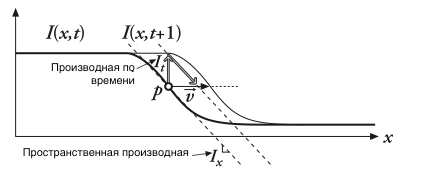
\includegraphics[width=0.8\linewidth]{pics/OptFlow1DSolve.png}}
\caption{Графическое представление решения задачи нахождения оптического потока в одномерном случае.}
\label{pic:OptFlow1DSolve}
\end{figure}

Теперь рассмотрим двумерный случай. Будем обозначть $u_y$ скорость вдоль оси $Y$, а $u_x$ -вдоль $X$:
$$ I_xu +I_yv+I_t = 0 \equiv 
\frac{\partial I}{\partial t} + 
u_x \cdot \frac{\partial I}{\partial x} + 
u_y \cdot \frac{\partial I}{\partial y} = 0 
$$

Полученное уравнение, говорит нам о том, что сумма частных производных должны быть равна нулю. Но вознакает проблема - уравнение у нас одно, а неизвестных в нем два: $u_x$ и $u_y$.

Воспользовавшись третьим предположением, о том, что соседние пиксели смещаются на одинаковое расстояние, запишем это же уравнение для окна 5х5 пикселей, получив 25 уравнений. Очевидно, что 3 допущение не всегда верно, поэтому в общем случае система не имеет решения поэтому перейдем к минимизации ошибки:

$$
E(u_x, u_y) = \sum \limits_{i,j} g(x_i, y_i) 
\left[ \frac{\partial I}{\partial t} + 
u_x \cdot \frac{\partial I}{\partial x} + 
u_y \cdot \frac{\partial I}{\partial y} \right]^2
$$

Здесь $g$ — это функция, определяющая весовые коэффициенты для пикселей. Самые распространенный вариант — двумерная гауссиана, которая дает наибольший вес центральному пикселю и все меньший по мере удаления от центра (см. рис.~\ref{pic:Gaussian2d}).

\begin{figure}[!htb]
\center{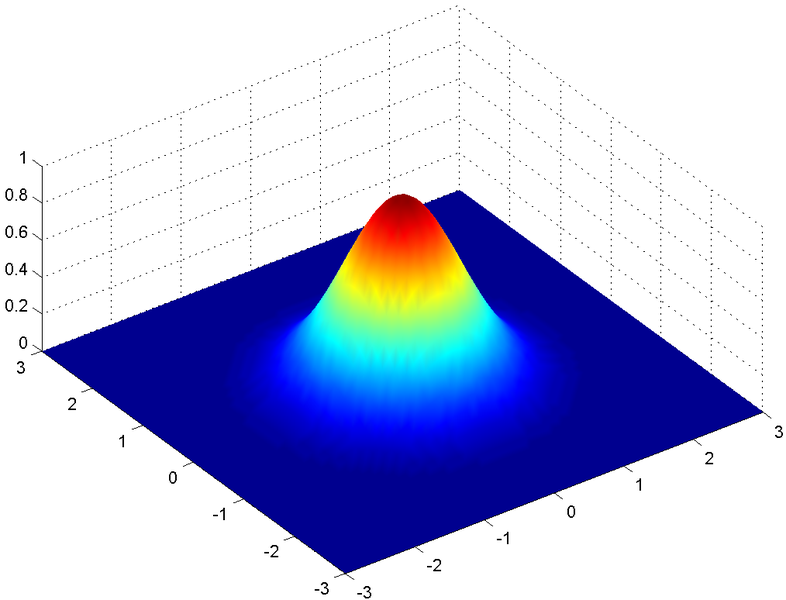
\includegraphics[width=0.8\linewidth]{pics/Gaussian2d.png}}
\caption{Двумерная гауссиана}
\label{pic:Gaussian2d}
\end{figure}

Чтобы найти минимум  $E(u_x, u_y)$ воспользуемся методом наименьших квадратов, найдем её частные производные по $u_x$ и $u_y$ и запишем в более компактной форме, приравням к 0:

$$
\frac{\partial E(u_x, u_y) }{\partial u_x} = 
\sum \limits_{i,j} g(x_i, y_i) 
\left[
u_x \left( \frac{\partial I}{\partial x} \right)^2 +
	u_y \frac{\partial I}{\partial y}\frac{\partial I}{\partial x} +
	\frac{\partial I}{\partial x}\frac{\partial I}{\partial t}
\right] = 0
$$

$$
\frac{\partial E(u_x, u_y) }{\partial u_y} = 
\sum \limits_{i,j} g(x_i, y_i) 
\left[
	u_x \frac{\partial I}{\partial y}\frac{\partial I}{\partial x} +
	u_y \left( \frac{\partial I}{\partial y} \right)^2 +
	\frac{\partial I}{\partial x}\frac{\partial I}{\partial t}
\right] = 0
$$

Перепишем эти два уравнения в матричной форме:
$$ M \vec{u} = \vec{b}$$

Где: 
$$ M = 
\left[ 	
\begin{array}{cc}
	\sum \limits_{i,j} g(x_i, y_i) 
		\left( \frac{\partial I}{\partial x} \right)^2 
	& \sum \limits_{i,j} g(x_i, y_i) 
			\frac{\partial I}{\partial x} 										\frac{\partial I}{\partial y} 
	\\ 
	\sum \limits_{i,j} g(x_i, y_i) 
			\frac{\partial I}{\partial x} 										\frac{\partial I}{\partial y} 
	& \sum \limits_{i,j} g(x_i, y_i)
		\left( \frac{\partial I}{\partial y} \right)^2 
\end{array} 
\right]
$$

$$
\vec{b} = -
\left[ 	
\begin{array}{c}
\sum \limits_{i,j} g(x_i, y_i) 
			\frac{\partial I}{\partial t} 										\frac{\partial I}{\partial x}  \\ 
\sum \limits_{i,j} g(x_i, y_i) 
			\frac{\partial I}{\partial t} 										\frac{\partial I}{\partial y}
\end{array} 
\right]
$$

$$
\vec{u} = 
\left[ 	
\begin{array}{c}
  u_x\\ 
	u_y
\end{array} 
\right]
$$

Если матрица М обратима (имеет ранг 2), можем вычислить $u_x$ и $u_y$ , которые минимизируют ошибку $E$\cite{habrOpticalFlowAbout}:
$$
\widehat{u} = M^{-1} \cdot \vec{b}
$$

\textbf{Калибровка камеры}
Еще одиним математическим аспектом данной работы является калибровка камеры. 

\textit{\textbf{Калибровка камеры}} — это задача получения внутренних и внешних параметров камеры по имеющимся фотографиям или видео, отснятым ей\cite{wikiCalibrate}.

Рассмотрим простейшую модель камеры, камеры-обскуры. В этой простой модели, свет рассматривается в качестве потка от сцены или удаленного объекта, но только один луч попадает из любой конкретный точки этого объекта. Все эти точки проецируются на матрицу камеры или другую поверхность изображения. В результате, изображение на этой плоскости изображения всегда в фокусе, а масштаб изображения относительной его раельного размера определяется одним параметром камеры -  ее фокусным расстоянием. На рисунке~\ref{pic:cameraModel} схематично показана рассматриваемая модель камеры\cite{OpenCVBook}. 

\begin{figure}[!htb]
\center{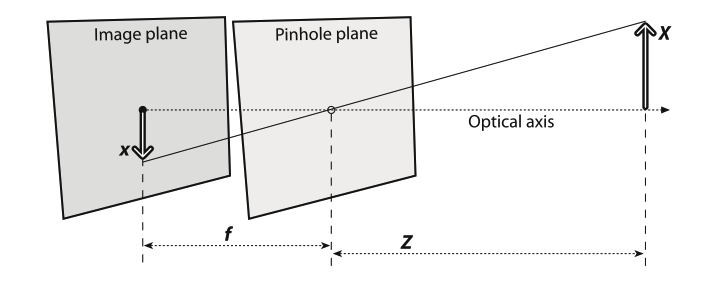
\includegraphics[width=0.8\linewidth]{pics/cameraModel.png}}
\caption{Модель камеры-обскуры}
\label{pic:cameraModel}
\end{figure}

Из изображения видно, что, на основе подобия треугольников, $-x/f = X/Z$:
$$	-x = f \cdot \frac{X}{Z} $$

Учитывая тот факт, что главная оптическая ось пересекает плоскость изображения не в координате $(0,0)$, в координате $с$ получим:

\begin{equation}
\label{formula:focus}
-x = f \cdot \frac{X}{Z} + с
\end{equation}

Далее будем рассматривать именно цифровые камеры с ПЗС-матрицами. У данных камер есть одна особенность - пиксели матрицы не квадратной формы из-за технологических условий изготовления. Учитывая этот факт, распишем уравнение (\ref{formula:focus}) для координат $x$ и $y$:

$$ u = f \cdot s_u \cdot \frac{X}{Z} + c_u $$
$$ v = f \cdot s_v \cdot \frac{X}{Z} + c_v $$

где $s_u$ и $s_v$ - коэффициенты формы пикселя.
Запишем эти уравнения в матричной форме:

\begin{equation}
\label{formula:matrixProection}
q = \frac{1}{Z} \cdot M \cdot Q
\end{equation}

где 
$Q_i = 
\left( 
\begin{array}{c}
X_i \\ 
Y_i \\ 
Z_i
\end{array} 
\right)$ - координаты точки во внешней системе координат,

$q_i = 
\left( 
\begin{array}{c}
u_i \\ 
v_i \\ 
1
\end{array} 
\right)$ - координаты проекции точки,

$M = 
\left( 
\begin{array}{ccc}
f_u & 0 & c_u \\ 
0 & f_v & c_v \\ 
0 & 0 & 1
\end{array} 
\right)$ - матрица проекции.

Теперь ведем линзу в модель камеры. Линза так же вносит искажения, природа происхождения которых показана на рисунке~\ref{pic:distorb}.

\begin{figure}[!htb]
\center{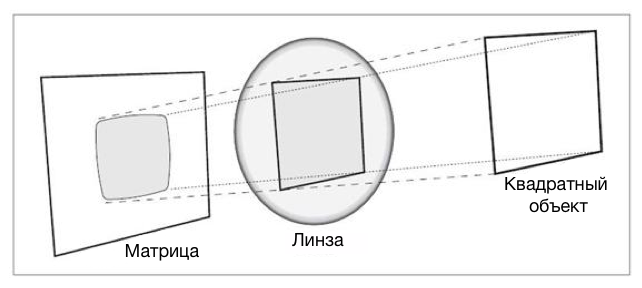
\includegraphics[width=0.8\linewidth]{pics/distorb.png}}
\caption{Искажения изображения, вносимые линзой}
\label{pic:distorb}
\end{figure}

Данный вид искажения называется радиальным. Он учитывается следующим образом:
$$
u_{corrected} = u \cdot (1 + k_1 \cdot r^2  + k_2 \cdot r^4 )
$$
$$
v_{corrected} = v \cdot (1 + k_1 \cdot r^2  + k_2 \cdot r^4 )
$$
Здесь $r$ – расстояние от точки пересечения главной оптической осью матрицы до точки проекции; $k1, k2$ – коэффициенты радиального искажения.

С учетом этих искажений формула \ref{formula:matrixProection} принимает вид:
\begin{equation}
\label{formula:matrixProection2}
q = \frac{1}{Z} \cdot \left( 
\begin{array}{ccc}
	\lambda & 0 & 0 \\ 
	0 & \lambda & 0 \\ 
	0 & 0 & 1
\end{array} 
\right) 
 \cdot M \cdot Q
\end{equation}
где $\lambda$ - корректирующая функция:
$$ \lambda = 1 + k_1 \cdot r^2  + k_2 \cdot r^4 $$

Кроме радиального искажения существует ещё тангенциальное. Оно возникает из-за того, что плоскость матрицы не перпендикулярна главной оптической оси. Но оно очень мало, и его можно не учитывать. 

При установке камеры тоже появляются погрешности – учтем их в модели.

Погрешности ориентации:
$$R_z(\theta) = 
\left( 
	\begin{array}{ccc}
	\cos (\theta ) & \sin (\theta ) & 0 \\ 
	- \sin (\theta ) & \cos (\theta ) & 0 \\ 
	0 & 0 & 1
\end{array} 
\right) 
$$

$$
R_x(\psi ) = 
\left( 
	\begin{array}{ccc}
	1  & 0 & 0 \\ 
	0 & \cos (\psi ) & \sin (\psi ) \\ 
	0 & - \sin (\psi ) & \cos (\psi ) \\ 
\end{array} 
\right) 
$$

$$
R_y(\varphi ) = 
\left( 
	\begin{array}{ccc}
	\cos (\varphi ) & 0 & - \sin ( \varphi )  \\ 
	0 & 1 & 0 \\ 
	\sin (\varphi ) & 0 & \cos (\varphi ) \\ 
\end{array} 
\right) 
$$

Результирующая матрица вращения камеры вокруг требуемой системы координат:

$$ R(\psi , \varphi , \theta ) = R_x(\psi ) \cdot R_y(\varphi ) \cdot R_z(\theta ) $$

, где $ \theta , \varphi , \psi $ - углы Эйлера.

Вектор смещения камеры относительно требуемой системы координат:
$$ 
T = 
\left( 
\begin{array}{c}
t_x \\ 
t_y \\ 
t_z
\end{array} 
\right) 
$$ 

Теперь модель камеры с учётом радиального искажения и погрешностей установки выглядит так\cite{cameraCalibrate}
$$
q = \frac{1}{Z} \cdot \left( 
\begin{array}{ccc}
	\lambda & 0 & 0 \\ 
	0 & \lambda & 0 \\ 
	0 & 0 & 1
\end{array} 
\right) 
 \cdot M \cdot R \cdot (Q + T)
$$

\subsubsection{Разработка формата и структуры данных}
В ходе функционирования подсистемы информация поступает на ее вход, получается на ее выходе, и передается между модулями внутри системы. 
При этом эта информация носит разные характер и смысл. Так как подсистема носит сугубо программный характер, то все потоки даных реализуются только программными средствами, в виде структур данных. Сетевые технологии не накладывают никаких ограничений на форматы информационных структур. 
Ниже дано описание основных форматов обмена информацией.

\begin{itemize}
\item \textbf{Видео (вход)}. Видео подается на вход системы покадрово, в связи с этим алгоритм кодирования и сжатия видео не существеннен, так как задача сформировать следующий кадр в его полном объеме ложиться на вызывающую стороную. По сути, каждый кадр представляет собой 1 картинку в формате JPEG, что проще всего представать матрицей, размер которой соответствует размеру кадра, а ее элементами являются структуры данных, хранящие информацию о каналах изображения. 

\item \textbf{Ускорения по трем осям (вход)}. Данные подаваемые с акселерометров или одного, трехосевого акселерометра. Данные имеют цифровое представления, дробное. 

\item \textbf{Угловое ускорение по трем осям (вход)}. Данные подаваемые с гироскопов или одного, трехосевого гиросокопа. Данные имеют цифровое представления, дробное. 

\item \textbf{Текущие координаты и угол поворота (выход)}. Высчитанное на текущей итерации положение объекта. Две координаты $X$ и $Y$ представляют собой целые числа. Угол поворота  $\alpha$- дробное число. Аналогиным образом можно представлять информацию о смещениях, полученных на текущей итерации. 

\item \textbf{Информационный обмен между модулем визуальной одометрии и модулем компьютерного зрения}. Данный информационых обмен происходит два раза за итерацию: для нахождения ключевых точек на кадре и для вычисления оптического потока. При этом в разных случаях содержание информационных сообщений будет разное.
	\begin{itemize}
	\item Нахождение ключевых точек - от модуля визуальной одометрии поступает изображение, являющееся кадром. Пресдставляет собой матрицу, размер которой соответствует размеру кадра, а ее элементами являются структуры данных, хранящие информацию о каналах изображения. В ответ модуль компьютерного зрения возвращает список точек в формате ${x, y}$, где $x$ и $y$ - позиция пикселя на изображении при начале отсчета в левом верхнем углу. 
	
	\item Вычисление оптического потока - от модуля визуальной одометрии поступает два изображения (текущий и предыдущий кадры)и список ключевых точек. Представление соответствует описаному ранее. В ответ модуль компьютерного зрения возвращает два списка: список смещений, представляющий собой список пар $\triangle x, \triangle y$, и вектор ошибок, состоящий из 0 и 1 - 1 означает, что соотвествующая ключевая точка не была найдена на втором изображении и вектор смещения найден ошибочно или не найден вообще. 
	
	\end{itemize}
\end{itemize}

\subsubsection{Разработка алгоритмов обработки информации}
\paragraph{Общий алгоритм работы}
\paragraph{Алгоритм вычисления оптического потока}
\paragraph{Алгоритм обработки данных с ИИУ}
\paragraph{Алгоритм сопоставления и корректировки выходных данных}


\newpage
\section{Технологическая часть}

\subsection{Руководство по интеграции и настройке подсистемы}
Одной из целей при создании ПОАПО являлось создание удобного и простого в интеграции с другими системами модуля для автономной навигации объектов. Руководствуюясь этой целью, процесс установки и настройки был максимально упрощен. 
Для корректной работы подсистемы необходимо использовать оборудование, указанное в техническом задании к системе, а именно:
\begin{itemize}
\item требования к цифровой камере:
	\begin{itemize}
	\item разрешение не ниже 1 Мп;
	\item интерфейс соединения со скоростью не ниже 12 Мбит/с;
	\item жесткое крепление на объекте;
	\end{itemize}
\item Требования к инерциальному измерительному устройству 
 	\begin{itemize}
 	\item трехосевой гироскоп с диапазоном измерения до 2000 $^\circ$/с и точностью не ниже, чем 0,2$^\circ$ на 1 $^\circ$/с;
	\item акселерометр с тремя степенями свободы и дипазоном измерения $\pm10g$.
 	\end{itemize}
\end{itemize}

Вторым этапом интеграции является жесткое закрепление камеры и ИИУ на подвижном объекте, перемещения которого и предполагается расчитывать. Камеру необходимо расположить по направлению движения и так, чтобы в кадре 70\% изображения занимала горизонтальная поверхность, по которой происходит движение, и 30\% кадра занимали объекты, расположенные над линией горизонта.  

Далее нужно провести каллибровку камеры для выявления внутренних и внешних параметров камеры. С теоретической точки зрения данных процесс описан в пункте~\ref{part:calibrateCamera}. На практике процесс является более простым и заключается в виксации <<специального изображения>> камерой и последующем анализе полученного изображения. Данный метод калибровки называется <<новым гибким методом калибровки камеры>> и был предложен Zhengyou Zhang\cite{Zhang}. Как правило в качестве <<специального изображения>> используется изображения шахмотной доски. Суть методоа заключается в нахождении углов такой доски и подбору внутренних параметров камеры таким образом, чтобы на изображении эти углы выстраивались в прямые линии. Для корректного опредления параметров камеры желательно получить как можно больше изображений такой доски под разными углами. Схематично данный процесс отображен на рисунке~\ref{pic:calibrationMan}.

\begin{figure}[!h]
\center{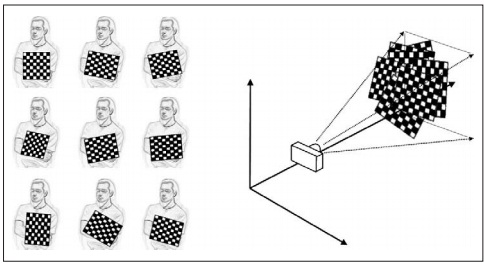
\includegraphics[width=0.8\linewidth]{pics/calibrationMan.png}}
\caption{Процесс гибкого метода калбровка камеры.}
\label{pic:calibrationMan}
\end{figure}

В то же время, данный метод можно применять для вычисления матрицы трасформации изображений. Рассмотрим рисунок~\ref{pic:perspectiveTranform}. Если фиксирвоать изображения шахматной доски в плоскости левой фигуры, то при удалении искажений мы получим изображение строго перпендикулярное камере. В визуальной одометрии наоборот необходимо отобразить все клюевые точки в плоскости пола. Таким образом, получив матрицу изменения изображения, транспанируем ее и будем применять для нормализованных изображений с целью опрделить реальное положение ключевых точек кадра на плоскости перемещения. 

\begin{figure}[!h]
\center{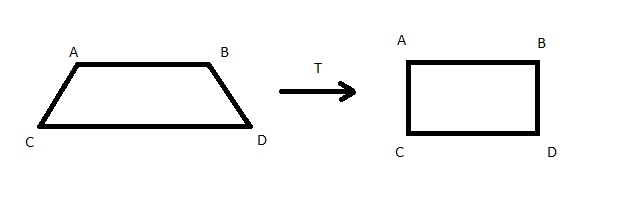
\includegraphics[width=0.8\linewidth]{pics/perspectiveTransform.png}}
\caption{Принцип перспективного преобразования изображений.}
\label{pic:perspectiveTranform}
\end{figure}

После устновки необходимого оборудования и его калибровки необходимо согласовать программный интерфейс подсистемы для корректного передачи видеоряда и данных с ИИУ. 
Подсистема ПАОПО предоставляет следующий API:

PutNewData


\subsection{Диаргамма взаимодейсвия компонентов}
В ходе работы подсистемы происходит взаимодейсвие ее модулей между собой и с внешними системами. Диаграмма последовательности такого взаимодейсвия показна на рисунке~\ref{pic:secquence}.

\afterpage{
\clearpage
%\thispagestyle{empty}
\begin{landscape}
\begin{center}
	\begin{figure}[H]
	\center{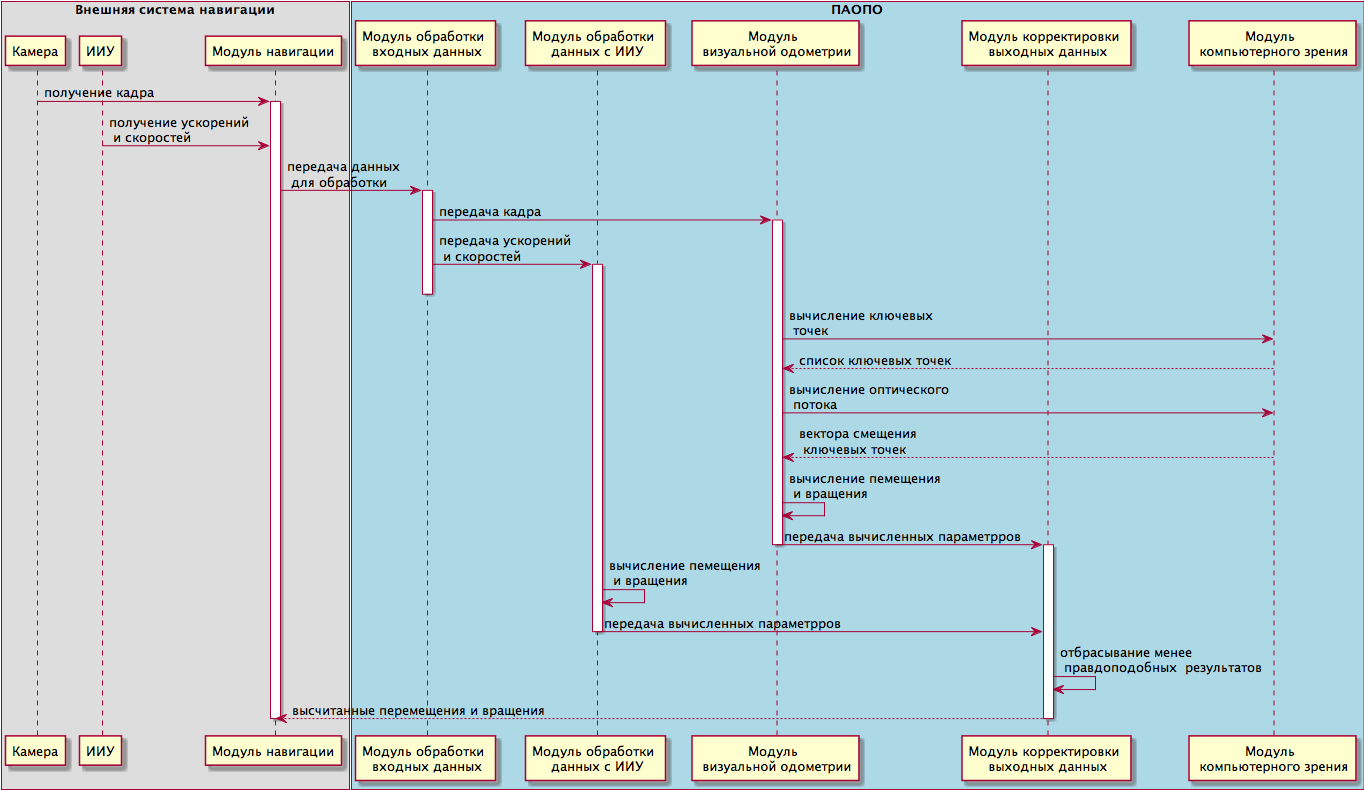
\includegraphics[width=1\linewidth]{pics/sec.png}}
	\caption{Диаграмма последовательности взаимодейсвия компонентов.}
	\label{pic:secquence}
	\end{figure}
\end{center}
\end{landscape}
\clearpage
}


\subsection{Диаграмма классов подсистемы}
При реализации прототипа рассматриваемой подсистемы был написан программный продукт на  языке Java в программном пакете JetBrains IDEA. В качестве модуля компьютерного зрения использовалась библиотека OpenCV (Open Computer Vision). 
В результате был получен программный продукт состоящий из нескольких классов, связанных между собой. Получившаяся диаграмма классов представлена на рисунке~\ref{pic:classDiagram}.


\begin{figure}[!htb]
\center{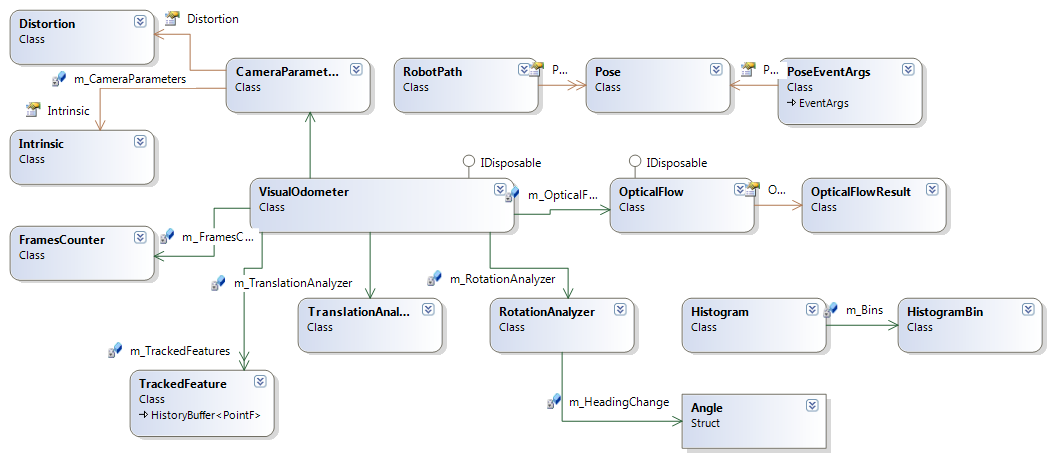
\includegraphics[width=0.9\linewidth]{pics/classDiagram.png}}
\caption{Диаграмма классов прототипа подсистемы.}
\label{pic:classDiagram}
\end{figure}
\newpage
\section{Исследовательская часть}
\subsection{Обоснование области исследования}
\textit{\textbf{Оптический поток (Optical flow)}} – технология, использующаяся в различных областях компьютерного зрения для определения сдвигов, сегментации, выделения объектов, компрессии видео и прочего. В специализированной литературе и глобальной сети Internet много вводных статей в эту технологию, в которых рассмотрены основные шаги для реализации оптического потока в своих проектах. Однако, при попытке реализовать оптический поток самостоятельно на основе полученной информации, такие реализации  работают очень плохо и сбоят при определении сдвигов уже порядка 1-2 пикселей.

В таких случаях следует обратиться к готовым реализациям этих методов. В настоящий момент наиболее развитой библиотекой компьютерного зрения является OpenCV\cite{wikiOpenCV}. Но в этой библиотеке реализовано множество способов вычисления оптического потока, у каждого из которых несколько параметров, которые как-то оказывают влияние на качество и скорость работы алгоритмов. 

В данной работе оптический поток играет ключевую роль, а время его вычисления занимает более половины времени работы всей системы. В связи с чем, в исследовательской части будут рассмотрены реализованные в OpenCV методы вычисления оптического потока, исследовано влияние их параметров на скорость работы алгоритмов, а так же оценено время работы каждого из методов при разных входных данных, приближенных к условиям работы разрабатываемой системы.

\subsection{Описание исследуемых методов}
\subsubsection{метод Лукаса-Канаде}
Метод Лукаса-Канаде является стандартным подходом к вычислению оптического потока, так как обладает достаточно низкой ресурсоемкостью и временем выполнения. В основном это достигается за счет вычисления не плотного оптического потока, а выборочного, для определенных точек изображения. Подробно этот алгоритм был рассмотрен в пункте \ref{label:lucas-kanade-math}. 

\subsubsection{метод Horn–Schunck}
Метод Horn–Schunck носит несколько более глобальный характер, чем метод Лукаса-Канаде. Он опирается на предположение о том, что на всем изображении оптический поток будет достаточно гладким.

Этот алгоритм был реализован в первых версиях OpenCV, но в последствии от него отказались по причине его плохой приспособленности к реальным видеопотокам. Данный метод упомянут только для ознакомления, в дальнейшем он не будет рассматриваться. 

\subsubsection{метод Farneback}
В данном методе предлагается аппроксимировать изменение интенсивности в окрестности с помощью квадратичной формы: $I = xAx + bx + c$ с симметричной матрицей $A$ (по сути, рассматривая разложение по Тейлору до первого члена, мы брали линейную аппроксимацию I = bx + c. используя указанное разложение мы увеличиваем точность аппроксимации.)
Если изображение сдвинулось в пределах этой окрестности, то 
$I_2 (x) = I_1 (x-d)$, подставив в квадратичное разложение и раскрываем скобки, получаем:

$$ A_2 = A_1 $$
$$ b_2 = b_1 - 2A_1d $$
$$ c_2 = d^TA_1d - b_1^Td + c_1 $$
Вычисляя значения $A, b, c$ на обеих картинках, получим избыточную систему относительно d. Более того, приближенное значение $d$ можно получить из второго уравнения: 
$$ d = -\frac{1}{2} \cdot A^{-1} \ cdot (b2 - b_1) $$

\subsubsection{метод SimpleFlow}
В основе метода SimpleFlow лежит следующая идея: если все равно нет возможности определять сдвиг больше чем размер окна, по которому мы искали производные, то можно просто в окне найти наиболее похожую точку. А для разрешения неоднозначность и для компенсации шумов учитывать, что поток непрерывный и в окрестности данной точки все точки имеют почти одинаковый сдвиг. Возникающие трудности с размером окна возможно решить за счет multi-scaling'а\footnote{итеративное вычисление оптического потока для уменьшенных изображений с целью определения больших сдвигов.}.

\subsubsection{метод Dual TV L1}
В ходе написания данной работы, 25 апреля 2014 года, была выпущена новая версия OpenCV 2.4.9, в которой был реализован еще одни метод вычисления оптического потока - Dual TV L1. 
К сожалению к этому моменту эксперимент был завершен и исследование еще и этого метода не представлялось возможным. 

\subsection{Проведение эксперимента}

Целью эксперимента было выявление зависимостей времени вычисления оптического потока разными методами от размера кадров и различных параметров этих методов.

\subsubsection{Методика проведения эксперимента}
Эксперимент проводился следующим образом.
Для анализа производительности каждым методом анализировался видеофайл длительностью 10 секунд и с частотой кадров - 30 кадров/сек. Итого оптический поток был высчитан для 299 кадров (для первого кадра не вычисляется). Размер кадра изменялся от 160*90 до 1280*720 пикселей с увеличением кадра в 2 раза на каждом тесте.

\subsubsection{Исходный код программы}
Для проведения эксперимента была написана программа на языке Java с использовании библиотеки JavaOpenCV. 

\begin{verbatim}
     1	public Mat onCameraFrame(CvCameraViewFrame inputFram
e) {
     2	   
     3	    mGray = inputFrame.gray();
     4	    Mat resizeImg = new Mat();
     5	
     6	    if (mPrevGray != null && !mPrevGray.empty()) {
     7	       
     8	        MatOfKeyPoint mKeyPoint = new MatOfKeyPoint(
);
     9	        FeatureDetector.create(FeatureDetector.HARRI
S).detect(mPrevGray, mKeyPoint);
    10	
    11	        ArrayList<Point> temp = new ArrayList<Point>
();
    12	        List<KeyPoint> keyPointsList = mKeyPoint.toL
ist();
    13	        for (int i = 0; i<keyPointsList.size(); i++)
    14	        {
    15	            temp.add(keyPointsList.get(i).pt);
    16	        }
    17	        MatOfPoint2f needs = new MatOfPoint2f();
    18	        needs.fromList(temp);
    19	        MatOfPoint2f result = new MatOfPoint2f();
    20	        MatOfByte status = new MatOfByte();
    21	        MatOfFloat err = new MatOfFloat();
    22	
    23	        calcOpticalFlowPyrLK(mPrevGray, mGray, needs
, result, status, err);
    24	
    25	    }
    26	
    27	    mPrevGray = mGray;
    28	    count++;
    29	
    30	return mGray;
    31	}

\end{verbatim}

\subsubsection{Тестовый стенд}
Сначала тестирование проводилось на настольном персональном компьютере со следующими характеристиками:

\begin{itemize}
\item процессор Intel Core i7 с тактовой частотой 3100МГц; 
\item 4ГБ оперативной памяти.
\end{itemize}

Однако при такой конфигурации оборудования отличия во времени выполнения на разных размерах кадра были незначительными, поэтому эксперимент был проведен на смартфоне LG Nexus 4 со следующими характеристиками:
\begin{itemize}
\item процессор Nvidia с тактовой частотой 1500МГц;
\item 2ГБ оперативной памяти.
\end{itemize}

\subsubsection{Результаты эксперимента}
Отпический поток высчитывался 3-мя методами: SimpleFlow, Farneback и Lucas-Kanade. Все эти три метода реализованы в библиотеке компьютерного зрения OpenCV и вначале вызывались со стандартными параметрами. Замерялось время вычисления ОП для всей видеопоследовательности. Результаты эксперимента представлены на рисунке~\ref{pic:compareMethods}.

\begin{figure}[!htb]
\center{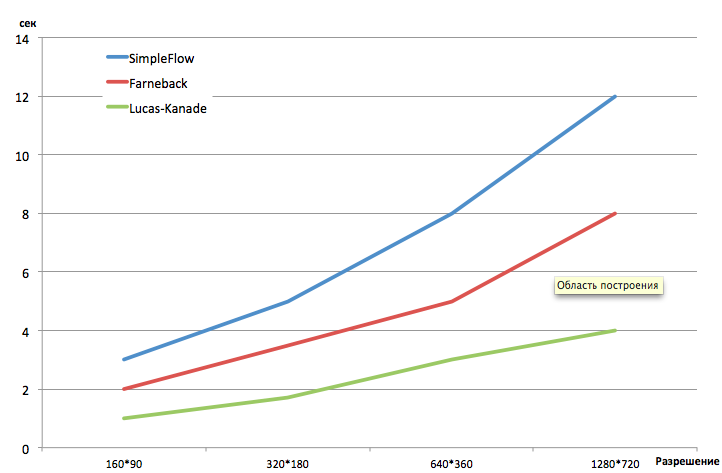
\includegraphics[width=0.8\linewidth]{pics/compareMethods.png}}
\caption{Сравнение времени выполнения методов вычисления оптического потока}
\label{pic:compareMethods}
\end{figure}

Из графика видно, что метод Лукаса-Канаде является самым быстрым, что обусловлено тем, что этим методом вычисляется лишь выборочный поток, а не плотный. 

Тем не менее, методы обладают рядом параметров, которые могут позволить увеличить их производительность. В связи с этим были проведено исследование их влияния на общее время вычисления оптического потока. 

\paragraph{Farneback}
Согласно документации OpenCV метод Farneback имеет следующие параметры.
\begin{itemize}
\item \textit{prev} – первое изображение.
\item \textit{next} – второе изображение.
\item \textit{flow} – вычисленный оптический поток в виде векторов. 
\item \textit{pyr--scale} – параметр, характеризующий коэф. уменьшения изображений при построении пирамиды. Стандартное значение - 0,5.
\item \textit{levels} – число уровне в пирамиде. Стандартное значение - 3.
\item \textit{winsize} – средний размер окна. Стандартное значение - 15.
\item \textit{iterations} – число итераций на каждом уровне пирамиды. Стандартное значение - 3.
\item \textit{poly--n} – число пикселей, используемых для идентификации ключевых точек. Стандартное значение - 5.
\item \textit{poly--sigma} – стандартное отклонение Гаусса, используемое для сглаживания производных. Стандартное значение - 1,1.
\end{itemize}

Очевидно, что первые три параметра изменять нельзя, кроме размера самих кадров, что мы и так делаем. 
На рисунке~\ref{pic:3FB_params} показано влияние других параметров на время вычисления оптического потока. 

\begin{figure}[!Htb]
\begin{minipage}[h]{0.47\linewidth}
\center{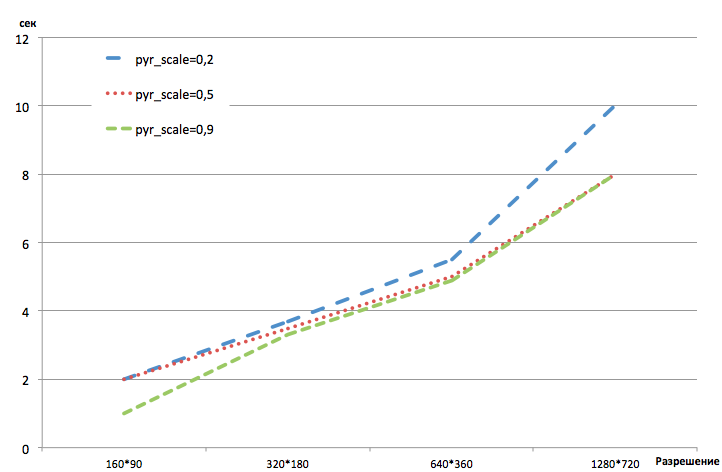
\includegraphics[width=1\linewidth]{pics/3FB_pyrscale.png}} a) \\
\end{minipage}
\hfill
\begin{minipage}[h]{0.47\linewidth}
\center{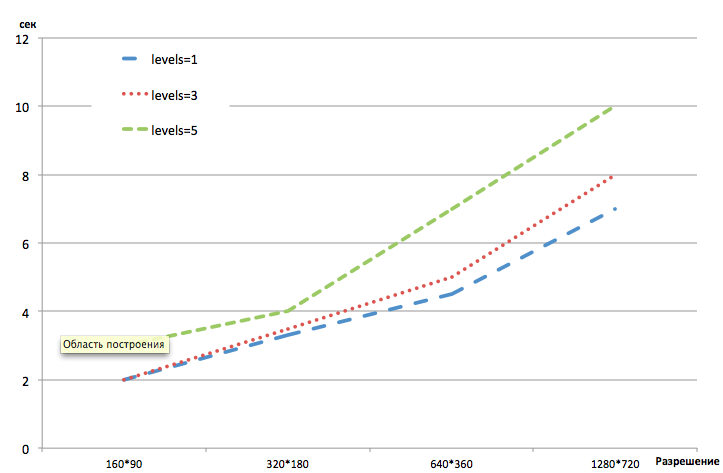
\includegraphics[width=1\linewidth]{pics/3FB_levels.png}} б)\\
\end{minipage}
\vfill
\begin{minipage}[h]{0.47\linewidth}
\center{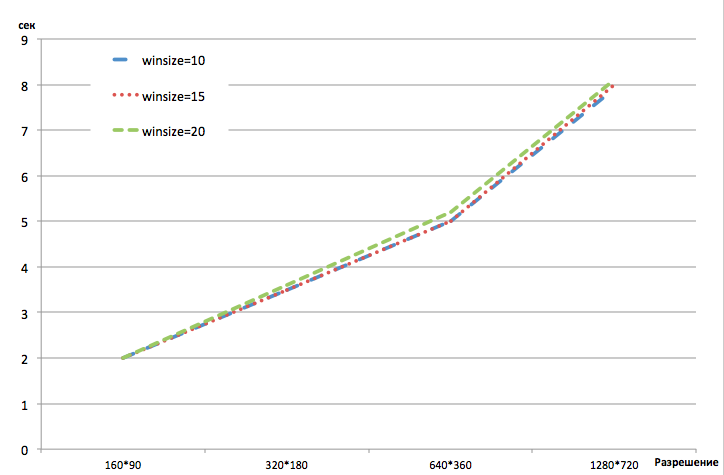
\includegraphics[width=1\linewidth]{pics/3FB_winsize.png}} в) \\
\end{minipage}
\hfill
\begin{minipage}[h]{0.47\linewidth}
\center{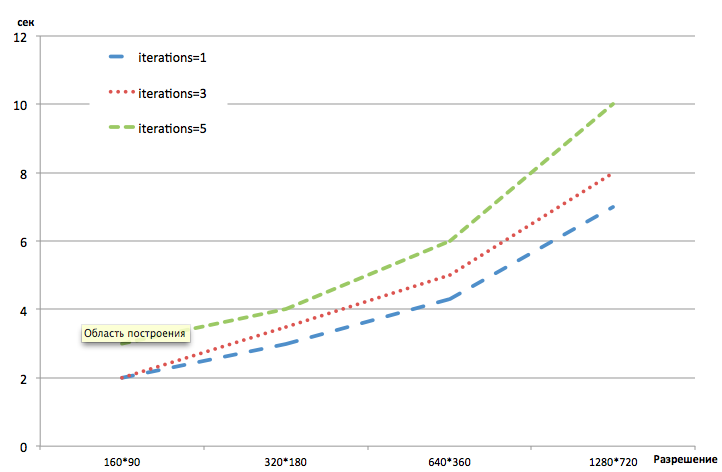
\includegraphics[width=1\linewidth]{pics/3FB_interation.png}} г) \\
\end{minipage}

\begin{center}
	\begin{minipage}[h]{0.47\linewidth}
	\center{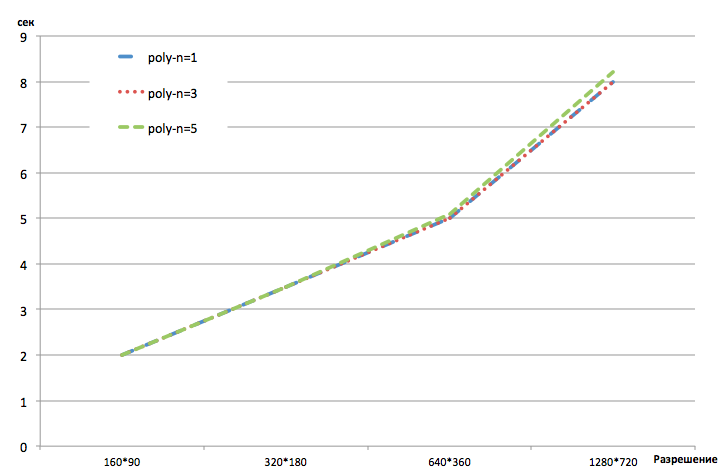
\includegraphics[width=1\linewidth]{pics/3FB_polyn.png}} д) \\
	\end{minipage}
\end{center}
\caption{Влияние значения параметров на время работы алгоритма: а)pyr--scale; б)  levels; в) winsize ; г) interation; д) poly--n}
\label{pic:3FB_params}
\end{figure}

Из графиков видно, что снизить время выполнения можно путем уменьшения уровней в пирамиде, однако такой подход снижает точность вычисления оптического потока. К сожалению, выразить точность вычисления в измеримой величине сложно. Такая же ситуация с числом итераций interation - снижение их числа снижает время выполнения, но качество вычисления потока снижается. 

\paragraph{SimpleFlow}
Согласно документации OpenCV метод SimpleFlow имеет следующие параметры.
\begin{itemize}
\item \textit{prev} – первое изображение.
\item \textit{next} – второе изображение.
\item \textit{flow} – вычисленный оптический поток в виде векторов. 
\item \textit{layers} – число уровней при построении пирамиды. Стандартное значение - 3.
\item \textit{averaging--block--size} – размер окна, по которому происходит поиск пикселей. Стандартное значение - 2. 
\item \textit{max--flow} – максимальный сдвиг для всех уровней пирамиды. Стандартное значение - 4.
\end{itemize}

Так же очевидно, что первые три параметра являются опорными и не подлежат изменению в рамках эксперимента. Влияние последних трех параметров на время вычисления оптического потока методом SimpleFlow показано на рисунке~\ref{pic:3SF_params}
\begin{figure}[!Htb]
\begin{minipage}[h]{0.47\linewidth}
\center{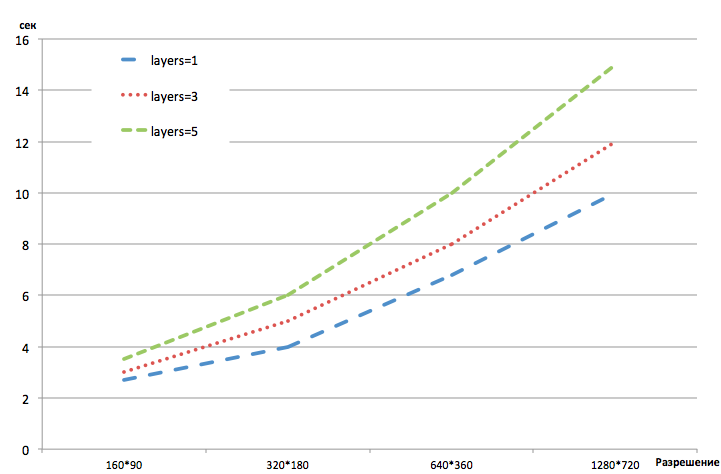
\includegraphics[width=1\linewidth]{pics/3SF_layers.png}} a) \\
\end{minipage}
\hfill
\begin{minipage}[h]{0.47\linewidth}
\center{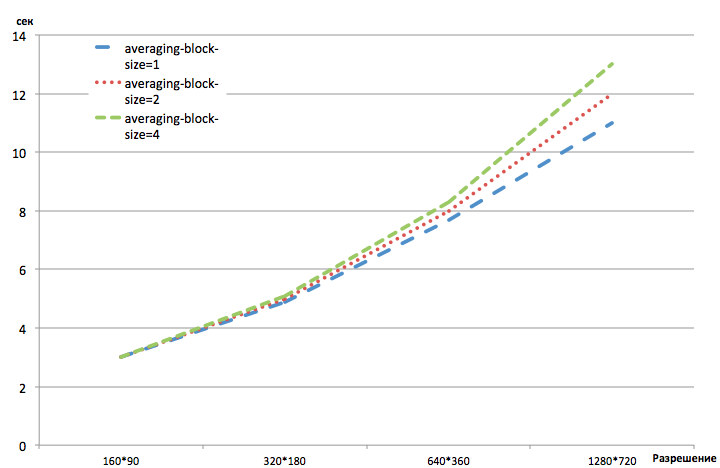
\includegraphics[width=1\linewidth]{pics/3SF_avgBlockSize.png}} б)\\
\end{minipage}
\vfill
\begin{center}
	\begin{minipage}[h]{0.47\linewidth}
	\center{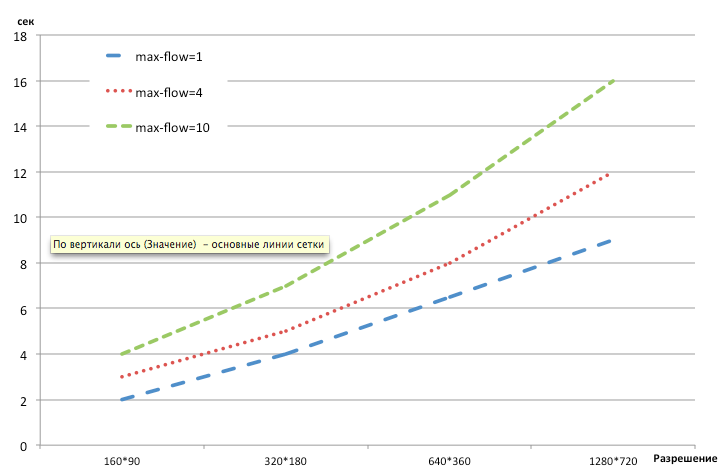
\includegraphics[width=1\linewidth]{pics/3SF_maxflow.png}} в) \\
	\end{minipage}
\end{center}
\caption{Влияние значения параметров на время работы алгоритма: а)layers; б)  averaging--block--size; в) max--flow;}
\label{pic:3SF_params}
\end{figure}

Из графиков видно, что наибольшее влияние оказывает параметр max--flow, но так как он ограничивает значения максимального оптического потока, то для нахождения всех возможных сдвигов в ходе быстрого движения в кадре, этот параметр должен быть близок к  $max (высота кадра, ширина кадра) $. Таким образом, уменьшение данного параметра до 1, снижает время вычисления, но делает работу алгоритма бессмысленной, так как сдвиги более чем на 1 пиксель не будут найдены.  


\subsection{Выводы к исследовательской части}
В ходе проведения экспериментов было установлено следующее:
\begin{itemize}
\item Алгоритм Лукаса-Канаде работает быстрее алгоритмов SimpleFlow и Farneback. Причем разница более заметна при больших разренениях кадра. 
\item Алгоритмы SimpleFlow и Farneback имеют несколько параметров, оказывающих влияние на время их выполнения, однако при уменьшении времени выполнения снижается и качество вычисления результирующего оптического потока. 
\item При необходимости высчитывать оптический поток в реальных условиях, самым приемлемым является алгоритм Лукаса-Канаде, которые показывает наименьшее время выполнения при приемлемом качестве. Такое преимущество возникает из-за вычисления не плотного, а выборочного оптического потока. 
\end{itemize}
\newpage

\section{Экономическая часть}
\subsection{Обоснование сметы  затрат на разработку программного продукта ПАОПО}

Процесс разработки сложного программного продукта сопровождается необходимостью решения многих экономических проблем. Одна из важных экономических проблем – определение стоимости программного продукта (ПП), т.е.  сметной стоимости затрат  на его разработку.

Затраты на разработку программного продукта могут быть представлены в виде сметы затрат, включающей в себя следующие статьи:
\begin{itemize}
	\item расходные материалы;
	\item затраты на оборудование;
	\item затраты на оплату труда;
	\item накладные расходы;
	\item услуги сторонних организаций;
	\item прочие расходы;
\end{itemize}

Расчет затрат на разработку данного программного продукта проводился для уровня цен и окладов на 22.04.2014г.

\subsubsection{Расчет затрат на расходные материалы}

   В статье учитываются суммарные затраты на расходные материалы, приобретаемые для разработки данного программного продукта (ПП), которые указаны в Таблице~\ref{tab:a}.
 
\renewcommand{\arraystretch}{1.4} %% increase table rowspacing   
\begin{table}[!htb]
	\caption{Стоимости расходных материалов и инструментов}\label{tab:a}
    \centering
        \begin{tabular}{|l|l|l|}
        		\hline
        		Наименование & Кол-во & Цена \\
        		\hline
        		Win Home Basic 7 SP1 32-bit Russian & 2 & 2 464 руб \\
        		\hline
        		Visual Studio Professional 2012 & 1 & 13 998 руб\\
        		\hline
        		IntelliJ IDEA 13 & 1 & 7 500 руб\\ 
        		\hline
        		IntelliJ IDEA 13 & 1 & 7 500 руб\\ 
        		\hline
        		\multicolumn{3}{|l|}{канцелярские товары}\\
        		\hline
        		писчая бумага А4 (пачка) & 1 & 140 руб\\
        		\hline
        		ручки, карандаши, ластики &   & 100 руб\\
        		\hline
        		CD – RW диск & 1 & 40 руб\\
        		\hline
        		\multicolumn{3}{|r|}{Итого: 24 242 руб }\\
        		%\hline
        		%\multicolumn{3}{|r|}{24 242 руб}\\
        		\hline
        \end{tabular}
    		
\end{table}

Получаем, что  затраты на расходные материалы составляют 
СМ=24 242 руб.


\subsubsection{Расчет затрат на оборудование}

В статье учитываются суммарные затраты на использование оборудования.
$$ 
C_{эвм}=
\frac{Ц_{эвм} \cdot Т_{эвм}}{Т_{АМР}} =
\frac{12 000 \cdot 3}{5 \cdot 12} = 
600 \; руб
$$
где, 

$C_{эвм}$ — затраты на использование (аренду) ПЭВМ для разработки программного продукта

$Ц_{эвм}$ — покупная цена вычислительной техники: $Ц_{эвм} = 12 \; 000 \; руб$

$Т_{эвм}$ — время использования ПЭВМ для разработки данного программного продукта в месяцах (3 месяца)

$Т_{АМР}$ – срок амортизации вычислительной техники, составляет 5 лет. 

Тогда $Т_{АМР} = 5 \; лет =5 \cdot 12 = 60 \; месяцев $.

Затраты на ремонт вычислительной техники составляют 5\% от  стоимости ее использования и равны:
$$C_{рем} = 0,05 \cdot C_{эвм} = 30 \; руб$$

Получаем, что  затраты на оборудование с учетом его ремонта составляют:
$ С_{ОБ} = С_{ЭВМ} + С_{РЕМ} =  600 + 30 = 630 \; руб$.

\subsection{Определение трудоемкости выполнения проекта}
Трудоемкость разработки проекта по каждому участнику может быть определена как сумма величин трудоемкости выполнения участниками отдельных стадий.

В соответствии с ГОСТ 19.102-94 “Стадии разработки” процесс разработки ПОАПО разбивается на пять стадий: разработка ТЗ, эскизное проектирование, техническое проектирование, рабочее проектирование и внедрение. Этот ГОСТ допускает в технико-обоснованных случаях исключать стадии эскизного и технического проектов, то есть объединять техническое и рабочее проектирование. Трудоемкость каждого этапа указывается в часах и приведена в  Таблице~\ref{tab:b}.

\begin{table}[!htb]
	\caption{Трудоемкость по этапам проектирования}\label{tab:b}
    \centering
        \begin{tabular}{|p{4cm}|p{5.5cm}|l|l|}
        		\hline
        		\multirow{2}{4cm}{Стадия} & \multirow{2}{*}{Этап} & \multicolumn{2}{c|}{Трудоёмкость (часы)} \\
        		\cline{3-4}
            	& & Аналитик & Разработчик \\
            	\hline	
            	\multirow{3}{*}{1. Разработка ТЗ} 
            						& 1.1 Формулировка и уточнение задания. 
            						& 20 & – \\
            	\cline{2-4}	
                					& 1.2. Исследование и анализ ПО. 
            						& 80 & – \\
            	\cline{2-4}	
            	    					& 1.3. Разработка и утверждение ТЗ. 
            						& 40 & – \\
            	\hline	
            	\multirow{3}{4cm}{2. Рабочее
проектирование
} 
            						& 2.1. Техническое проектирование (разработка моделей данных и алгоритмов).
            						& 200 & 20 \\
            	\cline{2-4}	
                					& 2.2. Рабочее проектирование (кодирование и тестирование программных модулей). 
            						& 20 & 160 \\
            	\cline{2-4}	
            	    					& 2.3. Тестовые испытания системы. 
            						& 20 & 100 \\
            	\cline{2-4}	
            	    					& 2.4. Разработка программной документации.
            						& 60 & - \\						
        		\hline
        		3. Внедрение & 3.1. Подготовка проекта к внедрению. & 40 & 20 \\
        		\hline
        		\multicolumn{2}{|l|}{Итого по участникам:} & 480 & 300 \\
        		\hline
        		\multicolumn{2}{|l|}{Итого:} & \multicolumn{2}{c|}{ 780 } \\
        		\hline
        \end{tabular}   		
\end{table}

Для определения трудоемкости разработки проекта по каждому участнику в человеко-днях, используем следующую формулу: 
$$ T_{рд} = Т_{час}/t_{рд},$$
где $Т_{час}$ – время на разработку в часах, $t_{рд}$ – коэффициент, показывающий количество рабочих часов в одном дне. Для дальнейших расчетов примем $t_{рд} = 8\; час$

Для аналитика $T_{рд} = Т_{час}/t_{рд} = 480/8 = 60 \; дней$.

Для разработчика $T_{рд} = Т_{час}/t_{рд} = 300/8 = 38 \; дней$.

Или, суммарно, – 98 рабочих дней.

Для определения времени реализации проекта требуется перевести рабочие дни в календарные дни (КД). Для перевода используется следующая формула:

$$Т_{кд}=\frac{T_{РД} \cdot (1+d) }{g},$$
где $d$ – доля дополнительных работ, порученных другой группе работников попутно с основной работой (от 0,1 до 0,3). В нашем случае проект ведётся самостоятельно, $d = 0$, $g$ – коэффициент перевода (в зависимости от выходных и праздничных дней) – 0,73.

Дня аналитика: $Т_{кд}={T_{РД} \cdot (1+d) }/{g} = 60/0,73 = 83 $ календарных дня.

Для разработчика: $Т_{кд}={T_{РД} \cdot (1+d) }/{g} = 38/0,73 = 52 $ календарных дня.

Или, суммарно, – 135 календарных дней.

\subsection{Расчет затрат на оплату труда}

В данную статью включается заработная плата исполнителей, непосредственно связанных с разработкой программного продукта, с учетом их должностного оклада и времени участия в разработке. 

Основная заработная плата рассчитывается по формуле:
$$ЗП_{осн}=T_{д} \cdot L_{ср.дн.},$$
где $T_{д}$ – трудоемкость, календарные дни, $L_{ср.дн.}$ – среднедневной заработок работника. 

Для определения средней заработной платы аналитика-руководителя небольшого проекта и программиста-разработчика проведен анализ основных ресурсов, предоставляющих сервисы для поиска работы и дающих возможность оценить размер компенсации труда. Такой подход позволяет оценить максимально приближенную к реальности рыночную стоимость труда.

Использованные ресурсы:
\begin{itemize}
	\item портал поиска предложений по трудоустройству HeadHunter. Адрес: www.hh.ru
	\item портал поиска предложений по трудоустройству Job.ru. Адрес: www.job.ru.
\end{itemize}

В результате в качестве средней заработной платы аналитика-руководителя проекта было взято 50 тыс. руб., программиста – 60 тыс. руб.

Тогда среднедневной заработок находится по формуле:

$$L_{ср.дн.}=L_{0}/F,$$ 
где $L_{0}$ – среднемесячная заработная плата, $F$ – среднее количество рабочих дней в месяце. F вычисляется по следующей формуле:

$$ F = \frac{\sum N_{раб}}{n} = \frac{18+19+22}{3} = 19,$$
где $N_{раб}$ – количество рабочих дней в месяце, $n$ – число месяцев.

В данном случае n = 3.

Тогда, для аналитика $L_{ср.дн.}= 50 000 / 19 = 2 631 руб.$ и расходы на основную зарплату составят: $ЗП_{осн} = 2 631 \cdot 60 дней \approx 158 000 руб.$

Тогда, для разработчика  $ L_{ср.дн.}= 60 000 / 19 = 3 157 руб.$ и расходы на основную зарплату составят: $ЗП_{осн} = 3 157 \cdot 38 дней \approx 120 000 руб.$

\textbf{Дополнительная  заработная плата.}

Расходы на дополнительную заработанную плату учитывают все выплаты непосредственно исполнителям за время не проработанное на производстве, но предусмотренное законодательством, в том числе: оплата очередных отпусков, компенсация за недоиспользованный отпуск, и др. Величина этих выплат составляет 20\% от размера основной заработной платы:

$$С_{зпд} = 0,2 \cdot С_{зпо} = 0,2 \cdot 278\;000 = 55\;600 \; руб$$

В результате получаем, что  затраты на  оплату труда составляют:
$$С_{зпи} = С_{зпо} + С_{зпд} = 278\;000 + 55\;600 = 333\;600 руб.$$

\subsubsection{Расчет затрат на  страховые взносы}

В данной статье затрат учитываются отчисления на социальные нужды, производимые в фонды социального страхования, обязательного медицинского страхования и пенсионный фонд. Расчет производится с учетом законов, принятых с 1 января 2012 года (отдельные положения вступают в иные сроки):

Федеральный закон от 24.07.2009  \textnumero 212 ФЗ (ред. от 28.12.2013) <<О страховых взносах в Пенсионный фонд Российской Федерации, Фонд социального страхования Российской Федерации, Федеральный фонд обязательного медицинского страхования и территориальные фонды обязательного медицинского страхования>>;

Федеральный закон от 24.07.2009 \textnumero 213 ФЗ (ред. от 07.05.2013) <<О внесении изменений в отдельные законодательные акты Российской Федерации и признании утратившими силу отдельных законодательных актов (положений законодательных актов) Российской Федерации в связи с принятием Федерального закона <<О страховых взносах в Пенсионный фонд Российской Федерации, Фонд социального страхования Российской Федерации, Федеральный фонд обязательного медицинского страхования и территориальные фонды обязательного медицинского страхования>>.

С 1-го января 2006 года согласно федеральному закону РФ \textnumero 158-ФЗ от 6.12.2005 года величина единого социального налога рассчитывается по формуле:

$$ С_{сн}=К^{сн} \cdot C_{зп},$$
где $К^{сн}$ – коэффициент, учитывающий социальный налог, $C_{зп}$ – заработная плата (руб.)

Плательщиками страховых взносов являются страхователи, определяемые в соответствии с федеральными законами о конкретных видах обязательного социального страхования, к которым относятся:
\begin{enumerate}
\item лица, производящие выплаты и иные вознаграждения физическим лицам: 
\begin{itemize}
\item организации;
\item индивидуальные предприниматели;
\item физические лица, не признаваемые индивидуальными предпринимателями;
\end{itemize}
\item индивидуальные предприниматели, адвокаты, нотариусы, занимающиеся частной практикой, и иные лица, занимающиеся в установленном законодательством Российской Федерации порядке частной практикой (далее - плательщики страховых взносов, не производящие выплаты и иные вознаграждения физическим лицам), если в федеральном законе о конкретном виде обязательного социального страхования не предусмотрено иное.
(в ред. Федерального закона от 03.12.2011 \textnumero 379-ФЗ).
Для страхователей, перечисленных выше, предусмотрены следующие ставки:
\end{enumerate}
\begin{table}[!htb]
    \centering
        \begin{tabular}{|l|l|l|}
        		\hline
        		ПФР & ФСС & ФФОМС \\
        		\hline
        		22\% & 2,9\% & 5,1\% \\
        		\hline
        \end{tabular}   		
\end{table}

Отсюда  $К^{сн} = 0,3$  и таким образом затраты на единый социальный налог составляют: $С_{СН} = 0,3  \cdot 333 \; 600  \; руб = 100 \; 080 \; руб.$

\subsubsection{Расчет затрат на услуги сторонних организаций} 

В статье учитываются затраты на выполнение сторонними организациями работ, непосредственно связанных с разработкой программного продукта.

При разработке данного продукта потребовались услуги сторонних организаций по изготовлению 10-ти плакатов формата A1 и печати на принтере 300 листов РПЗ формата А4.  Стоимость распечатки плакатов  (СПЛ) и листов РПЗ (СЛ) соответственно  рассчитываются  по формулам:
$$С_{ПЛ} =10 \cdot С_{А1} = 10 \cdot 150 = 1500 \; руб,$$
где $С_{А1}$ – стоимость распечатки одного плаката формата A1.   $С_{А1}  = 150 руб.$.
$$С_Л =300 \cdot С_{А4} = 300 \cdot 2 = 600 \; руб.,$$
где $С_{А4}$ – стоимость распечатки одного листа  формата А4. $С_{А4}  = 2 \; руб.$

Получаем, что затраты на услуги сторонних организаций составляют
$С_{ИЗГ}= С_{ПЛ} + С_Л = 2100 \; руб.$

\subsubsection{Расчет затрат на накладные расходы}
В данной статье учитываются затраты на общехозяйственные расходы (это плата за здание, в котором идет разработка, его ремонт, плата за энергоресурсы), непроизводственные расходы и расходы на управление.
Накладные расходы составляют 12,5\% + 25\% требуемого уровня рентабельности.
 
$С_{НР}  =(0,125+0,25) \cdot (С_М + С_{ОБ} + С_{ЗП} + С_{СН} + С_{ИЗГ})$

Таким образом,  затраты на накладные расходы составляют:  
$С_{НР}  = (0,125+0,25) \cdot (18 \; 480+ 630 + 333 \; 600+ 100 \; 080 + 2 \; 100) =170 \; 583,75 руб.$

\subsubsection{Расчет прочих расходов}

Данная статья расходов учитывает налог на имущество и налог на транспортные средства. Налог на имущество в данном случае не платится, так как  все имущество, включаемое в налогооблагаемую базу в соответствии с инструкцией «О порядке исчисления и уплаты в бюджет налога на имущество предприятий», используется на нужды образования, и, следовательно, налогом на имущество не облагается.

Налог на владельцев транспортных средств не платится, в связи с отсутствием транспортных средств. 

\subsubsection{Итог затрат для заказчика}

Итог затрат для заказчика рассчитывается как сумма по всем вышеперечисленным статьям затрат и составляет:

$Ц = 24 \; 242+ 630 + 333 \; 600  + 100 \; 080  + 2100 + 170 \; 583   =  625 \; 473  руб.$

Смета затрат на разработку программного продукта приведена в Таблице~\ref{tab:c}.

\begin{table}[!htb]
	\caption{Стоимости расходных материалов и инструментов}\label{tab:c}
    \centering
        \begin{tabular}{|l|l|l|}
        		\hline
        		\textnumero п/п & Статья затрат & Сумма статьи (руб.) \\
        		\hline
        		1 & Расходные материалы & 24 242 \\
        		\hline
        		2  & Затраты на оборудование & 630 \\
        		\hline
        		3  & Затраты на оплату труда & 333 600 \\
        		\hline
        		4  & Услуги сторонних организаций & 2 100 \\
        		\hline
        		5  &  Накладные расходы & 170 583 \\
        		\hline
        		6 & Прочие расходы & - \\
        		\hline
        		7 & Цена & 631 315 \\
        		\hline
        \end{tabular}   		
\end{table}


\subsection{Основные сметы затрат на тестирование, внедрение и эксплуатацию системы}

Далее рассчитаем затраты на внедрение и эксплуатацию программного продукта ПАОПО.

\subsubsection{Тестирование}
Для тестирования разрабатываемой подсистемы необходимо выполнить следующие пункты:
\begin{itemize}
\item сопрячь ПАОПО с видеокамерой;
\item сопрячь ПАОПО с инерциальными измерительными приборами;
\item провести тестирование ПАОПО, фиксируя перемещения с помощью GPS-трекера;
\item наложить полученные с помощью ПАОПО данных на данные, полученные с помощью GPS-трекера.
\end{itemize}

Таким образом необходимо закупить следующее оборудование:
\begin{itemize}
\item видеокамера с разрешением 720*1080;
\item трехосевой гироскоп;
\item трехосевой акселерометр;
\item GPS-трекер;
\end{itemize}

Данное оборудование установлено во всех современных смартфонах, работающих под управлением ОС Android, стоимость которых в настоящее время составляет 6 000 рублей и более. Например, телефон HTC Sensation, удовлетворяющий всем требованиям стоит 6200 рублей. 

Для проведения сопряжения полученных данных с ПАОПО необходимо написать простое приложение, фиксирующее все данные в нужном формате для анализа разрабатываемой подсистемы, разработка которого займет до двух рабочих дней Android-разработчка. 

Согласно приведенным выше данным стоимость одного дня разработчика составляет 3 157 рублей. С учетом дополнительных расходов и отчислений в страховые фонды затраты на создание приложения составят:

$$31571,2 \cdot 1,3 \cdot 2=9 \; 849 \; руб$$

Таким образом затраты на тестирование составят 16 149 рублей.

\subsubsection{Внедрение и эксплуатация}

В рамках создания ПАОПО не предусмотрены внедрение и эксплуатация, так как подсистема может работать лишь в составе другой автономной системы. 

ПАОПО является кроссплатформенной, что позволяет в кратчайшие сроки интегрировать ее в любую другую систему. При этом разработчику этой системы необходимо согласовать вход и выход ПАОПО, корректно предоставляя и получая данные в/из подсистемы. Суммарные затраты на проведение интеграции могут занимать до двух рабочих дней разработчика. Согласно приведенным выше данным стоимость этой работы составит не более 6 314 рублей. 

Однако данные затраты не относятся к стоимости создания ПАОПО, а перекладываются на ее потребителей. 

\subsection{Итого. Расходы на разработку  и тестирование.}
\begin{table}[tb!h]
	\caption{Итого. Расходы на внедрение и эксплуатацию системы.}
    \centering
        \begin{tabular}{|l|l|l|}
        		\hline
        		\textnumero п/п & Статья затрат & Сумма статьи (руб.) \\
        		\hline
        		1 & Стоимость программного продукта ПОАПО & 631 315 \\
        		\hline
        		\multicolumn{3}{|r|}{\textbf{Итого: 647 646} }\\
        		\hline
        \end{tabular}   		
\end{table}
\newpage

\section{Промышленная экология и безопасность}
\subsection{Анализ опасных и вредных факторов, возникающих при работе на ПЭВМ}
Для обеспечения комфортных условий труда сотрудника организации, рабочее место которого включает ПЭВМ, необходимо выполнение следующие требования\cite{SanPinGigiena}:
\begin{enumerate}
\item требования к ПЭВМ, установленные в СанПин 2.2.2/2.4.1340-03 <<Гигиенические требования к персональным электронно-вычислительным машинам и организации работы>>;
\item требования к помещениям для работы с ПЭВМ;
\item требования к организации и оборудованию рабочих мест с ПЭВМ;
\item требования к микроклимату помещения, установленные в  СанПиН \\2.2.4.548-96 <<Гигиенические требования к микроклимату производственных помещений>>;
\item требования к освещению на рабочих местах, оборудованных ПЭВМ
\item требования к уровням шума и вибрации на рабочих местах, оборудованных ПЭВМ;
\item требования к режиму труда и отдыха.
\end{enumerate}

\subsubsection{Помещение для работы с ПЭВМ}

Ниже приведены основные требования, предъявляемые к помещениям, предназначенным для работы сотрудников с ПЭВМ.

Помещения для эксплуатации ПЭВМ должны иметь естественное и искусственное освещение. Эксплуатация ПЭВМ в помещениях без естественного освещения допускается только при соответствующем обосновании и наличии положительного санитарно-эпидемиологического заключения, выданного в установленном порядке.

Окна в помещениях, где эксплуатируется вычислительная техника, преимущественно должны быть ориентированы на север и северо-восток. Оконные проемы должны быть оборудованы регулируемыми устройствами типа: жалюзи, занавесей, внешних козырьков и др.

Для внутренней отделки интерьера помещений, где расположены ПЭВМ, должны использоваться диффузно-отражающие материалы с коэффициентом отражения для потолка – 0,7 - 0,8; для стен – 0,5 - 0,6; для пола – 0,3 - 0,5.

Полимерные материалы используются для внутренней отделки интерьера помещений с ПЭВМ при наличии санитарно-эпидемиологического заключения.

Помещения, где размещаются рабочие места с ПЭВМ, должны быть оборудованы защитным заземлением (занулением) в соответствии с техническими требованиями по эксплуатации.

\subsubsection{Рабочее место оператора и положение за рабочим местом}
\paragraph{Общие требования}

При размещении рабочих мест с ПЭВМ расстояние между рабочими столами с видеомониторами (в направлении тыла поверхности одного видеомонитора и экрана другого видеомонитора), должно быть не менее 2,0 м, а расстояние между боковыми поверхностями видеомониторов не менее 1,2 м.

Рабочие места с ПЭВМ в помещениях с источниками вредных производственных факторов должны размещаться в изолированных кабинах с организованным воздухообменом. 

Рабочие места с ПЭВМ при выполнении творческой работы, требующей значительного умственного напряжения или высокой концентрации внимания, рекомендуется изолировать друг от друга перегородками 1,5 – 2,0 м.

Экран видеомонитора должен находиться от глаз пользователя на расстоянии 600-700 мм, но не ближе 500 мм с учетом размеров алфавитно-цифровых знаков и символов.

Конструкция рабочего стола должна обеспечивать оптимальное размещение на рабочей поверхности используемого оборудования с учетом его количества и конструктивных особенностей, характера выполняемой работы.

При этом допускается использование рабочих столов различных конструкций, отвечающих современным требованиям эргономики. Поверхность рабочего стола должна иметь коэффициент отражения 0,5 – 0,7.

Конструкция рабочего стула (кресла) должна обеспечивать поддержание рациональной рабочей позы при работе на ПЭВМ, позволять изменять позу с целью снижения статического напряжения мышц шейно-плечевой области и спины для предупреждения развития утомления. Тип рабочего стула (кресла) следует выбирать с учетом роста пользователя, характера и продолжительности работы с ПЭВМ.

Рабочий стул (кресло) должен быть подъемно-поворотным, регулируемым по высоте и углам наклона сиденья и спинки, а также расстоянию спинки от переднего края сиденья, при этом регулировка каждого параметра должна быть независимой, легко осуществляемой и иметь надежную фиксацию.

Поверхность сиденья, спинки и других элементов стула (кресла) должна быть полумягкой, с нескользящим, слабо электризующимся и воздухопроницаемым покрытием, обеспечивающим легкую очистку от загрязнений.

\paragraph{Требования к значениям параметров рабочего места}

Значения параметров рабочего стола приведены в таблице~\ref{bzd:workplace}.

\begin{table}[!htb]
	\caption{Значения параметров рабочего стола}\label{bzd:workplace}
    \centering
    \begin{tabular}{|p{10cm}|p{6cm}|}
        \hline 
        \textbf{Параметры рабочего стола} & \textbf{Значения, мм} \\ 
        \hline 
        Высота рабочей поверхности & регулировка 680-800,
или фиксировано 725 \\ 
        \hline 
        Ширина рабочей поверхности & 1200 \\ 
        \hline 
        Глубина рабочей поверхности & 800 \\ 
        \hline 
        Высота пространства для ног & 750 \\ 
        \hline 
        Ширина пространства для ног & 900 \\ 
        \hline 
        Глубина пространства для ног на уровне колен & 900 \\ 
        \hline 
        Глубина пространства для ног на уровне вытянутых ног & 900 \\ 
        \hline 
        \end{tabular}     
    		
\end{table}

Конструкция рабочего стула (кресла) должна обеспечивать поддержание рациональной рабочей позы при работе на ПЭВМ, позволять изменять позу с целью снижения статического напряжения мышц шейно-плечевой области и спины для предупреждения развития утомления. Тип рабочего стула (кресла) следует выбирать с учетом роста пользователя, характера и продолжительности работы с ПЭВМ.

Рабочий стул (кресло) должен быть подъемно-поворотным, регулируемым по высоте и углам наклона сиденья и спинки, а также расстоянию спинки от переднего края сиденья, при этом регулировка каждого параметра должна быть независимой, легко осуществляемой и иметь надежную фиксацию.

Конструкция рабочего стула должна обеспечивать поверхность сиденья с закругленным передним краем, а также соответствие значений параметров приведённым в таблице~\ref{bzd:workchair}.

\begin{table}[!htb]
	\caption{Значения параметров рабочего стула (кресла)}\label{bzd:workchair}
    \centering
    \begin{tabular}{|p{10cm}|p{6cm}|}
        \hline 
        \textbf{Параметры рабочего стыла (кресла)} & \textbf{Значения} \\ 
        \hline 
        Ширина и глубина поверхности сиденья & не менее 400 мм \\ 
        \hline 
        Высота поверхности сиденья & 400 – 550 мм \\ 
        \hline 
        Угол наклона поверхности сиденья вперед (назад) & до 15 (5) градусов \\ 
        \hline 
        Высота опорной поверхности спинки & 280 – 320 мм \\ 
        \hline 
        Ширина опорной поверхности спинки & не менее 380 мм \\ 
        \hline 
        Радиус кривизны горизонтальной плоскости спинки & 400 мм \\ 
        \hline 
        Угол наклона спинки в вертикальной плоскости & $\pm$ 30 градусов \\ 
        \hline 
        Расстояние спинки от переднего края сиденья & 260 – 400 мм \\ 
        \hline 
        Длина подлокотников & не менее 250 мм \\ 
        \hline 
        Ширина подлокотников & 50 – 70 мм \\ 
        \hline 
        Высота подлокотников над сиденьем & 200 – 260 мм \\ 
        \hline 
        Внутреннее расстояние между подлокотниками & 350 – 500 мм \\ 
        \hline 
        \end{tabular}     
    		
\end{table}

Рабочее место пользователя ПЭВМ следует оборудовать подставкой для ног, имеющей ширину не менее 300 мм, глубину не менее 400 мм, регулировку по высоте в пределах до 150 мм и по углу наклона опорной поверхности подставки до 20 градусов. Поверхность подставки должна быть рифленой и иметь по переднему краю бортик высотой 10 мм.

Клавиатуру следует располагать на поверхности стола на расстоянии 100 – 300 мм от края, обращенного к пользователю или на специальной, регулируемой по высоте рабочей поверхности, отделенной от основной столешницы.

\paragraph{Микроклимат}
Оптимальные микроклиматические условия установлены по критериям оптимального теплового и функционального состояния человека. Они обеспечивают общее и локальное ощущение теплового комфорта в течение 8-часовой рабочей смены при минимальном напряжении механизмов терморегуляции, не вызывают отклонений в состоянии здоровья, создают предпосылки для высокого уровня работоспособности и являются предпочтительными на рабочих местах.
 
В помещениях, в которых работа с использованием ПЭВМ является основной и связана с нервно-эмоциональным напряжением, должны обеспечиваться оптимальные параметры микроклимата. 

В санитарных нормах СанПиН 2.2.2/2.4.1340-03 установлены величины параметров микроклимата, создающие комфортные условия\cite{SanPinAeroIon}. Эти нормы устанавливаются в зависимости от времени года, характера трудового процесса и характера производственного помещения (значительные или незначительные тепловыделения). В данном дипломном проекте рассматриваются условия труда пользователей ПЭВМ, которые относятся к категории Iа, (интенсивность энергозатрат до 120 ккал/ч (до 139 Вт), работа, производимая сидя и сопровождающиеся незначительным физическим напряжением). Величины микроклиматических параметров приведены в таблице~\ref{bzd:microclimat}.

\begin{table}[!htb]
	\caption{Оптимальные параметры микроклимата в помещении}\label{bzd:microclimat}
    \centering
	\begin{tabular}{|p{2cm}|p{2,5cm}|p{2,5cm}|p{3cm}|p{3cm}|p{2,7cm}|}
	\hline 
	Период года & 
	Категория работ по уровню & 
	Темпера тура воздуха,$^{\circ}С$ &
	Температура поверхно стей,$^{\circ}С$ &
	Относи\par тельная влажность воздуха, \% & 
	Скорость движения воздуха, м/с \\ 
	\hline 
	Холод-\par ный & Ia (до 139) & 22-24 & 21-25 & 60-40 & 0,1 \\ 
	\hline 
	Теплый & Ia (до 139) & 23-25 & 22-26 & 60-40 & 0,1\\ 
	\hline 
	\end{tabular} 
    		
\end{table}

Перепады температуры воздуха по высоте и по горизонтали, а также изменения температуры воздуха в течение смены при обеспечении оптимальных величин микроклимата на рабочих местах не должны превышать 2 $^{\circ}С$.

\paragraph{Аэроионный состав воздуха}

В связи с тем, что разработка данного дипломного проекта производилась в помещении, в отделке и (или) меблировке которых используются синтетические материалы или покрытия, способные накапливать электростатический заряд; а так же - в которых эксплуатируется оборудование, способное создавать электростатические поля, включая видеодисплейные терминалы и прочие виды оргтехники, то необходимо учесть действующие <<Гигиенические требования к аэроионному составу воздуха производственных и общественных помещений>> (СанПиН 2.2.4.1294-03), а именно:

\begin{enumerate}
\item Нормируемые показатели аэроионного состава воздуха
	\begin{enumerate}
	\item Аэроионный состав воздуха устанавливается в зависимости от процессов ионизации и деионизации.
	\item Нормируемыми показателями аэроионного состава воздуха производственных и общественных помещений являются:
		\begin{itemize}
			\item концентрации аэроионов (минимально допустимая и максимально допустимая) обеих полярностей р+. р-, определяемые как количество аэроионов в одном кубическом сантиметре воздуха (ион/см\textsuperscript{3});
			\item коэффициент униполярности Y (минимально допустимый и максимально допустимый) определяемый как отношение концентрации аэроионов положительной полярности к концентрации аэроионов отрицательной полярности.
		\end{itemize}
		\item Минимально и максимально допустимые значения нормируемых показателей определяют диапазоны концентраций аэроионов обеих полярностей и коэффициента униполярности, отклонения от которых могут привести к неблагоприятным последствиям для здоровья человека.
		\item Значения нормируемых показателей концентраций аэроионов и коэффициента униполярности приведены в таблице~\ref{bzd:aeroion}.

\begin{table}[!htb]
			\caption{Нормируемые показатели аэроионов и коэффициенты униполярности}\label{bzd:aeroion}
		    \centering
			\begin{tabular}{|p{4cm}|p{3,5cm}|p{3,5cm}|p{3,5cm}|}
			\hline 
			Нормируемые показатели & 
			Концентрация n+ (ион/см\textsuperscript{3}) & 
			Концентрация n-(ион/см\textsuperscript{3}) & 
			Коэффициент униполярности Y\\ 
			\hline 
			Минимально допустимые & n+ $\geq$ 400 &  n- $\geq$ 400 &  0,4 $\leq$ Y $\leq$ 1,0\\ 
			\hline 
			Максимально допустимые & n+ $<$ 50000 & n- $<$ 50000 & ~\ \\ 
			\hline 
			\end{tabular} 
		    		
		\end{table}
		
		\item В зонах дыхания персонала на рабочих местах, где имеются источники электростатических полей (видеодисплейные терминалы или другие виды оргтехники) допускается отсутствие аэроионов положительной полярности.
		\item Степени вредности отклонений от означенных диапазонов концентрации аэроионов и коэффициента униполярности определяются в соответствии с классификацией условий труда по аэроионному составу воздуха.
		\item В лечебных целях могут применяться другие показатели аэроионного состава воздуха если это предусмотрено утвержденными в установленном порядке методиками лечения или применения аэроионизаторов.
	\end{enumerate}
\item Требования к проведению контроля аэроионного состава воздуха
	\begin{enumerate}
	\item Контроль аэроионного состава воздуха осуществляется в следующих случаях: 
		\begin{itemize}
		\item в порядке планового контроля не реже одного раза в год;
		\item при аттестации рабочих мест;
		\item при вводе в эксплуатацию оборудования либо материалов, способных создавать или накапливать электростатический заряд \\(включая видеодисплейные терминалы и прочие виды оргтехники);
		\item при оснащении рабочих мест аэроионизаторами или деионизаторами.
		\end{itemize}
	\item Проведение контроля аэроионного состава воздуха помещений следует осуществлять непосредственно на рабочих местах в зонах дыхания персонала и в соответствии с утвержденными в установленном порядке методиками контроля.
	\end{enumerate}
\item Требования к способам и средствам нормализации аэроионного состава воздуха
	\begin{enumerate}
	\item Если в результате контроля аэроионного состава воздуха выявляется его несоответствие нормированным показателям, рекомендуется осуществление его нормализации.
	\item Осуществление нормализации аэроионного состава воздуха рекомендуется производить на протяжении всего времени пребывания человека на рабочем месте.
	\item Для нормализации аэроионного состава воздуха следует применять соответствующие, прошедшие санитарно-эпидемиологическую оценку и имеющие действующее санитарно-эпидемиологическое заключение аэроионизаторы или деионизаторы предназначенные для использования в санитарно-гигиенических целях.
	\item Санитарно-эпидемиологическая оценка и эксплуатация аэроионизаторов и деионизаторов осуществляется в установленном порядке.

	\end{enumerate}
\end{enumerate}

\paragraph{Шум и вибрация}

На рабочем месте пользователя ПЭВМ источниками шума, как правило, разговаривающие люди, внешний шум, компьютер, принтер, вентиляционное оборудование. Основными источниками внешнего шума являются транспортные потоки на улицах и дорогах.

Нормируемыми параметрами постоянного шума являются уровни звукового давления L, дБ, в октавных полосах частот со среднегеометрическими частотами 31,5; 63; 125; 250; 500; 1000; 2000; 4000 и 8000 Гц. Для ориентировочных расчетов допускается использование уровней звука LА, дБА.

Допустимые уровни звукового давления, уровня звука и эквивалентные уровни звука на рабочих местах должны соответствовать требованиям СанПиН 2.2.2/2.4.1340-03.

Показатели нормируемых уровней шума для помещений офисов, рабочих помещений и кабинетов административных зданий (помещения, где могут располагаться рабочие места сотрудников – разработчиков и эксплуататоров проектируемой системы) приведены в таблице .

Основным из механических факторов производственной среды является вибрация. Она не только вредно действуют на организм, но и мешают человеку выполнять как мыслительные, так и двигатель¬ные операции. 

\begin{table}[!htb]
	\caption{Параметры производственного шума}\label{bzd:noize}
    \centering
	\begin{tabular}{|p{1cm}|p{1cm}|p{1cm}|p{1cm}|p{1cm}|p{1cm}|p{1cm}|p{1cm}|p{1cm}|p{2cm}|}
	\hline 
	\multicolumn{9}{|p{12cm}|}{Уровни звукового давления в октавных полосах со среднегеометрическими частотами} & Уровни звука в дБА \\ 
	\hline 
	31,5 Гц & 63 Гц & 125 Гц & 250 Гц & 500 Гц & 1000 Гц & 2000 Гц & 4000 Гц & 8000 Гц & ~\ \\ 
	\hline 
	86 дБ & 71 дБ & 61 дБ & 54 дБ & 49 дБ & 45 дБ & 42 дБ & 40 дБ & 38 дБ & 50 \\ 
	\hline 
	\end{tabular} 
    		
\end{table}

Шум считают в пределах нормы, когда он как по эквивалентному, так и по максимальному уровню не превышает установленные нормативные значения.
Допустимые уровни шума от внешних источников в помещениях установлены при условии обеспечения нормативного воздухообмена, т.е при отсутствии принудительной системы вентиляции или кондиционирования воздуха, должны выполняться при условии открытых форточек или иных устройств, обеспечивающих приток воздуха.

Защита от шума строительно-акустическими методами должна обеспечиваться:
\begin{itemize}
\item рациональным архитектурно-планировочным решением здания;
\item применением ограждающих конструкций, обеспечивающих нормативную звукоизоляцию;
\item применением звукопоглощающих облицовок в помещении здания;
\item применением глушителей шума в системах принудительной вентиляции и кондиционирования воздуха;
\item виброизоляцией инженерного и санитарно-технического оборудования зданий.
\end{itemize}

\subsubsection{Освещение}
\paragraph{Общие требования}

Ниже приведены основные требования, предъявляемые к освещению помещений, предназначенных для работы сотрудников с ПЭВМ.

Рабочие столы следует размещать таким образом, чтобы видеодисплейные терминалы были ориентированы боковой стороной к световым проемам, чтобы естественный свет падал преимущественно слева.

Искусственное освещение в помещениях для эксплуатации ПЭВМ должно осуществляться системой общего равномерного освещения. В производственных помещениях, в случаях основной работы с документами, можно применять системы комбинированного освещения (к общему освещению дополнительно устанавливаются светильники местного освещения, предназначенные для освещения зоны расположения документов).

Освещенность на поверхности стола в зоне размещения рабочего документа должна быть 300 – 500 лк. Освещение не должно создавать бликов на поверхности экрана. Освещенность поверхности экрана не должна быть более 300 лк.

Следует ограничивать прямую блесткость от источников освещения, при этом яркость светящихся поверхностей (окна, светильники и др.), находящихся в поле зрения, должна быть не более 200 кд/м\textsuperscript{2}.

Следует ограничивать отраженную блесткость на рабочих поверхностях (экран, стол, клавиатура и др.) за чет правильного выбора типов светильников и расположения рабочих мест по отношению к источникам естественного и искусственного освещения, при этом яркость бликов на экране ПЭВМ не должна превышать 40 кд/м\textsuperscript{2} и яркость потолка не должна превышать 200 кд/м\textsuperscript{2}.

Яркость светильников общего освещения в зоне углов излучения от 50 до 90 градусов с вертикалью в продольной и поперечной плоскостях должна составлять не более 200 кд/м\textsuperscript{2}, защитный угол светильников должен быть не менее 40 градусов.

 Светильники местного освещения должны иметь не просвечивающий отражатель с защитным углом не менее 40 градусов.
 
 Следует ограничивать неравномерность распределения яркости в поле зрения пользователя ПЭВМ, при этом соотношение яркости между рабочими поверхностями не должно превышать 3:1 – 5:1, а между рабочими поверхностями и поверхностями стен и оборудования 10:1.

В качестве источников света при искусственном освещении следует применять преимущественно люминесцентные лампы типа ЛБ. При устройстве отраженного освещения в производственных и административно-\\общественных помещениях допускается применение металлогалогенных ламп. В светильниках местного освещения допускается применение ламп накаливания, в том числе галогенные.

Для освещения помещений с ПЭВМ следует применять светильники с зеркальными параболическими решетками, укомплектованными электронными пуско-\\регулирующими аппаратами. Допускается использование многоламповых светильников с электромагнитными пуско-регулирующими аппаратами, состоящими из равного числа опережающих и отстающих ветвей.

Применение светильников без рассеивателей и экранирующих решеток не допускается. При выполнениии работы использовались лампы с экранирующими решетками.

Общее освещение при использовании люминесцентных светильников следует выполнять в виде сплошных или прерывистых линий светильников, расположенных сбоку от рабочих мест, параллельно линии зрения пользователя при рядном расположении видеодисплейных терминалов. 

Коэффициент запаса (Кз) для осветительных установок общего освещения должен приниматься равным 1,4.

Коэффициент пульсации не должен превышать 5\%.

Для обеспечения нормируемых значений освещенности в помещениях для использования ПЭВМ проводится чистка стекол оконных рам и светильников не реже двух раз в год и своевременную замену перегоревших ламп.

\subsubsection{Расчёт освещения}
\paragraph{Искусственное освещение}

Так как минимальным объектом различения при работе с ПЭВМ является пиксель, размер которого составляет 0.28мм, то выполняемый вид работ считаем зрительной работой очень высокой точности\cite{SP52}. 

Нормы для искусственного освещения приведены в таблице~\ref{bzd:svet}.

\begin{table}[!htb]
	\caption{Нормы для искусственного освещения}\label{bzd:svet}
    \centering
	\begin{tabular}{|p{3cm}|p{2,5cm}|p{2cm}|p{2cm}|p{3cm}|p{2cm}|}
	\hline 
	\multirow{2}{3cm}{~\ Характеристика зрительной работы} &
	\multirow{2}{2,5cm}{Размер объекта различения, мм} & 
	\multirow{2}{2cm}{Контраст объекта с фоном} &
	\multirow{2}{2cm}{Фон} &
	\multicolumn{2}{p{5cm}|}{Освещенность, лк}\\ 
	\cline{5-6} 
	 &  &  &  & ~\ Комбинированное освещение &  Общее освещение \\ 
	\hline 
	\multirow{4}{3cm}{Очень высокой точности} &
	\multirow{4}{2,5cm}{0,15 - 0,30} & 
	малый & темный & 4000 & - \\
	\cline{3-6} 
	& & малый & средний & 3000 & 750 \\
	& & средний & темный & 2500 & 600 \\
	\cline{3-6} 
	& & малый & светлый & 2000 & 500 \\
	& & средний & средний & 1500 & 400 \\
	& & большой & темный &  &  \\
	\cline{3-6} 
	& & средний & светлый & 1000 & 300 \\
	& & большой & светлый & 750 & 200 \\
	& & большой & средний &  &  \\
	\hline
	\end{tabular} 
    		
\end{table}

При работе оператора разрабатываемой подсистемы предполагается работа при среднем контрасте и светлом фоне. Таким образом, нормированная минимально-допустимая освещенность при общем освещении составляет 300 лк. 

Основным методом расчета общего равномерного освещения при горизонтальной рабочей поверхности является метод светового потока (коэффициента использования). Необходимый световой поток Фл (лм) от одной лампы накаливания или группы ламп светильника при люминесцентных лампах рассчитывают по формуле \ref{bzd:svetpotok}.

\begin{equation}\label{bzd:svetpotok}
Ф_{осв}=\frac{E_н \cdot S \cdot z \cdot k}{N_c \cdot \eta},
\end{equation}

где $E_н$ – нормированная минимально-допустимая освещенность (лк), которая определяется нормативом (см. таблицу~\ref{bzd:svet}); $S$ — площадь освещаемого помещения (м\textsuperscript{2}); $z$ — коэффициент неравномерности освещения, который зависит от типа ламп (для ламп накаливания и дуговых ртутных ламп — 1,15, для люминесцент¬ных ламп — 1,1); k — коэффициент запаса, соласно \cite{metodaBZD} равен 1,4; $N_c$ — число светильников в помещении; $\eta$ — коэффициент использования светового потока ламп, учитывающий долю общего светового потока, приходящуюся на расчетную плоскость, и зависящий от типа светильника, коэффициента отражения потолка $\rho_п$ и стен $\rho_с$, высоты подвеса светильников, размеров помещения, определяемых индексом i помещения. Индекс помещения определяется по формуле~\ref{bzd:indexroom}

\begin{equation}\label{bzd:indexroom}
i=\frac{A \cdot B }{H_c \cdot (A + B)},
\end{equation}

где $A$ и $В$ — длина и ширина помещения, м; $Н_с$ — высота подвеса светильников над рабочей поверхностью.

Коэффициент использования светового потока ламп опре¬деляют по таблицам, приводимым в СНиП 23—05—95 в зависи¬мости от типа светильника, $\rho_п$, $\rho_с$ и индекса $i$.
По полученному в результате расчета по формуле~\ref{bzd:svetpotok} световому потоку по ГОСТ 2239-79* и ГОСТ 6825-91 выбирают ближайшую стандартную лампу и определяют ее необходимую мощность. Умножив электрическую мощность лампы на количество светильников Nc, можно определить электрическую мощность всего освещения помещения.

Расчет освещения от светильников с люминесцентными лам¬пами целесообразно выполнять, предварительно задавшись типом, электрической мощностью и величиной светового потока ламп. С использованием этих данных необходимое число светильников определяют по формуле~\ref{bzd:numbersvet}.
 
\begin{equation}\label{bzd:numbersvet}
N_c =\frac{E_н \cdot S \cdot z \cdot k}{Ф_{осв} \cdot N_p \cdot \eta},
\end{equation}

Проведем расчет и определим тип и мощность используемых ламп для помещения со следующими параметрами:
\begin{itemize}
\item Ширина $a = 6 м$;
\item Длина	$b = 4 м$;
\item Высота потолков $h = 4 м$;
\item Высота стола $h_c = 0,8 м$;
\item Высота подвеса	$h_р = h – h_c = 3,2 м$.

\end{itemize}

Этапы расчета:
\begin{enumerate}
\item Вычислим индекс помещения:

$$
i=\frac{6 \cdot 4 }{3,2 \cdot (4 + 6)} = 0,75,
$$

\item Число светильников $N$ определим исходя из того, что будет установлено 3 ряда светильников по одному светильнику в ряду:

$$ N = 3 \cdot 2 = 6 шт.$$ 

\item Определим коэффициент использования светового потока по таблицам, приводимым в СНиП 23-05-95, как:
$$ \eta = 0,4 $$
	\begin{itemize}
		\item коэффициента отражения потолка $\rho_п = 70$\%;
		\item коэффициента отражения стен $\rho_с = 50$\%;
	\end{itemize}
	
\item Определим общий необходимый световой поток при условиях:
\begin{itemize}
		\item Коэффициент неравномерности освещения для люминесцентных ламп $z = 1,1$;
		\item Нормированная минимально-допустимая освещенность для общего освещения равна $E_Н = 300 лк$;
		\item Площадь помещения $S=a*b=4*5=20 м^2$;
		\item Коэффициент запаса согласно рекомендуемым в нормативах СанПиН 2.2.2/2.4.1340-03 – $K_З = 1,4$;
	\end{itemize}
	
	$$ Ф_{осв}=\frac{300 \cdot 20 \cdot 1,1 \cdot 1,4}{ 0,4 } = 23 \; 100  \; лк$$
	\item Определим световой поток, приходящийся на один светильник:
	  $$ Ф_{св}= Ф_{осв}/N = {23 \; 100}/3 = 7 \; 700 \; лк $$
	 
	\item Определим световой поток, приходящийся на одну лампу (в применяемых светильниках используется две лампы):
	$$ Ф_л = Ф_{св}/2 = 3\;850 \; лк$$
	 \item Определим тип лампы по таблице:
	 
	   % Table generated by Excel2LaTeX from sheet 'Лист1'
  \begin{table}[!htbp]
    \centering
    \caption{Световой поток наиболее распространенных люминесцентных ламп напряжением 220 В}
      \begin{tabular}{|c|c|c|c|c|c|c|}
      \hline
      \multirow{2}[4]{*}{\textbf{Тип лампы}} & \multicolumn{6}{c|}{\textbf{Световой поток, лм, при мощности, Вт}} \\
\cline{2-7}         & \textbf{15} & \textbf{20} & \textbf{30} & \textbf{40} & \textbf{65} & \textbf{80} \\
      \hline
      ЛДЦ & 500 & 820 & 1450 & 2100 & 3050 & 3560 \\
      \hline
      ЛД & 540 & 920 & 1640 & 2340 & 3575 & 4070 \\
      \hline
      ЛХБ & 675 & 935 & 1720 & 2600 & 3820 & 4440 \\
      \hline
      ЛБ & 760 & 1180 & 2100 & 3000 & 4550 & 5220 \\
      \hline
      \end{tabular}
  \end{table}%


Для значения светового потока $Ф_Л = 3850 \;лм$ подходит два типа ламп:

\begin{itemize}
\item ЛД, 80 Вт, 4070 лм;
\item ЛБ, 65 Вт, 4550 лм.
\end{itemize}

С точки зрения минимизации расхода электроэнергии, выберем второй вариант, т.к. он более экономичный. Суммарный выигрыш в мощности ламп на указанное помещение составит:

$$ \triangle = (80 - 65) \cdot 3 \cdot 2 = 120 \; Вт$$
Сравнение теоретических и практических результатов представлено в таблоице~\ref{bzd:srav}.

 \begin{table}[htbp]
    \centering
    \caption{Сравнение теоретических и практических результатов}\label{bzd:srav}%
      \begin{tabular}{|p{4cm}|p{5cm}|p{5cm}|}
      \hline
       & \textbf{Теоретические (расчетные) значения} & \textbf{Практические значения} \\
      \hline
      Световой поток от одной лампы & 3850 лм & 4550 лм \\
      \hline
      Количество ламп & 12 & 12 \\
      \hline
      Световой поток от всех ламп & 23 100 лм & 27 300 лм \\
      \hline
      \end{tabular}%
    
  \end{table}% 
  Приведенный расчет показал, что практическое значение светового потока больше теоретического на 4200 лм (15\%).
\end{enumerate}
 
  \textbf{Вывод}
  
  В результате проведенных расчетов для рассматриваемого помещения определено:
  \begin{itemize}
  \item Общее количество светильников – 3 штук;
  \item Общее количество ламп – 6 штук (т.к. в каждом светильнике по две лампы);
  \item 	Тип лампы – ЛБ;
  \item Мощность лампы – 65 Вт;
  \item Общий световой поток искусственного освещения – 27 300 лм.
  \end{itemize}

\paragraph{Схема расположения светильников в помещении операторов ПЭВМ}

Светильник скомпонован из двух ламп. Светильники расположены в три ряда по одному светильнику в каждом ряду. Тип используемых ламп – ЛБ–65 (люминесцентная лампа дневного света, мощность 65 Вт).

Схема расположения светильников в помещении изображена на рис.~\ref{pic:room}
\begin{figure}[!htb]
\center{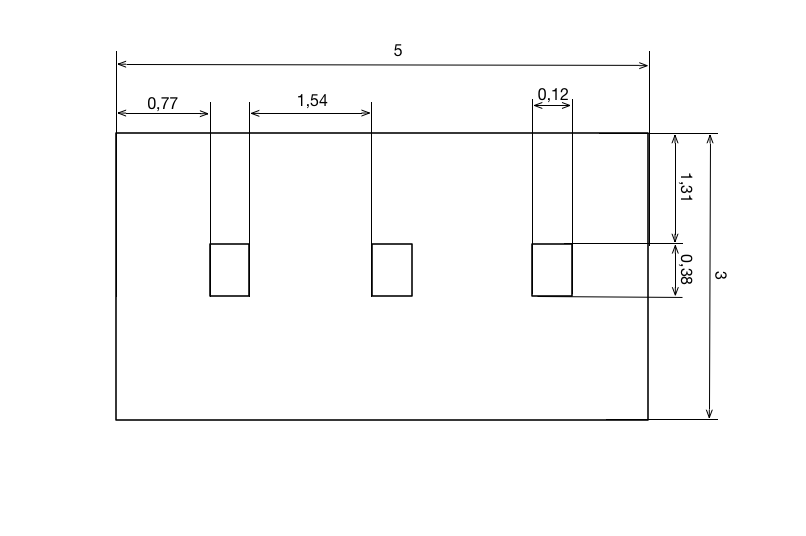
\includegraphics[width=0.8\linewidth]{pics/room.png}}
\caption{Схема расположения светильников в помещении операторов ПЭВМ.}
\label{pic:room}
\end{figure}
\subsection{Утилизация и списание аппаратных комплектующих}
Списание техники организация должна проводить, подтверждая факт утилизации компьютеров и оргтехники. Для организаций эта норма предписана Федеральным законом "Об отходах производства и потребления. То есть, списанная, но не утилизированная техника – это серьезное нарушение закона, не говоря уже об  угрозе окружающей среде.

\subsubsection{Стандартная процедура списания и утилизации техники}
Стандартный процесс списания техники и утилизации компьютерного оборудования включает в себя следующие шаги:
\begin{itemize}
\item Компания, перед которой стоит цель списания техники, создает специальную внутреннюю комиссию. Ее основной задачей будет принятие коллегиального решения о том, какую именно технику уже пора списывать.
\item Решение о списании компьютеров и оргтехники данной комиссии непременно должно базироваться на экспертном заключении. Эксперт может быть как штатным сотрудником компании (обязательно иметь подтверждающие документы по образованию в сфере обслуживания/ремонта данной техники), так и привлеченным извне независимым специалистом. Обязательно потребуется акт технической экспертизы компьютеров или оргтехники, проведенной компанией-производителем, либо другой компанией, имеющее разрешение на обслуживание и ремонт данной техники. Такой акт технической экспертизы компьютеров и оборудования документально подтверждает, что техника неисправна, ее ремонт нецелесообразен и ей пора на  покой. Можно списывать и утилизировать старую технику.
\item Чтобы окончательно завершить списание оргтехники и компьютеров и забыть о  них, придется предоставить еще и документальное подтверждение того, что он  действительно был правильно утилизирован, а не продолжил уничтожать нашу экосистему, распадаясь на тяжелые металлы и ядовитые соединения.

\end{itemize}

Очевидно, что данная процедура списания компьютеров и утилизации оборудования очень долгая и сложная. Правильней было бы заключить договор на утилизацию и перепоручить  утилизацию оборудования специализированной компании.

Компании предлагают услугу вывоза и утилизации компьютерной техники и оргтехники, которая поможет быстро, законно и с минимальными затратами сил и времени избавиться от старой техники. 

После заключения договора, специализированная компания несет ответственность за то, чтобы провести правильное списание оргтехники и корректно выполнить вывоз и утилизацию компьютеров и прочей старой техники.
При утилизации старых компьютеров происходит их разработк
а на фракции: металлы, пластмассы, стекло, провода, штекеры. Из одной тонны компьютерного лома получают до 200 кг меди, 480 кг железа и нержавеющей стали, 32 кг алюминия, 3 кг серебра, 1 кг золота и 300 г палладия.

Переработку промышленных отходов производят на специальных полигонах, создаваемых в соответствии с требованиями СНиП 2.01.28-85 и предназначенных для централизованного сбора обезвреживания и захоронения токсичных отходов промышленных предприятий, НИИ и учреждений.
                       
\newpage
\section*{Заключение}
\addcontentsline{toc}{section}{Заключение}
В результате выполнения дипломного проекта решены следующие задачи:
\begin{itemize}
\item проведено исследование предметной области, выбраны и обоснованы критерии качества системы;
\item разработана структура подсистемы, произведен анализ аналогов системы;
\item проработана математическая модель;
\item разработана архитектура системы;
\item разработана тестовая версия подсистемы;
\item произведено исследование зависимости времени вычисления оптического потока разными методами в зависимости от разных параметров;
\item разработаны рекомендации по организации рабочего места разработчика подсистемы;
\item рассчитаны затраты на разработку и тестирование системы;
\item разработана графическая часть документации в составе 10 листов формата А1.
\end{itemize}
Разработанная подсистема является важным структурным компонентом для различных систем управления подвижными объектами.


\newpage
\addcontentsline{toc}{section}{Список используемых источников}
\bibliographystyle{utf8gost705u}
\renewcommand\bibname{Список используемых источников}
\section*{\bibname}
\bibliography{biblio}

\newpage
\appendix

%\addcontentsline{toc}{section}{Приложение А Техническое задание}
\section{Техническое задание}

\newpage
\setcounter{page}{121}
\section{Графическая часть}

\newpage
\begin{figure}[H]
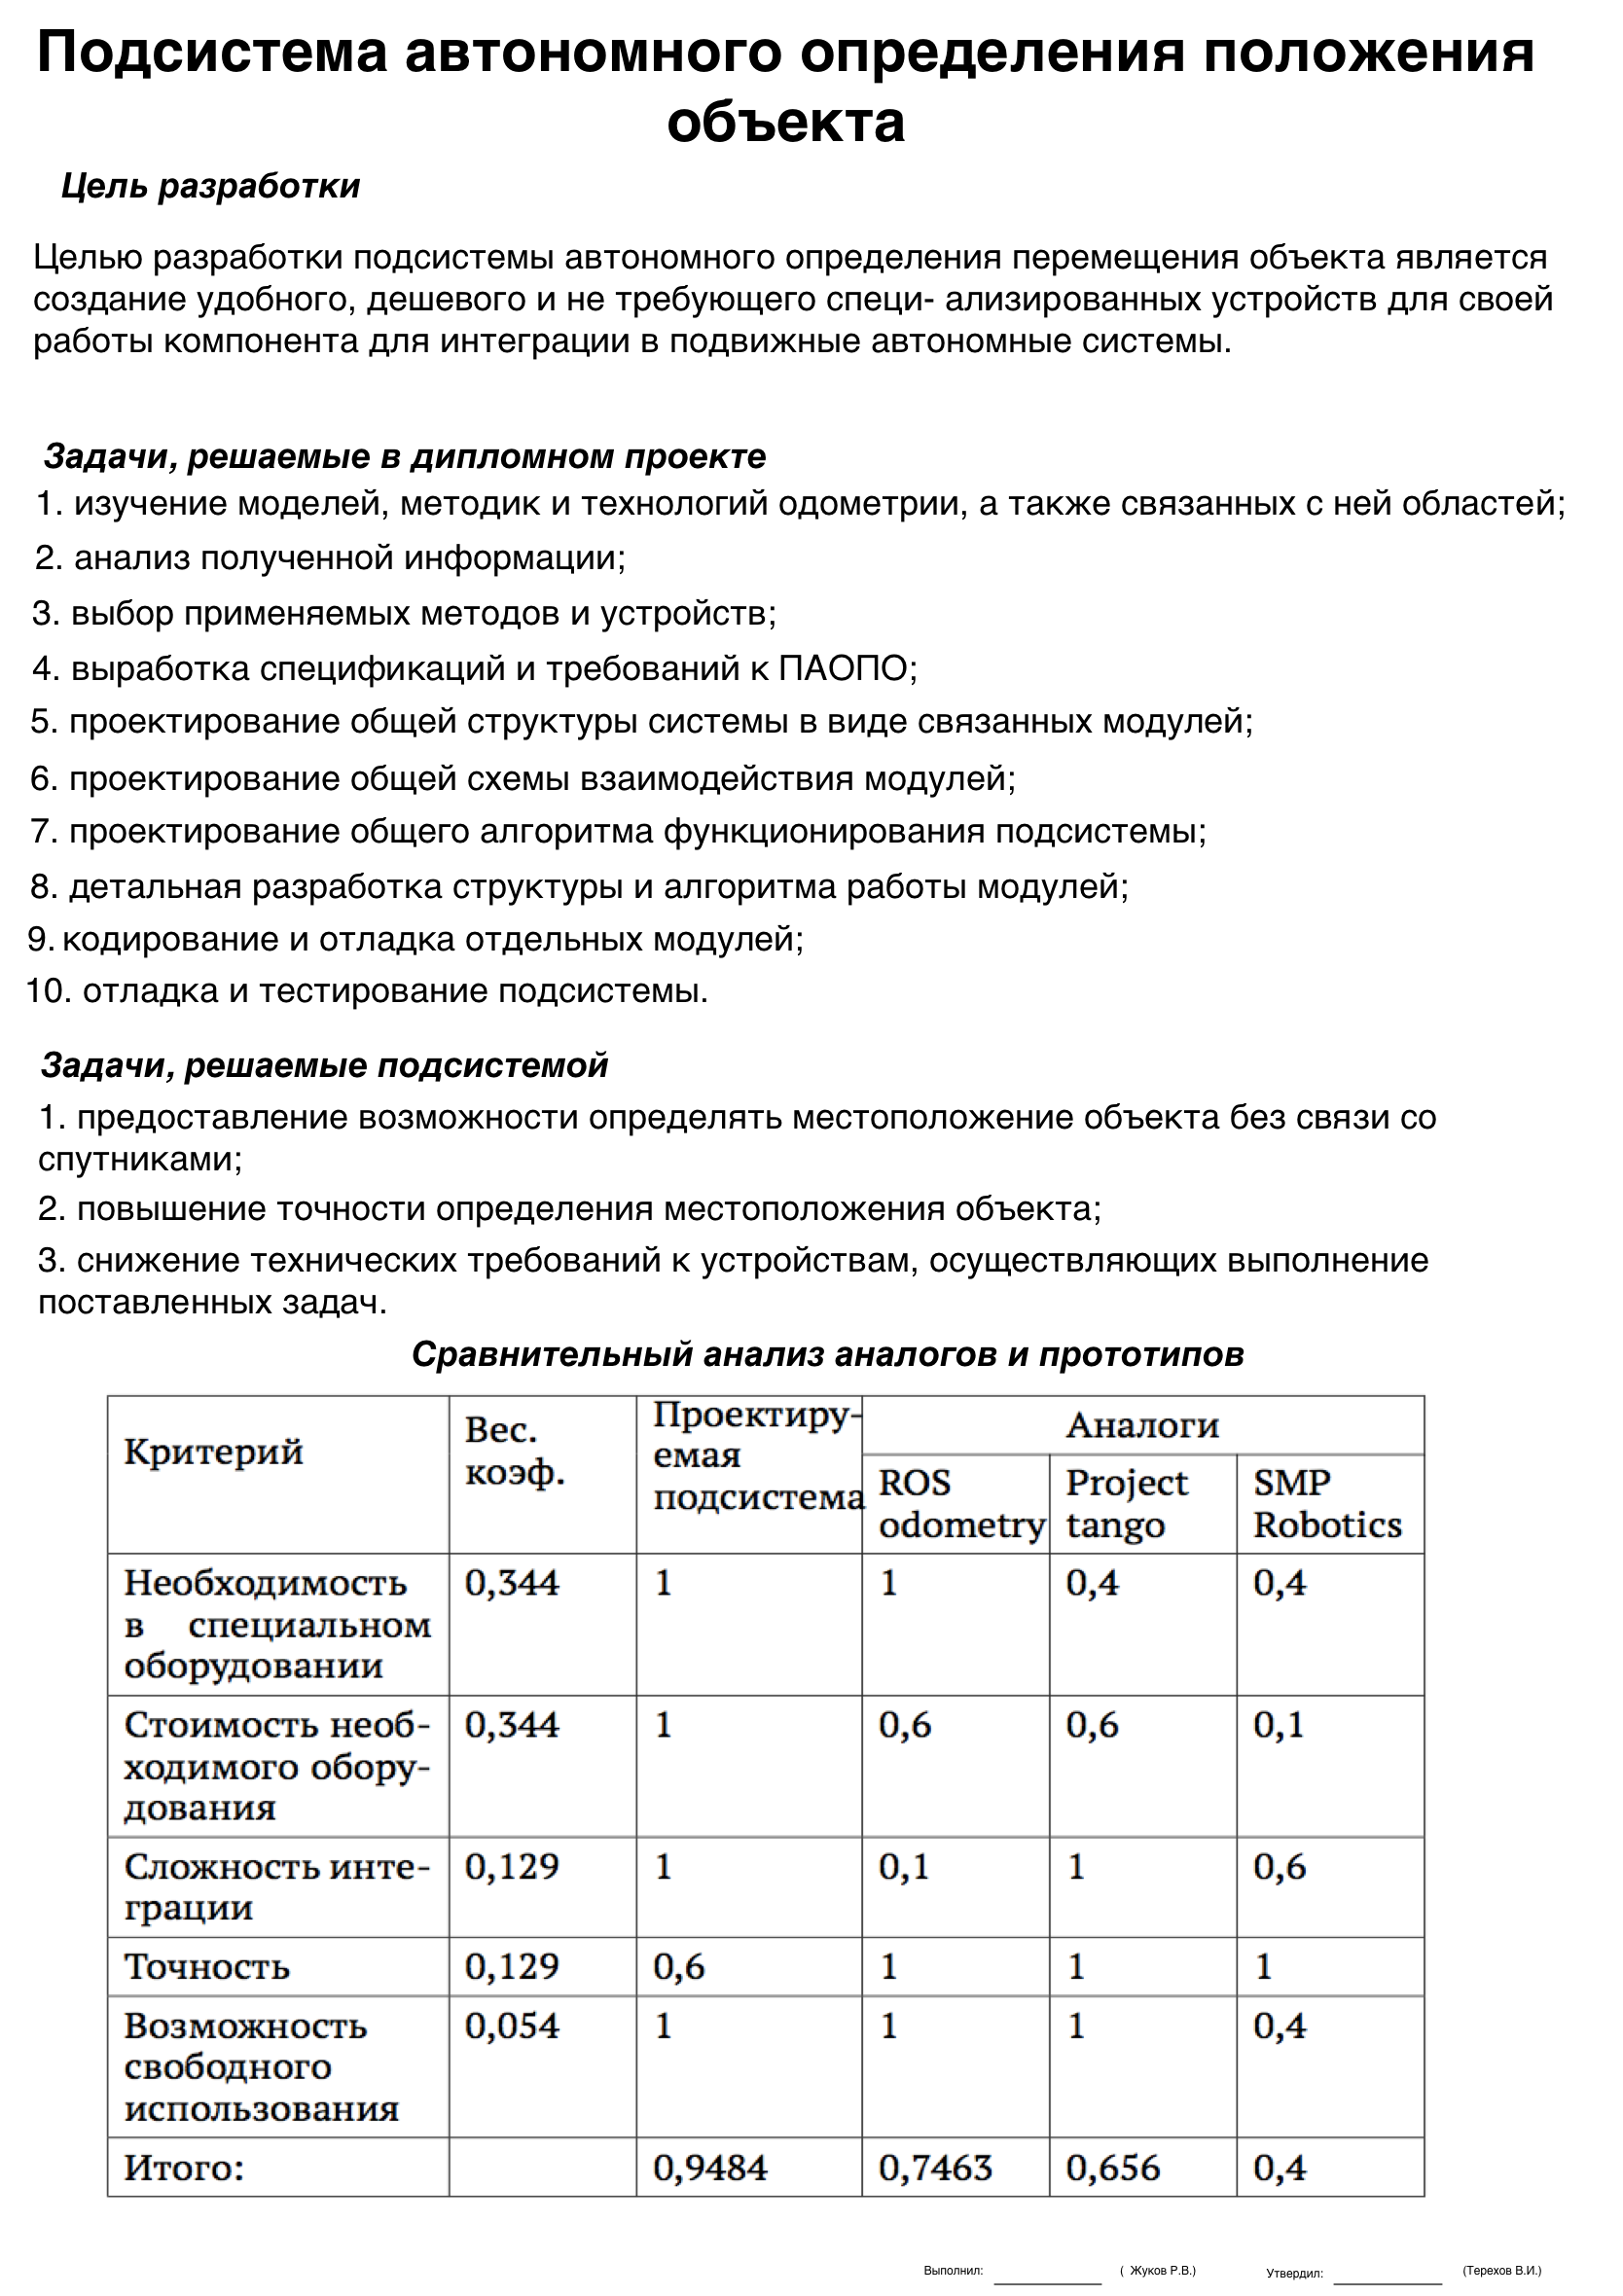
\includegraphics[width=0.99\linewidth]{pics/G1.png}
\end{figure}

\afterpage{
%\thispagestyle{empty}
\begin{landscape}
	\begin{figure}[!ht]
	\center{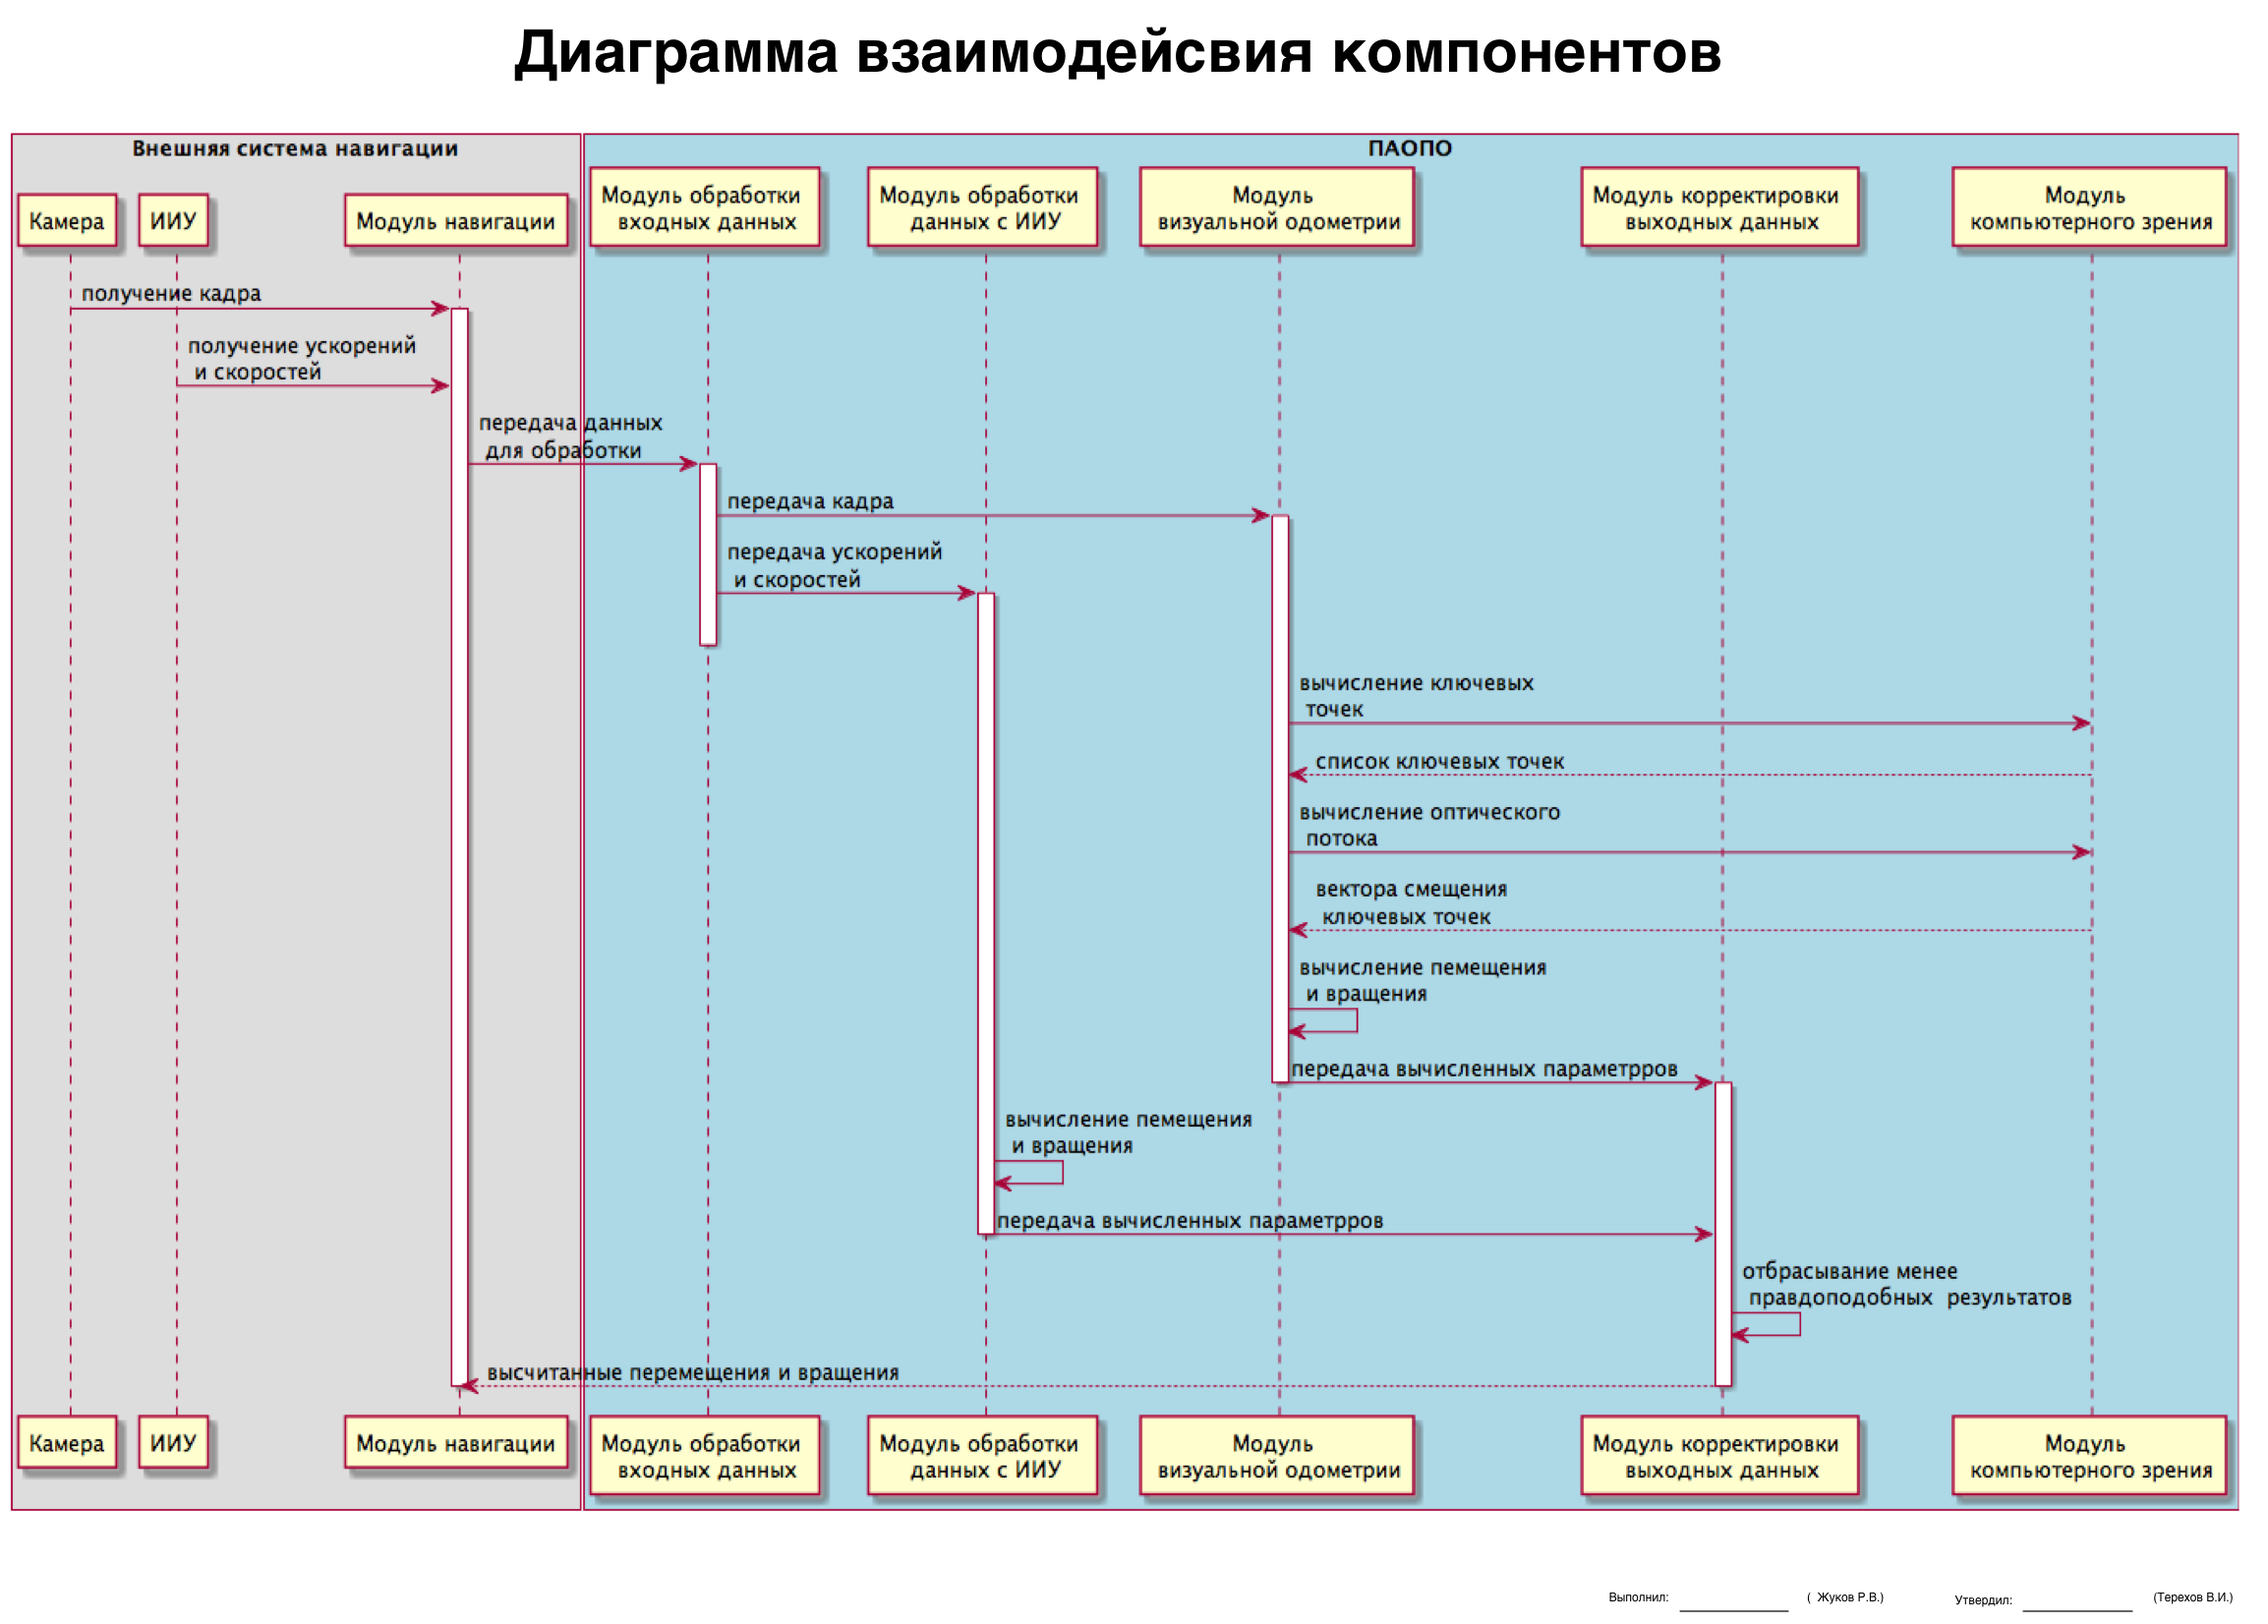
\includegraphics[width=0.99\linewidth]{pics/G2.png}}
\end{figure}
\end{landscape}
\clearpage
}

\afterpage{
%\thispagestyle{empty}
\begin{landscape}
	\begin{figure}[!ht]
	\center{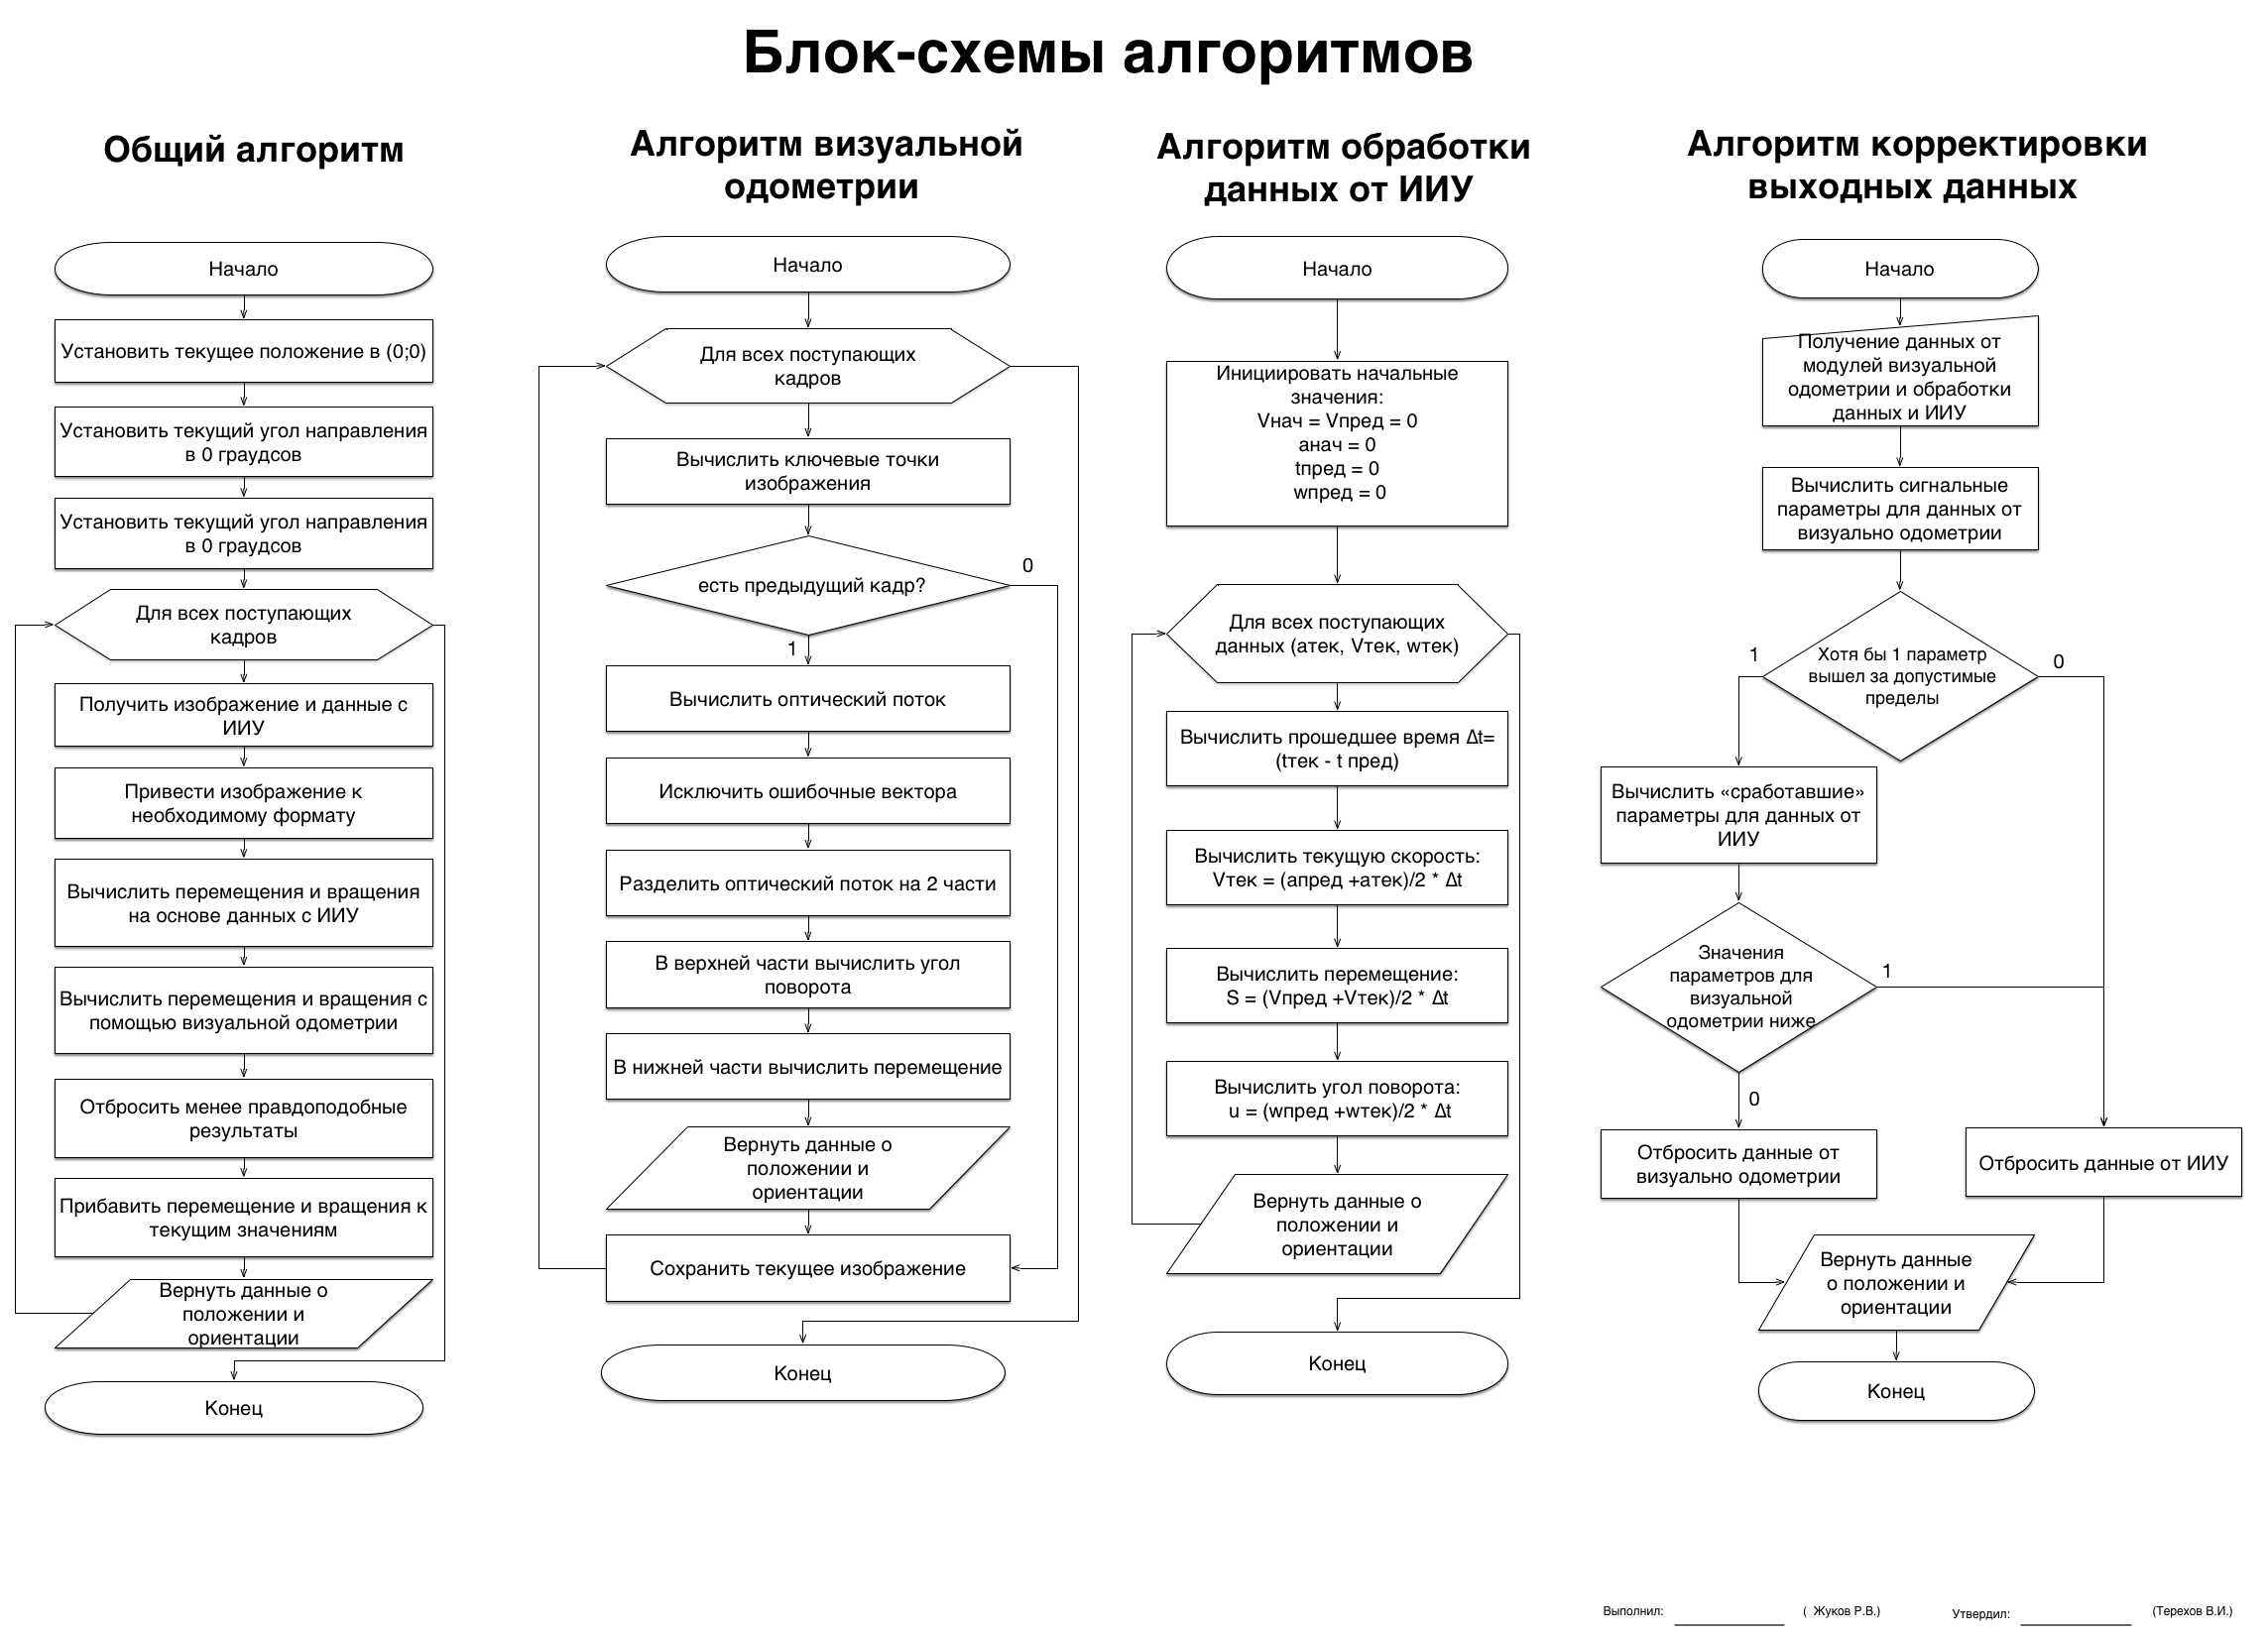
\includegraphics[width=0.99\linewidth]{pics/G3.png}}
\end{figure}
\end{landscape}
\clearpage
}

\begin{figure}[H]
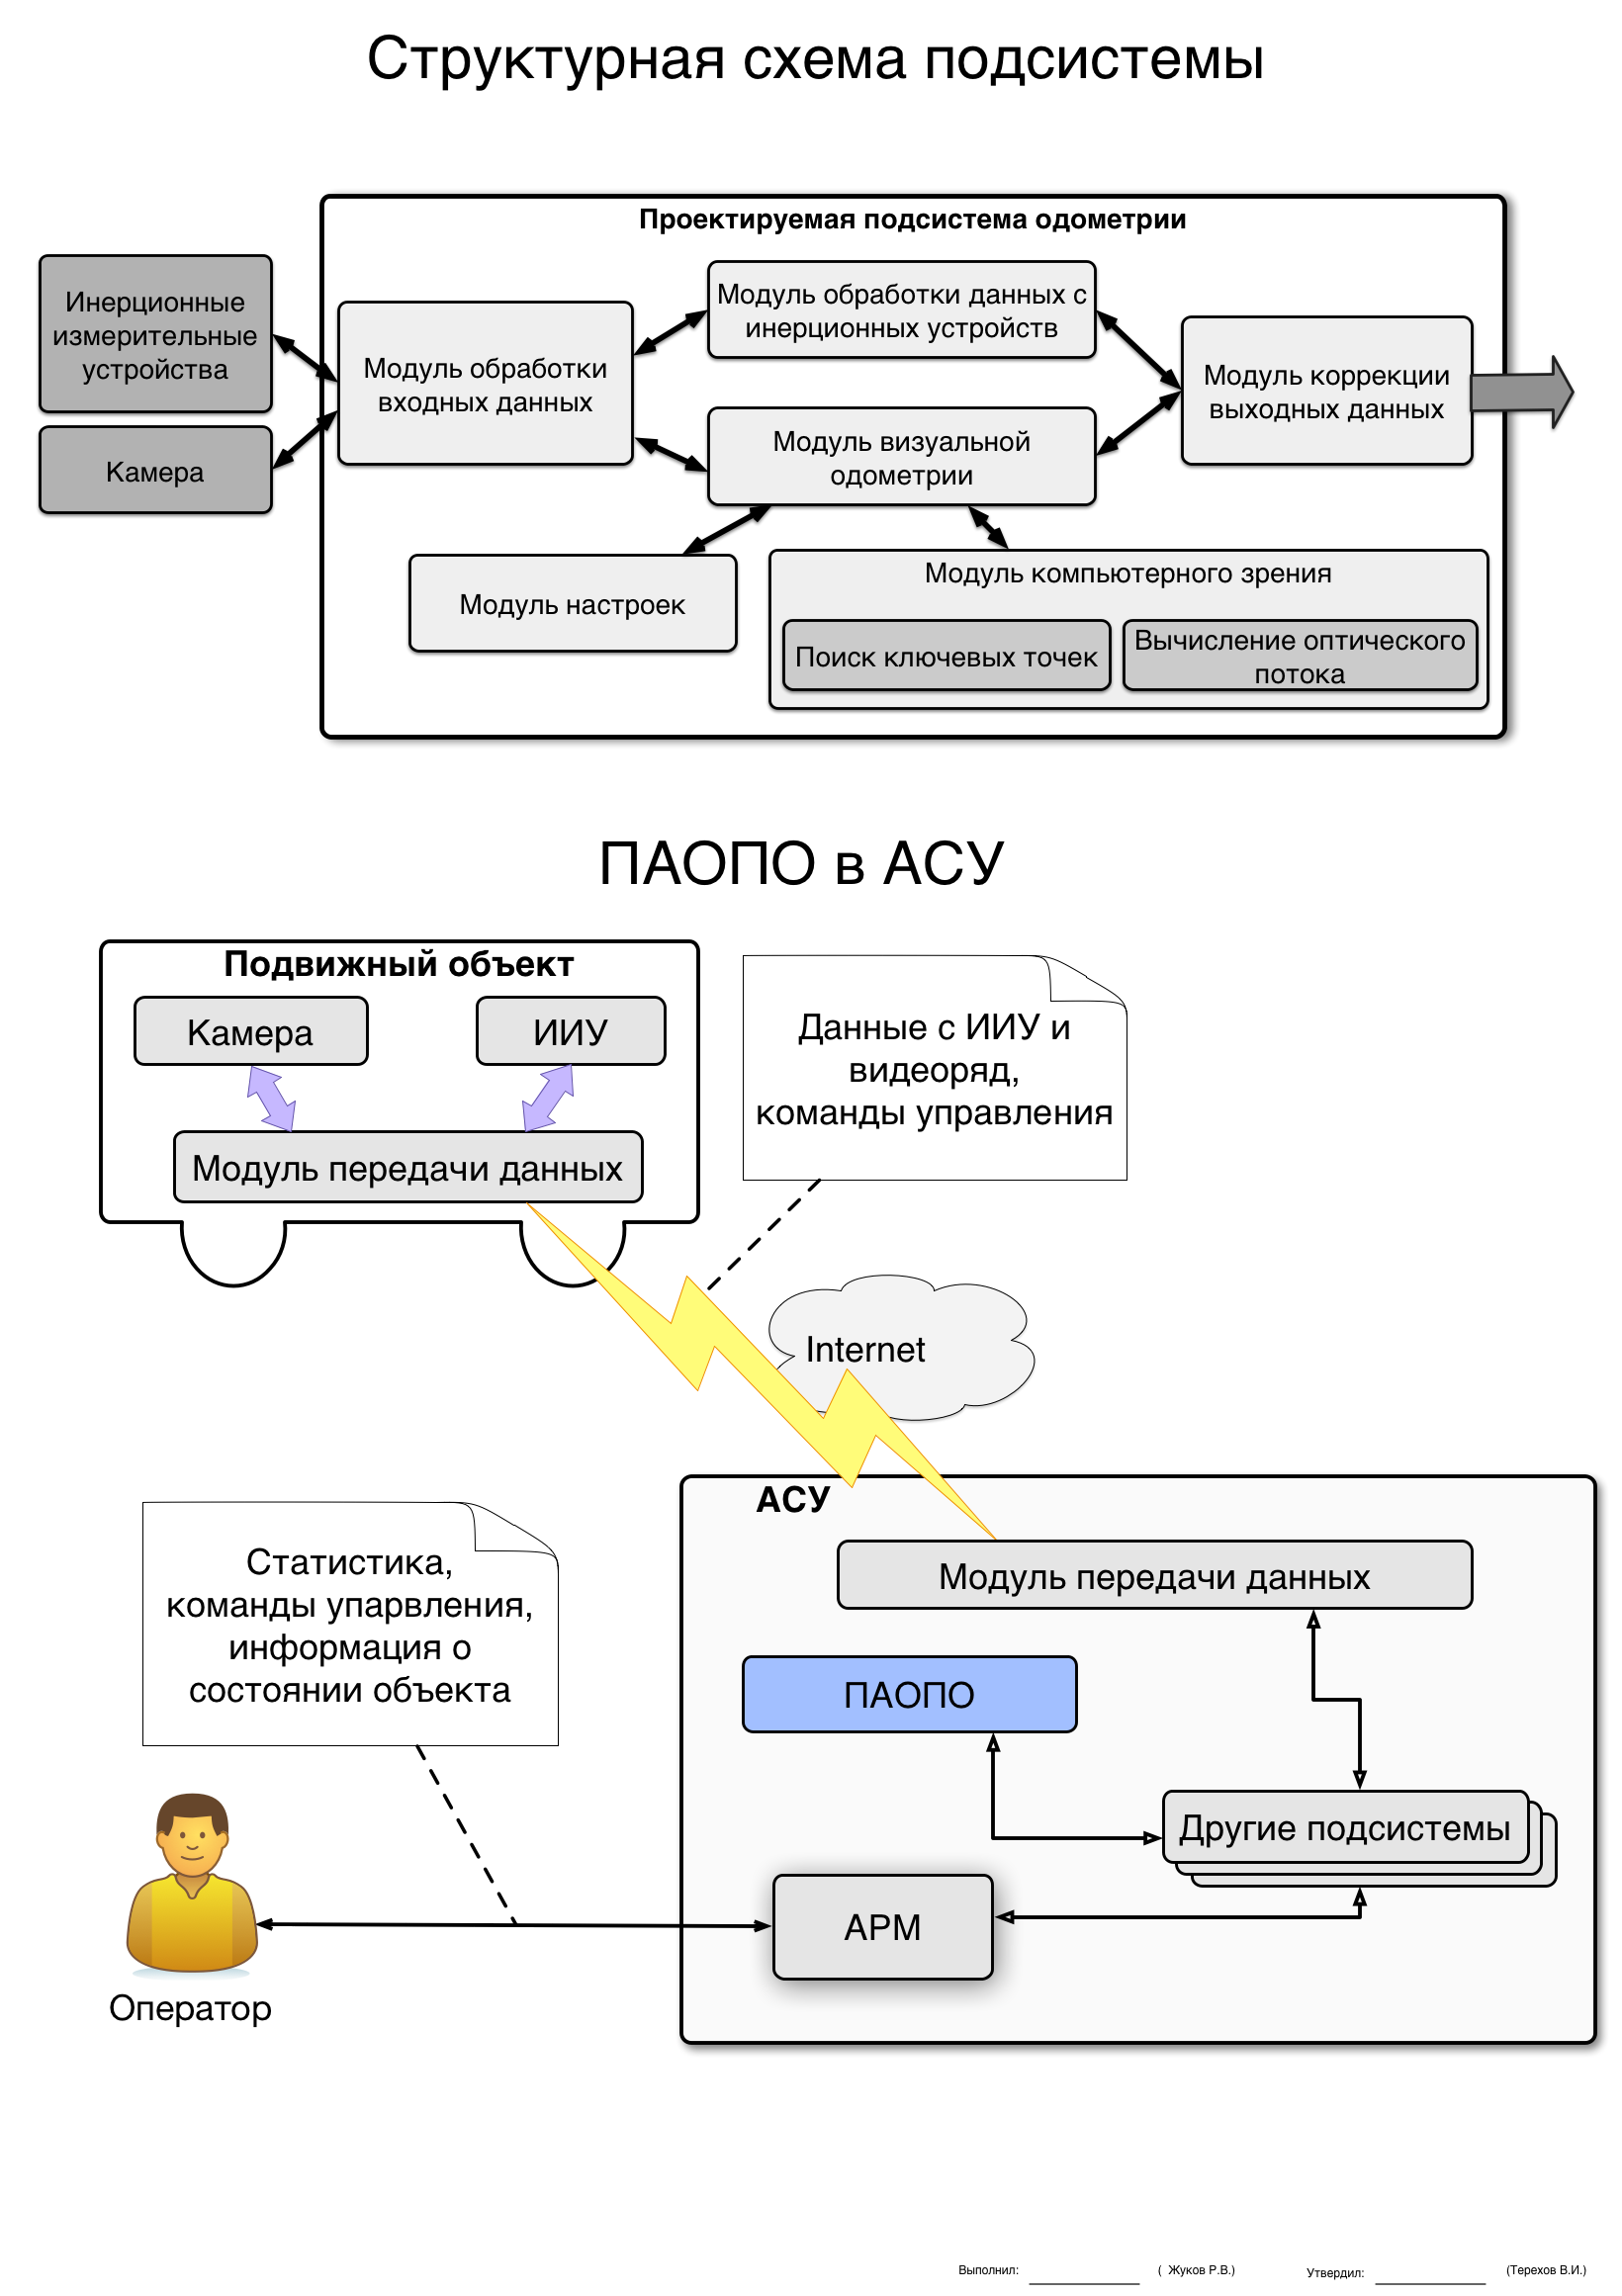
\includegraphics[width=0.99\linewidth]{pics/G4.png}
\end{figure}

\afterpage{
%\thispagestyle{empty}
\begin{landscape}
	\begin{figure}[!ht]
	\center{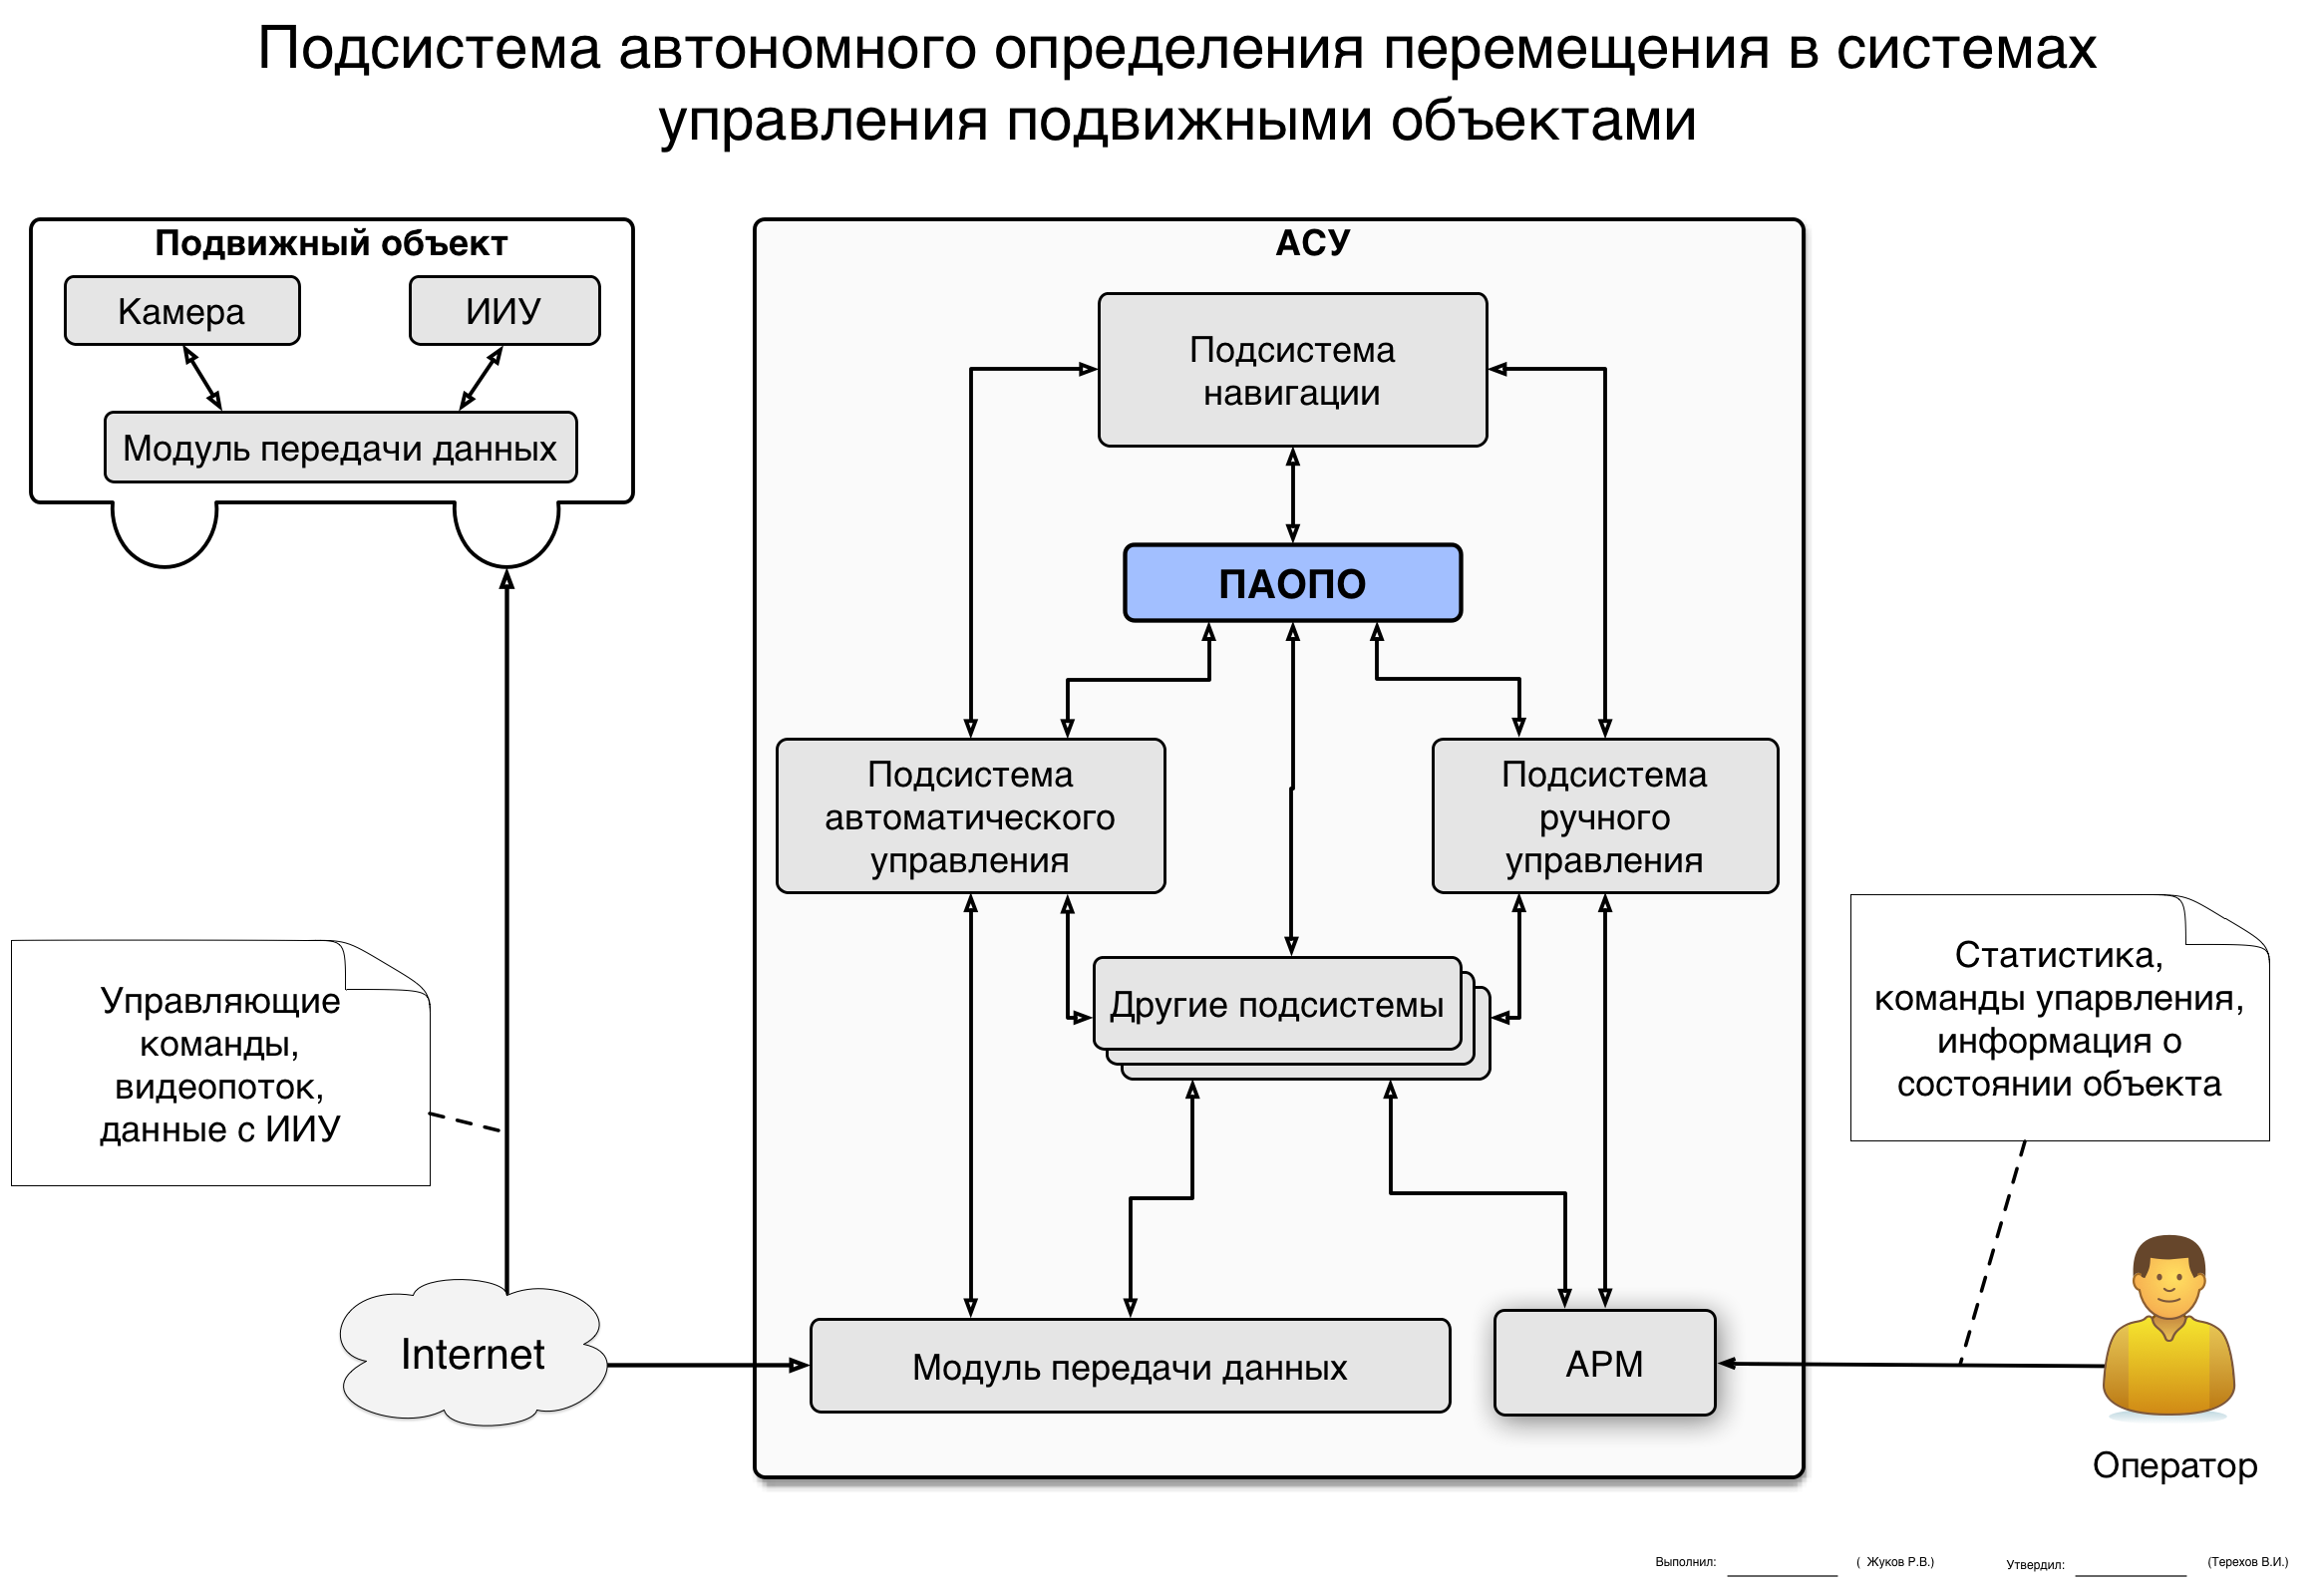
\includegraphics[width=0.99\linewidth]{pics/G5.png}}
\end{figure}
\end{landscape}
\clearpage
}

\afterpage{
%\thispagestyle{empty}
\begin{landscape}
	\begin{figure}[!ht]
	\center{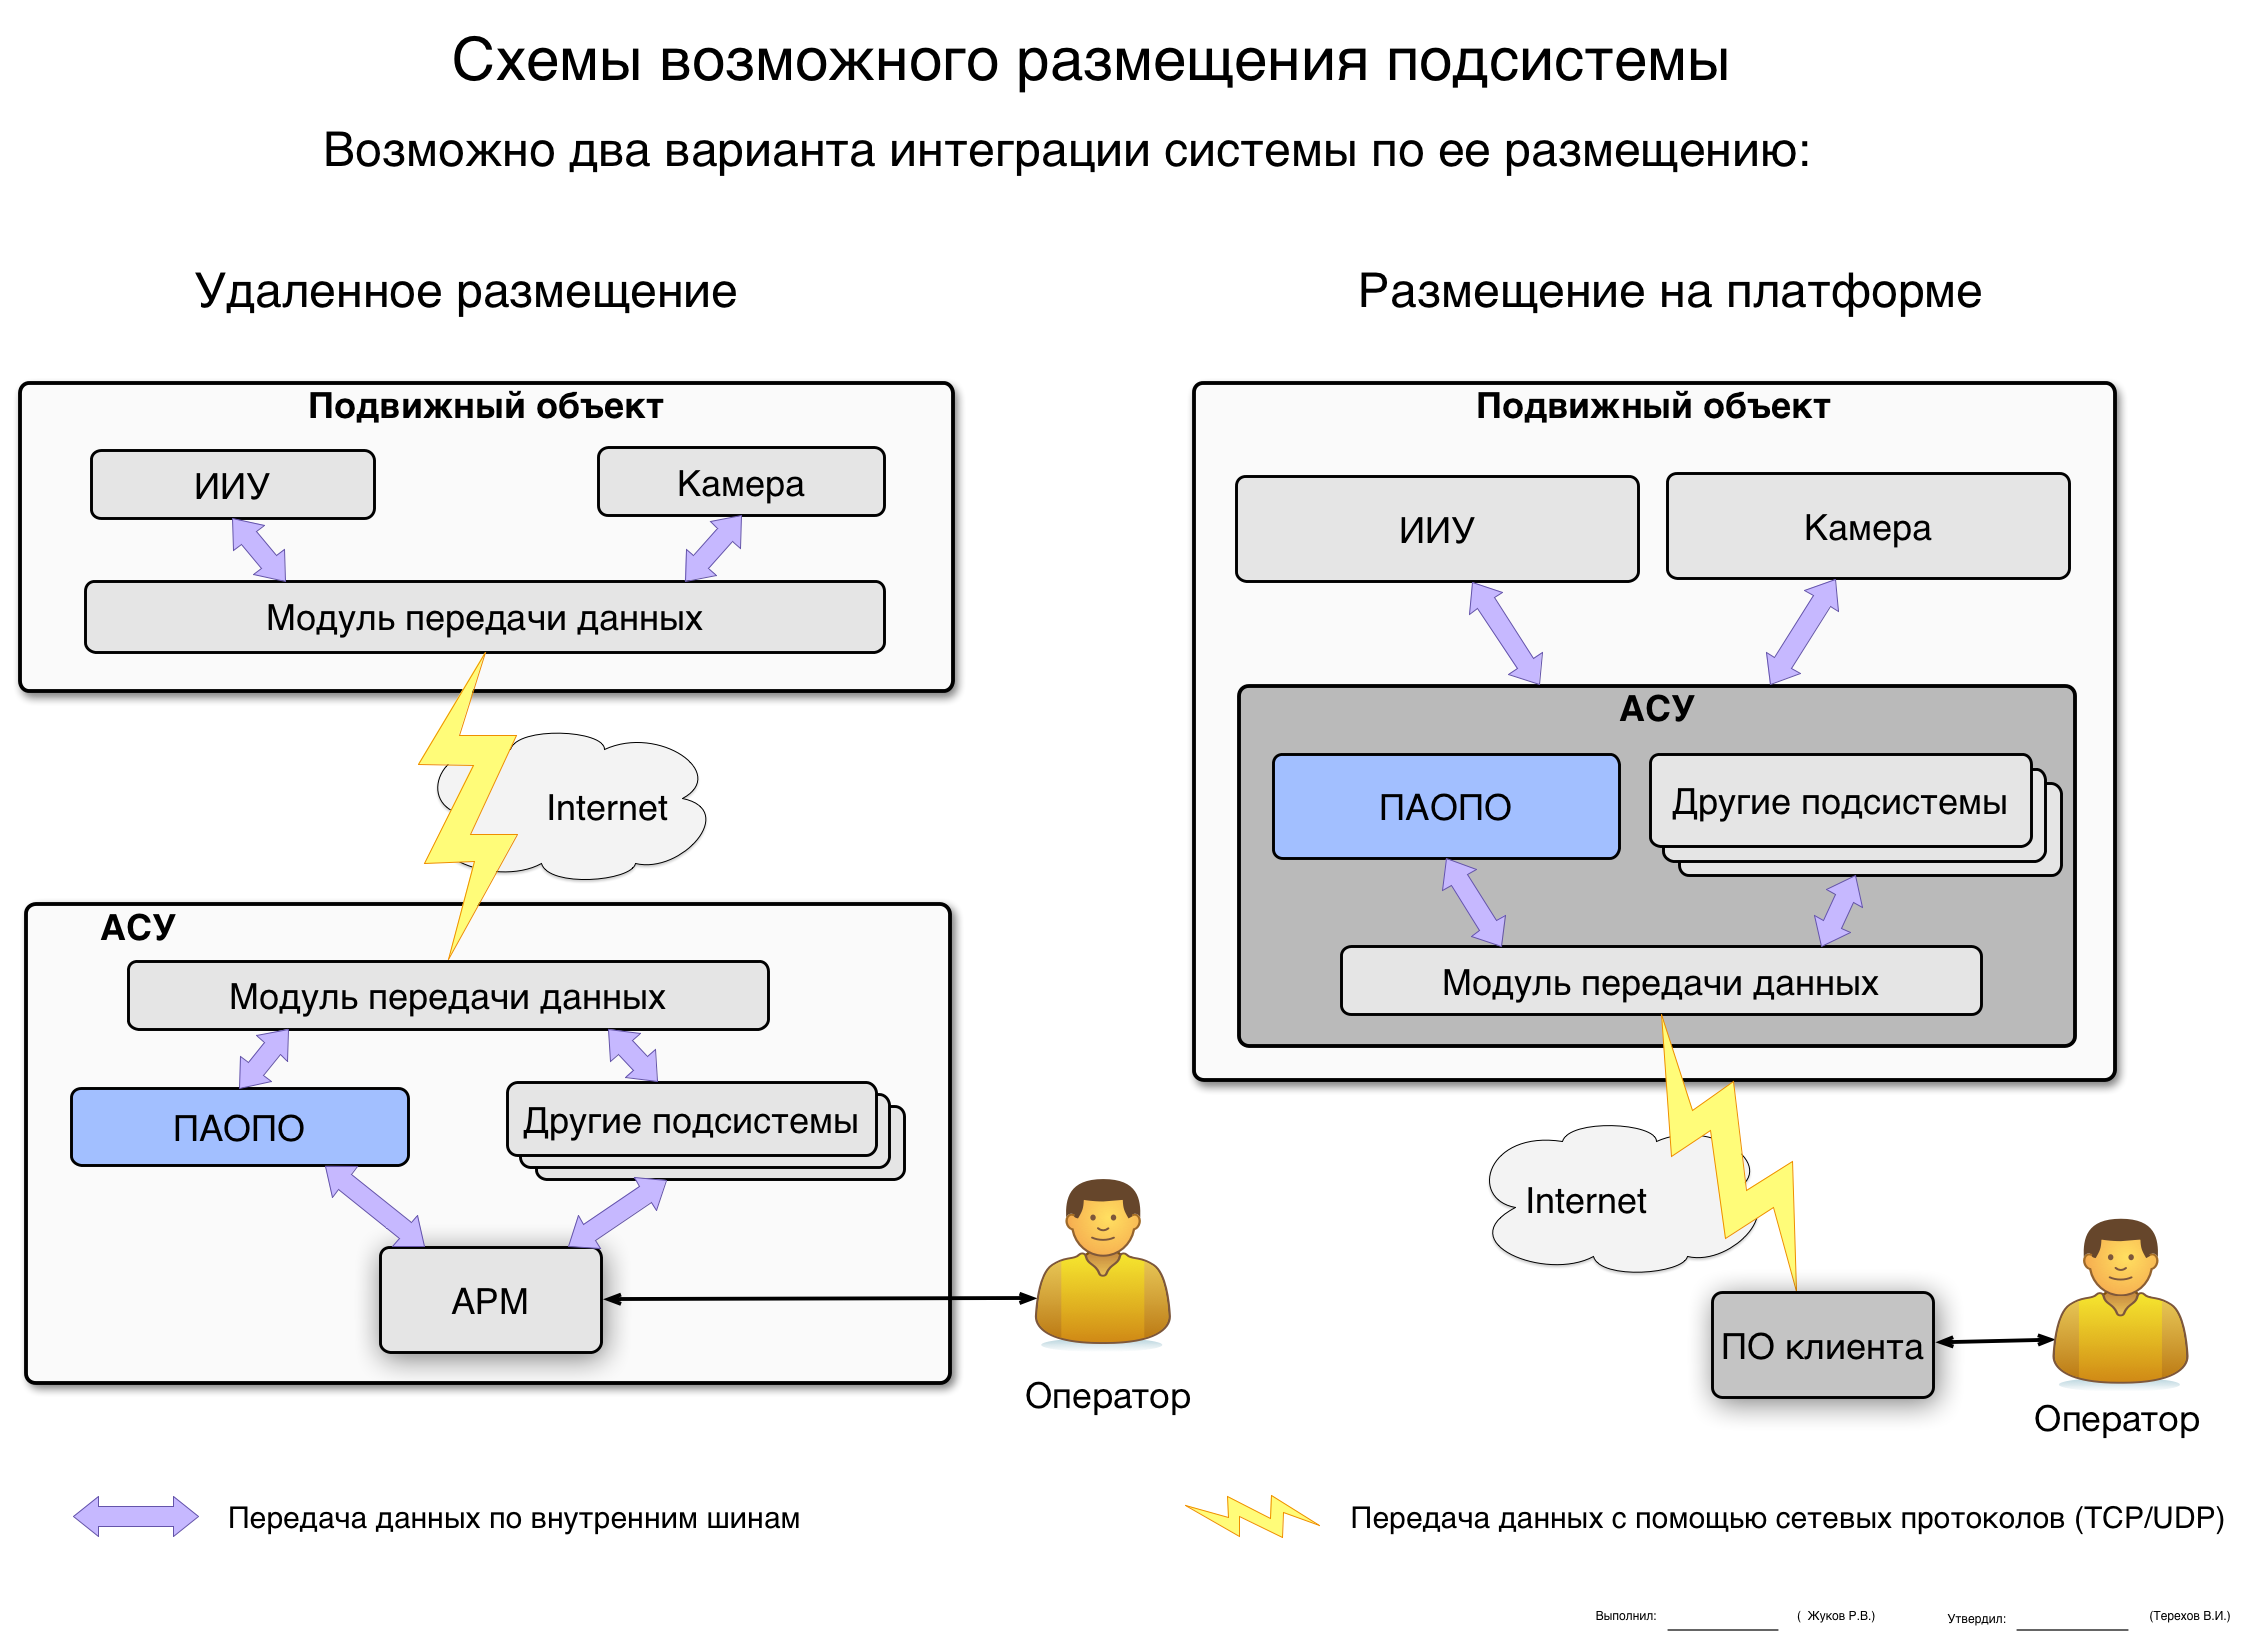
\includegraphics[width=0.99\linewidth]{pics/G6.png}}
\end{figure}
\end{landscape}
\clearpage
}

\begin{figure}[H]
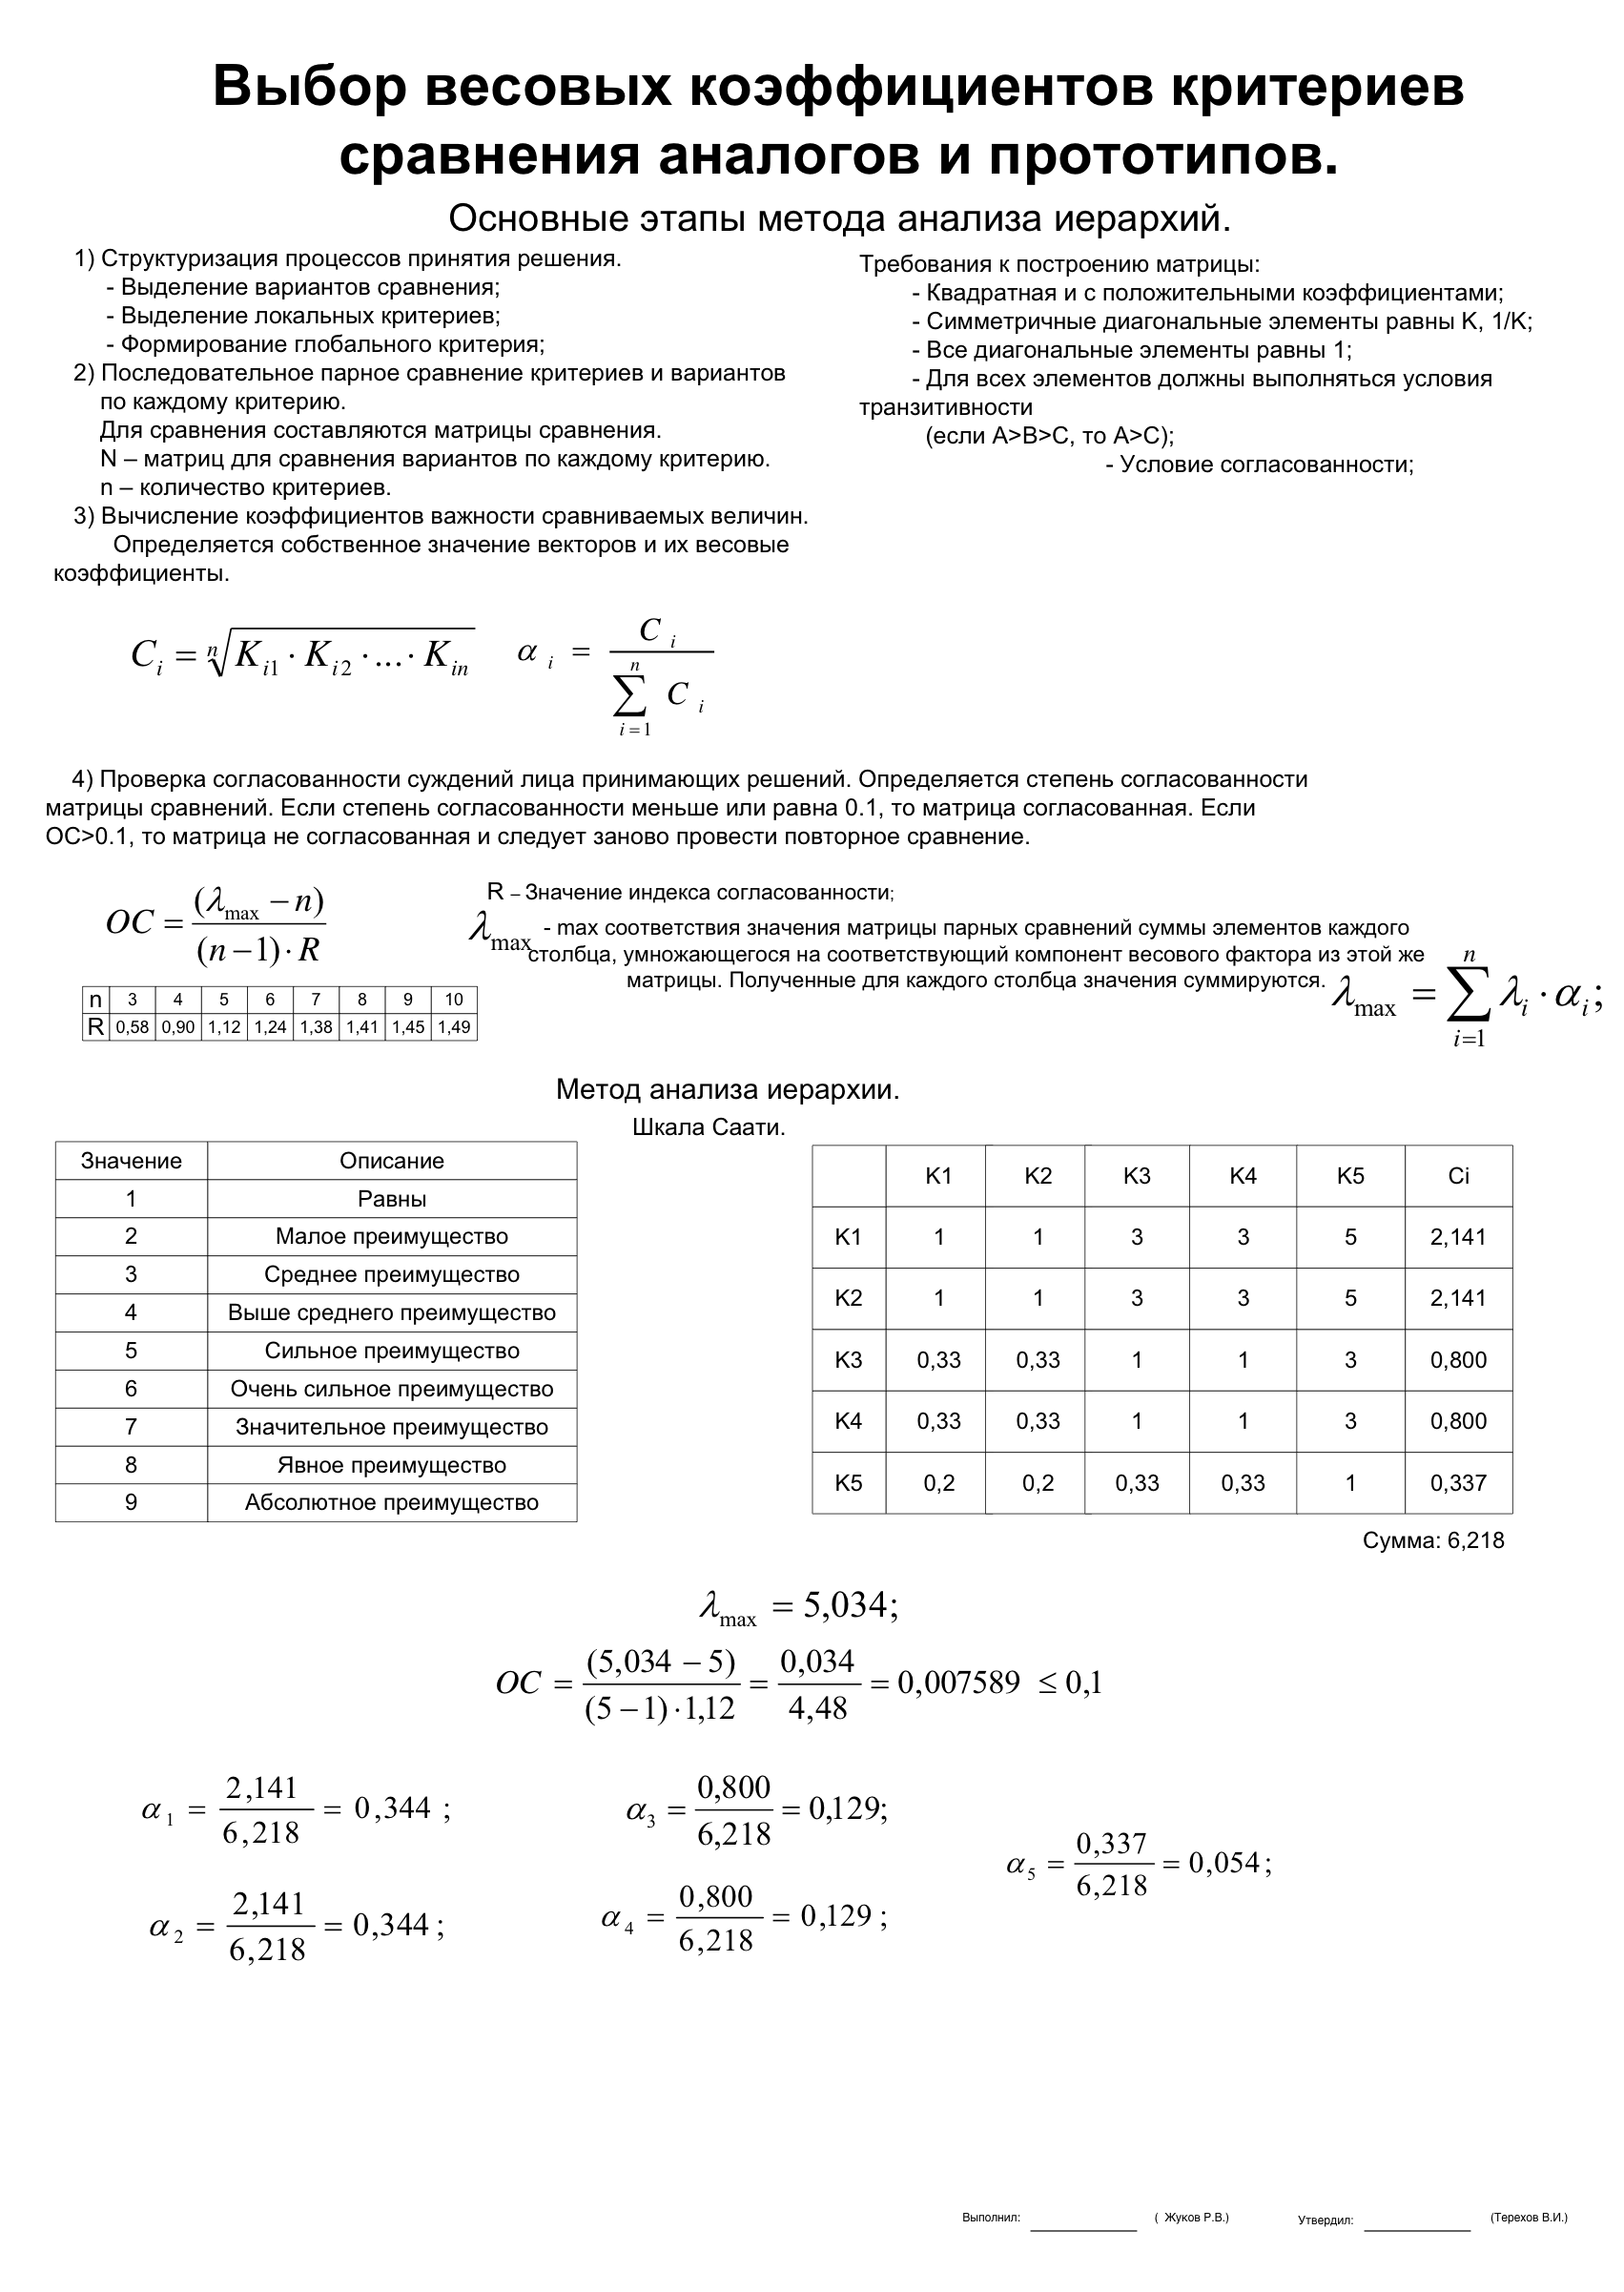
\includegraphics[width=0.99\linewidth]{pics/G7.png}
\end{figure}

\afterpage{
%\thispagestyle{empty}
\begin{landscape}
	\begin{figure}[!ht]
	\center{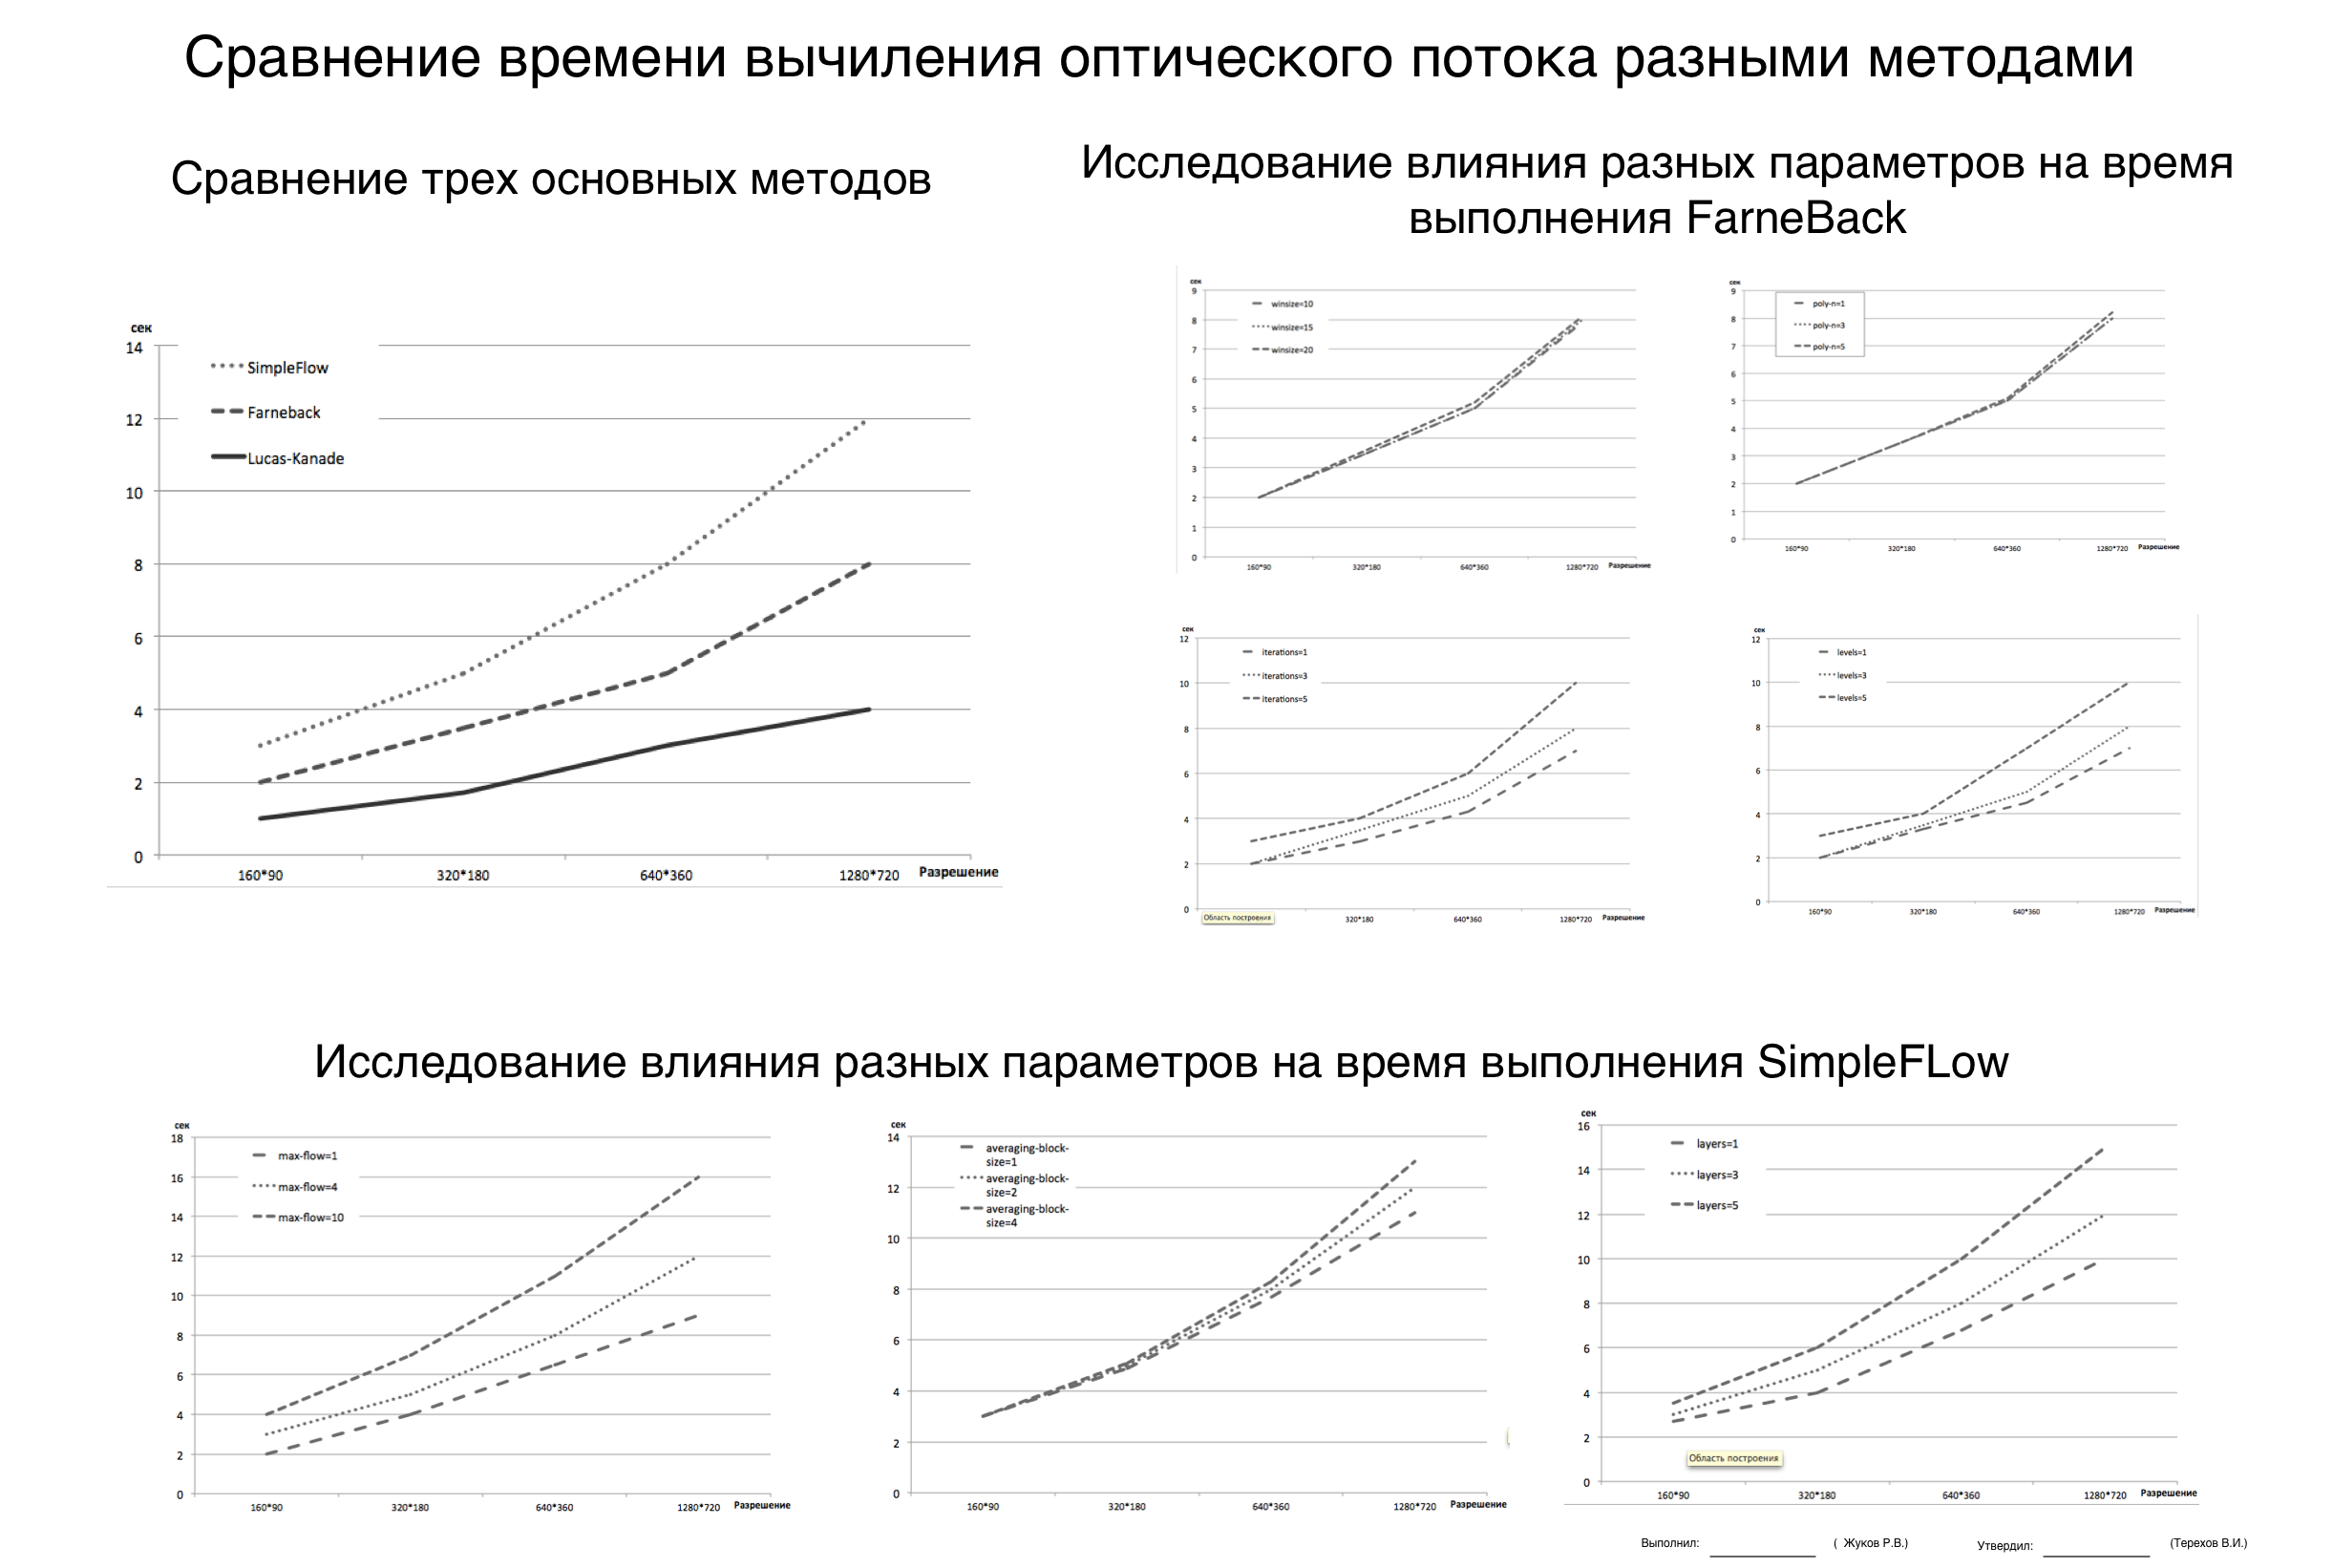
\includegraphics[width=0.99\linewidth]{pics/G8.png}}
\end{figure}
\end{landscape}
\clearpage
}

\afterpage{
%\thispagestyle{empty}
\begin{landscape}
	\begin{figure}[!ht]
	\center{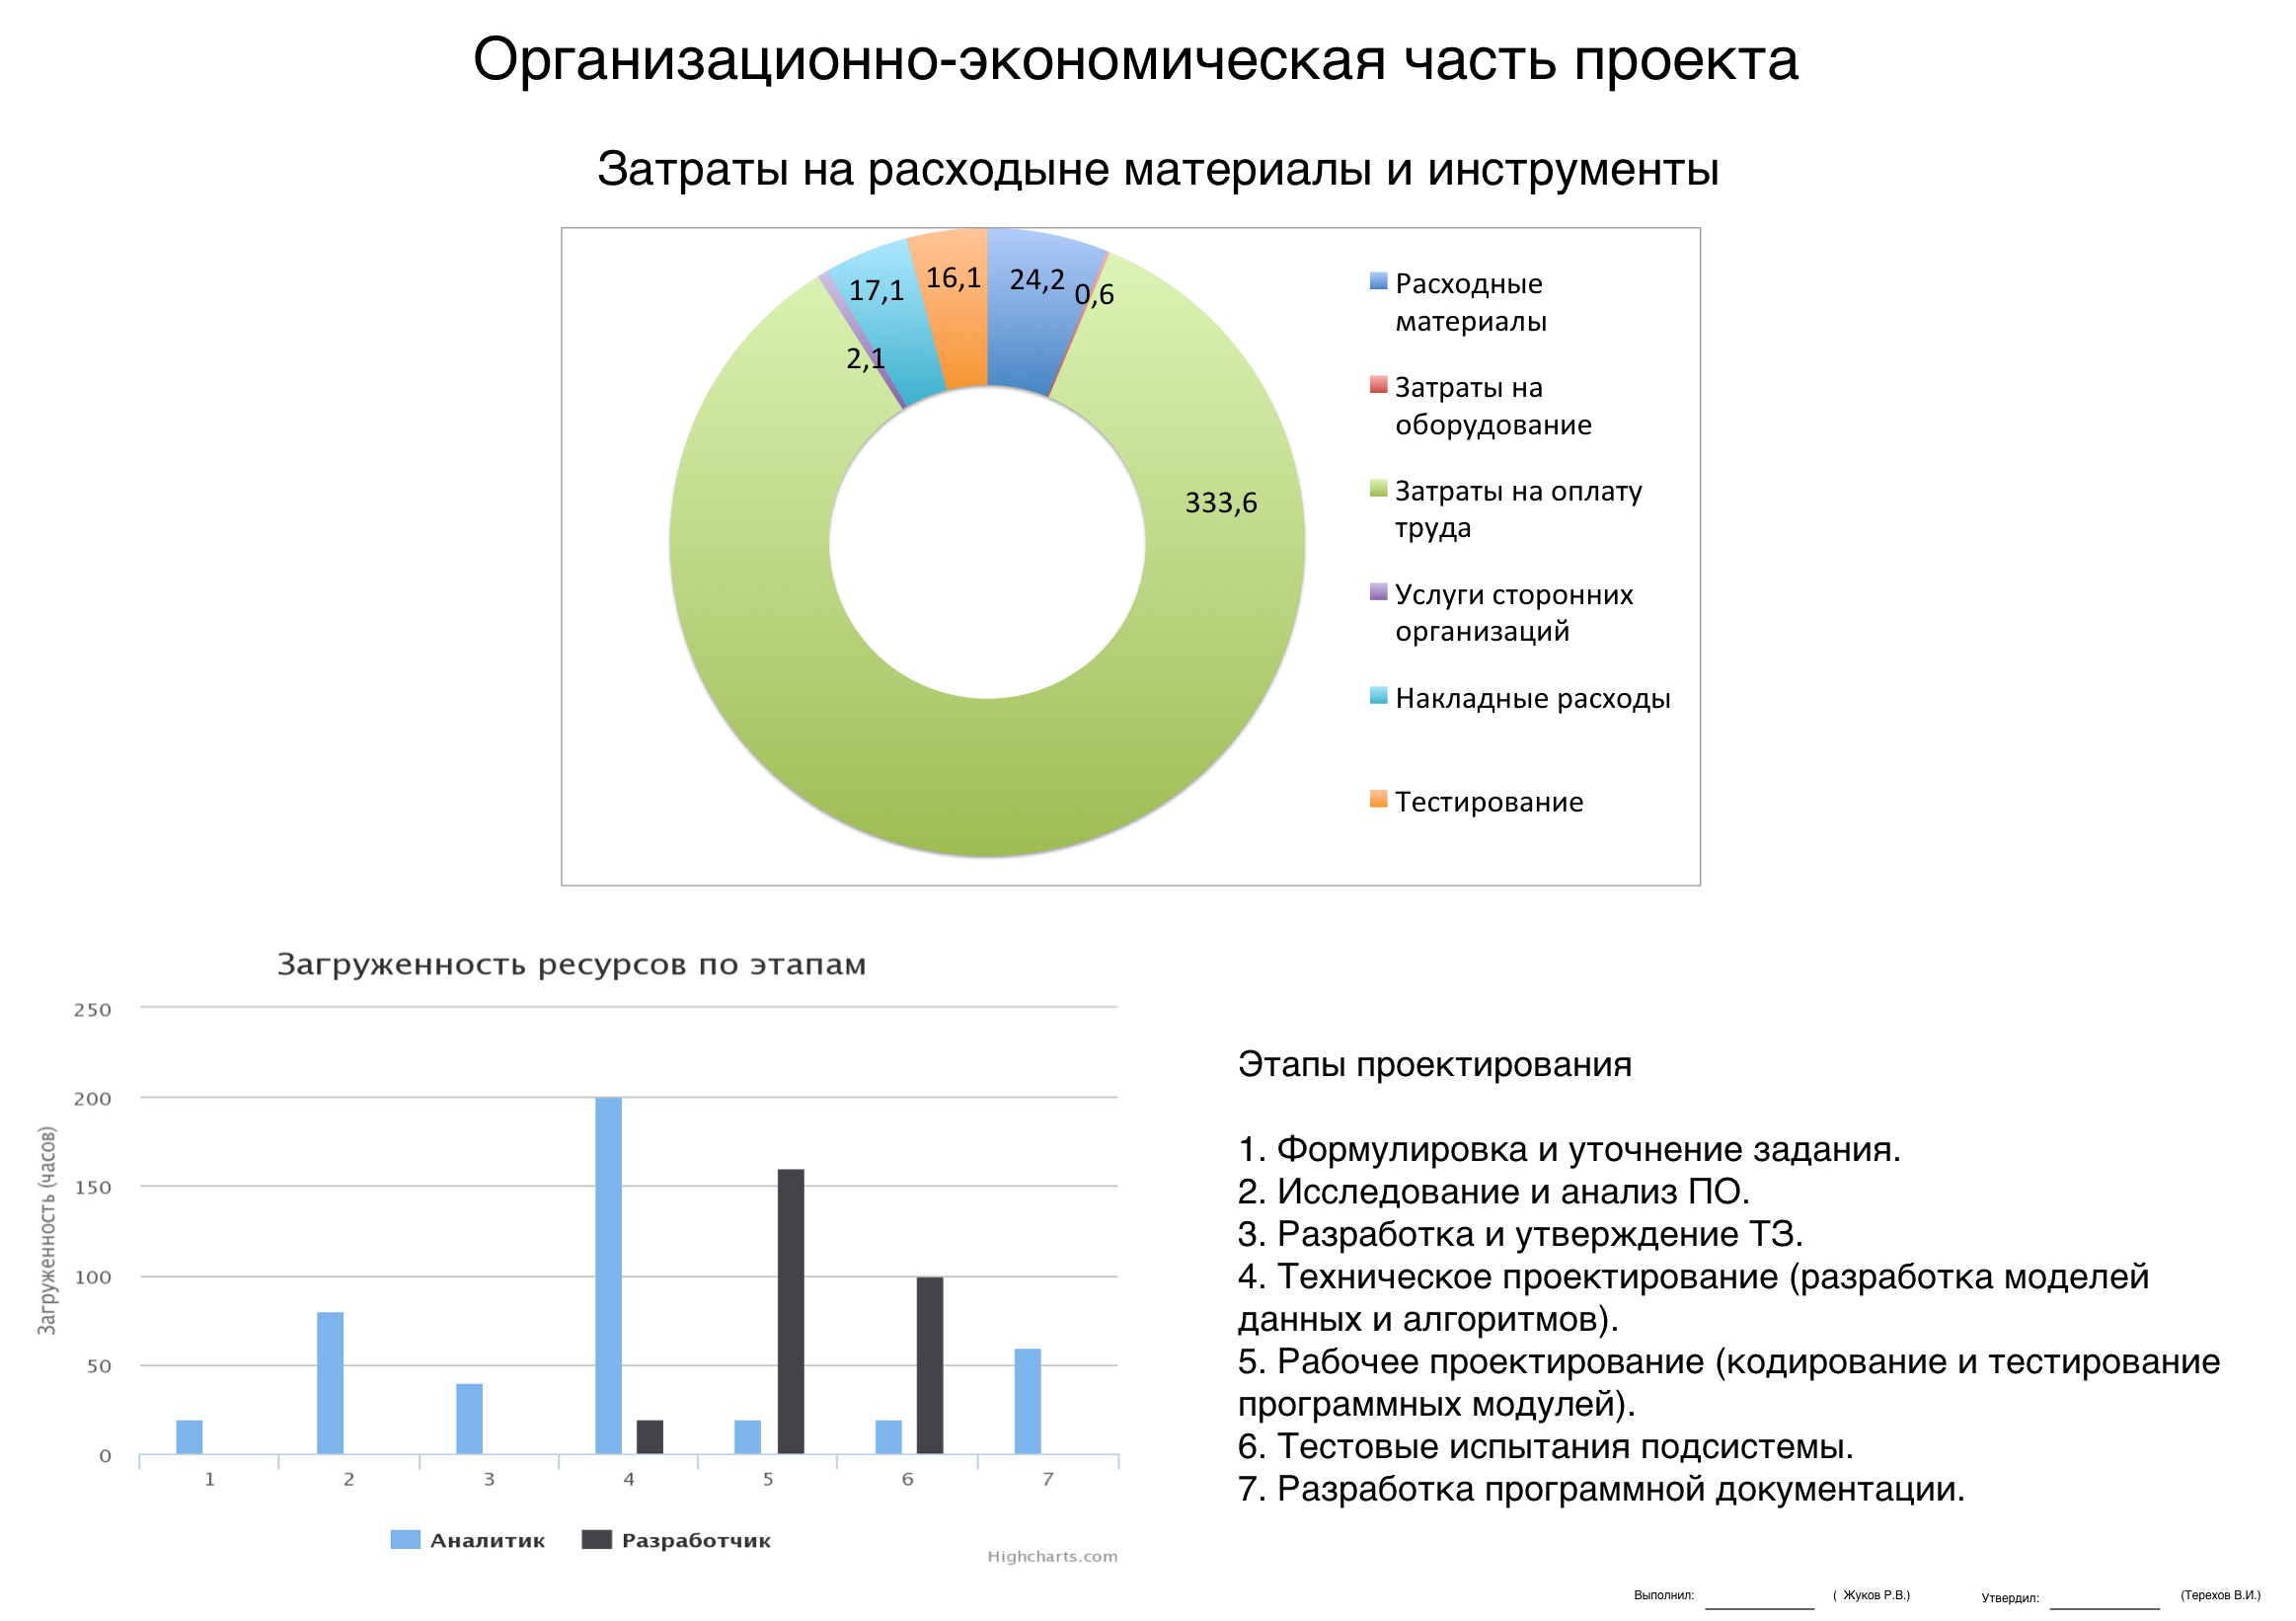
\includegraphics[width=0.99\linewidth]{pics/G9.png}}
\end{figure}
\end{landscape}
\clearpage
}

\afterpage{
%\thispagestyle{empty}
\begin{landscape}
	\begin{figure}[!ht]
	\center{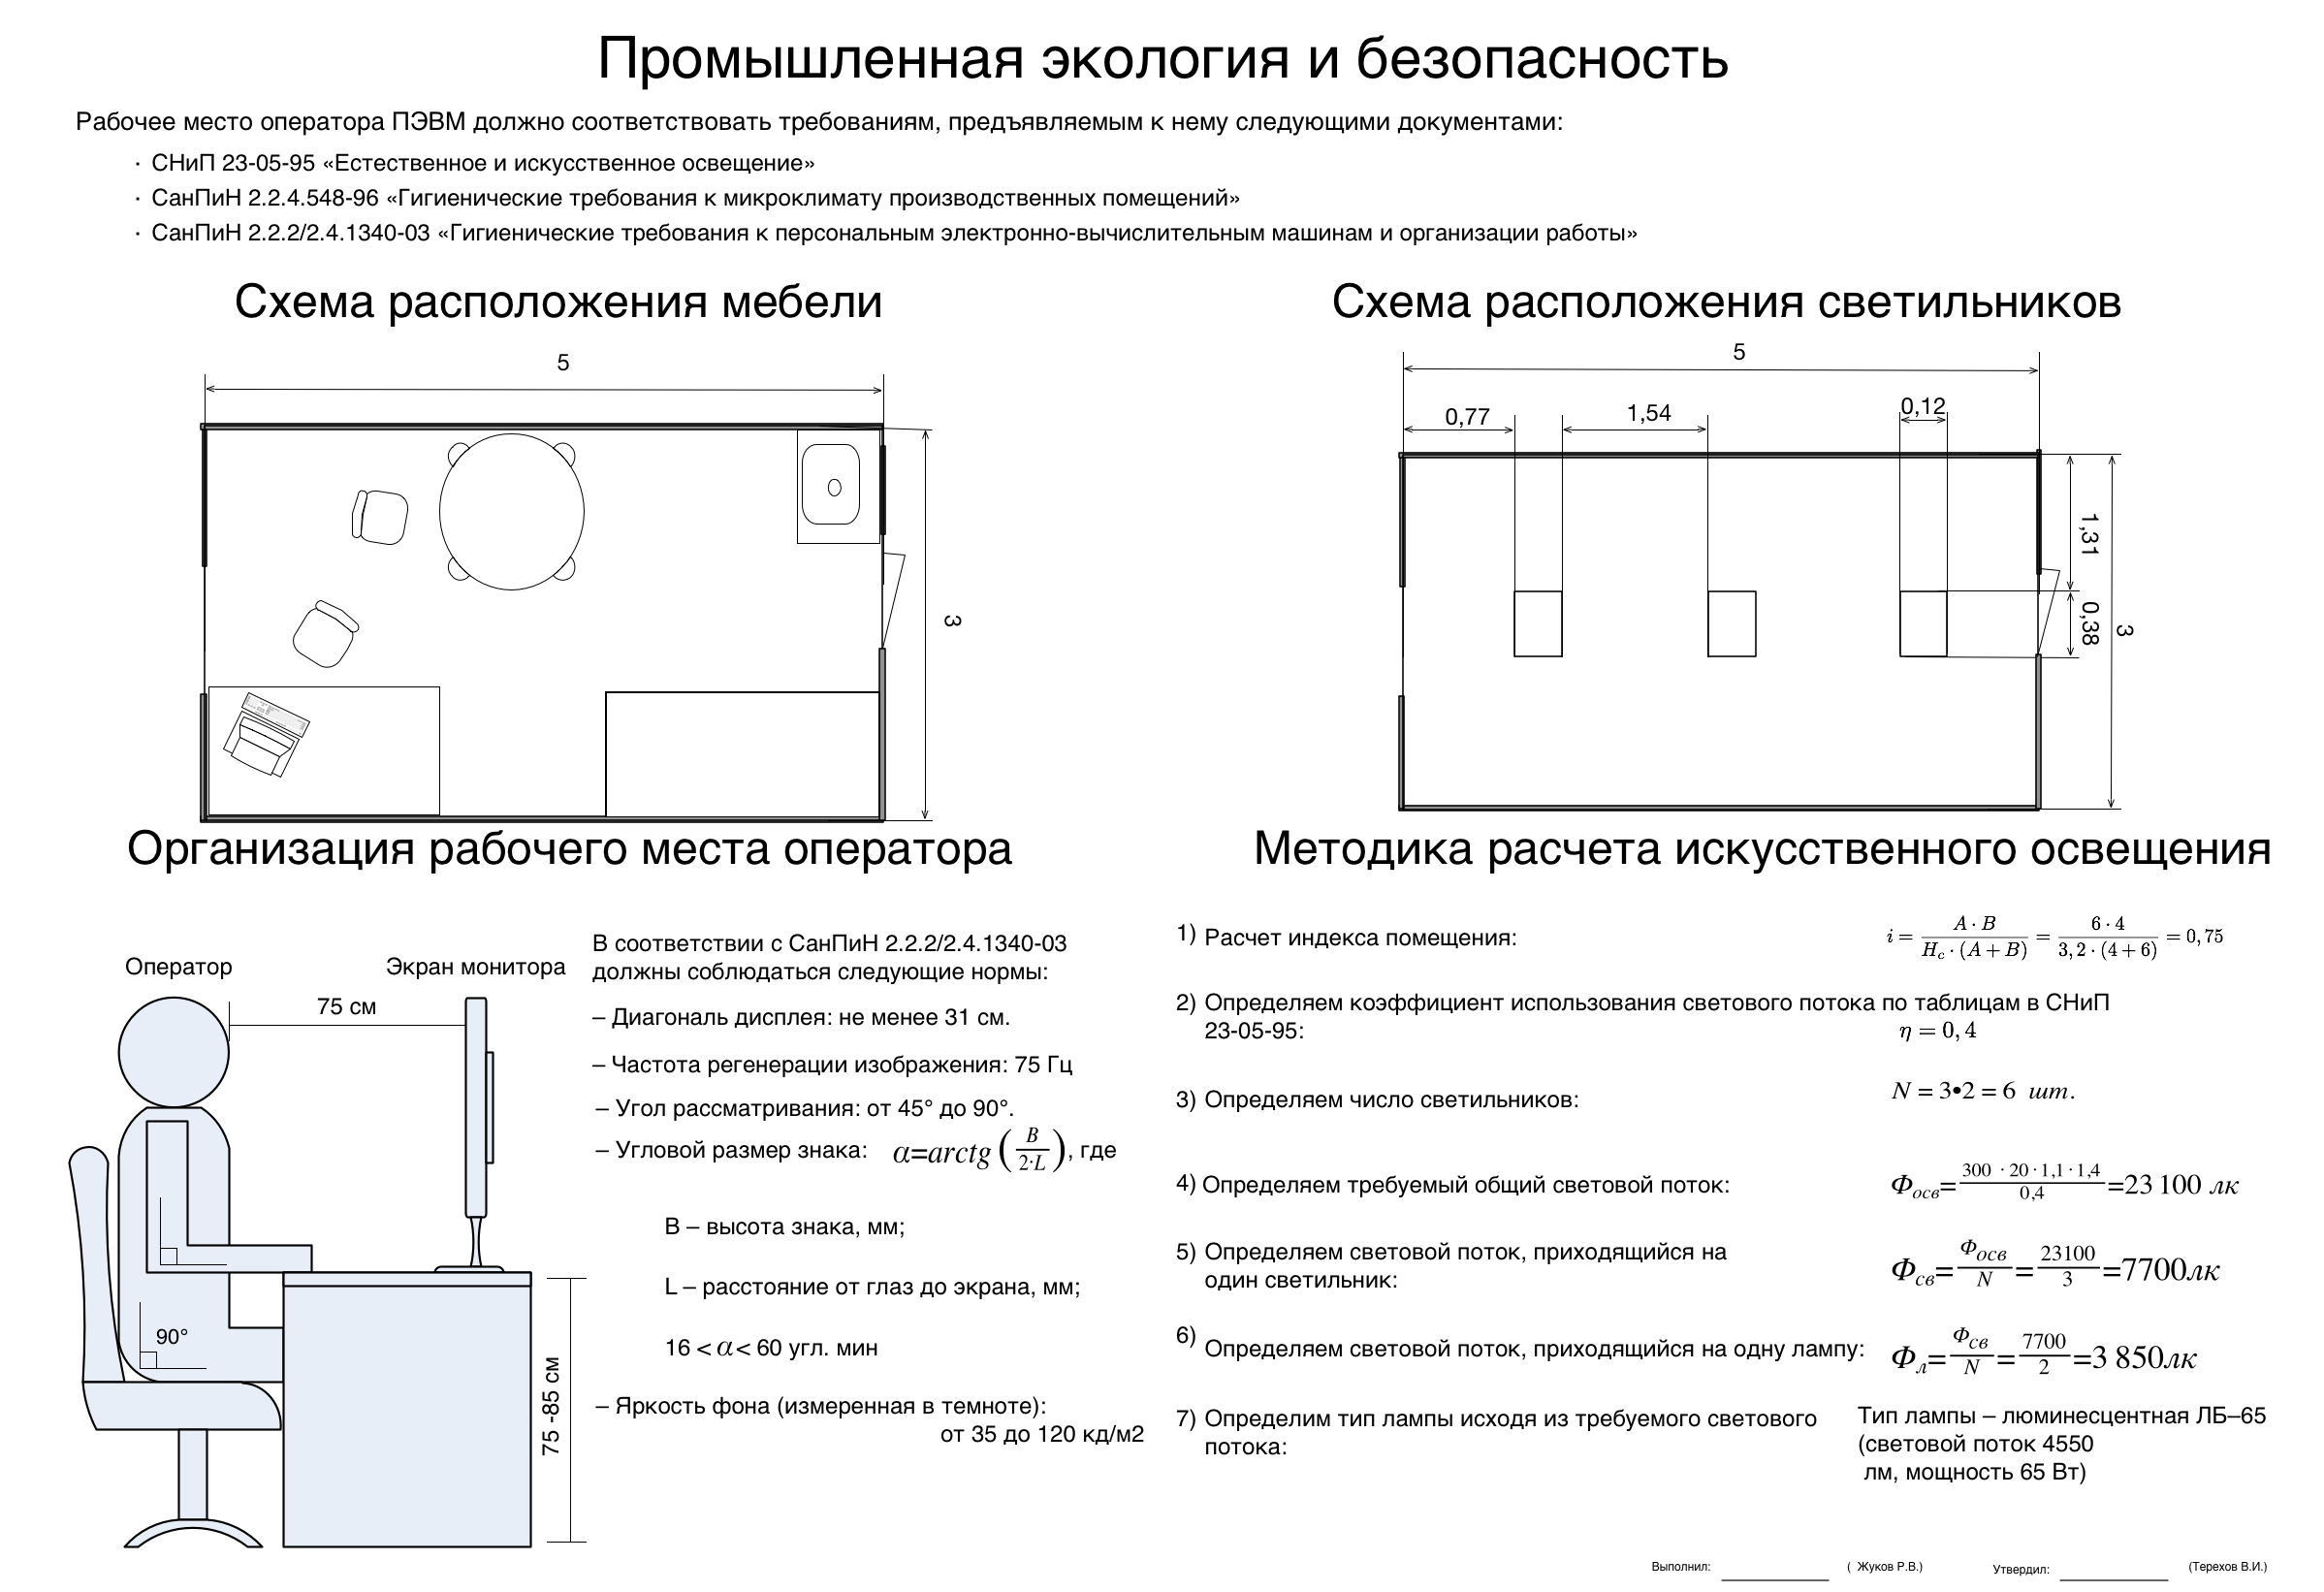
\includegraphics[width=0.99\linewidth]{pics/G10.png}}
\end{figure}
\end{landscape}
\clearpage
}
\end{document}